\documentclass{article}

% -----------------
% Packages
% -----------------
\usepackage{nomencl}
\usepackage[
  left=2cm,
  right=2cm,
  top=2.5cm,
  bottom=2cm
]{geometry}
\usepackage[bottom]{footmisc}
\usepackage{setspace}
\usepackage{graphicx}
\usepackage{subcaption}
\usepackage{float}
\usepackage{import}
\usepackage{tabularx}
\usepackage{comment}
\usepackage{fancyhdr}
\usepackage{tocloft}
\usepackage{wrapfig}
\usepackage{amsmath}
\usepackage{amssymb}
\usepackage{titlesec}
\usepackage{booktabs}
\usepackage[justification=centering]{caption}
\captionsetup{font=onehalfspacing}
\usepackage{listings}
\usepackage{xcolor}
\usepackage{ulem}
\usepackage{multirow}
\usepackage{url}
\usepackage{longtable, array, enumitem}
\usepackage[table]{xcolor}


\definecolor{codegray}{rgb}{0.95,0.95,0.95}
\definecolor{keywordcolor}{rgb}{0.36,0.54,0.66}
\definecolor{commentcolor}{rgb}{0,0.5,0}

\lstset{
    backgroundcolor=\color{codegray},
    basicstyle=\ttfamily\footnotesize,
    keywordstyle=\color{keywordcolor}\bfseries,
    commentstyle=\color{commentcolor}\itshape,
    stringstyle=\color{red},
    numbers=left,
    numberstyle=\tiny\color{gray},
    stepnumber=1,
    numbersep=5pt,
    showspaces=false,
    showstringspaces=false,
    showtabs=false,
    frame=single,
    tabsize=4,
    captionpos=b,
    breaklines=true,
    breakatwhitespace=false,
    escapeinside={(*@}{@*)}
}

% -----------------
% Section spacing
% -----------------
\titlespacing*{\subsection}
  {0pt}
  {2ex plus 1ex minus .2ex}
  {0em}

\titlespacing*{\subsubsection}
  {0pt}
  {2ex plus 1ex minus .2ex}
  {0em}

% --------------------------------------------
% Allow deeper sectioning (up to level 5)
% --------------------------------------------
\setcounter{secnumdepth}{5}
\setcounter{tocdepth}{3}

% --- Define counters for deeper levels ---
\makeatletter

\newcounter{subsubsubsection}[subsubsection]
\renewcommand{\thesubsubsubsection}{\thesubsubsection.\arabic{subsubsubsection}}

\newcounter{subsubsubsubsection}[subsubsubsection]
\renewcommand{\thesubsubsubsubsection}{\thesubsubsubsection.\arabic{subsubsubsubsection}}

% --- Define ToC formatting for new levels ---
\newcommand{\l@subsubsubsection}{\@dottedtocline{4}{7em}{3em}}
\newcommand{\l@subsubsubsubsection}{\@dottedtocline{5}{10em}{4em}}

\makeatother

% --- Define visual formatting for deep levels ---
\newcommand{\subsubsubsection}[1]{%
  \refstepcounter{subsubsubsection}%
  \par\vspace{0.5\baselineskip}%
  \noindent\textbf{\thesubsubsubsection\ #1}\par\vspace{0.25\baselineskip}%
  \addcontentsline{toc}{subsubsubsection}{\protect\numberline{\thesubsubsubsection}#1}%
}

\newcommand{\subsubsubsubsection}[1]{%
  \refstepcounter{subsubsubsubsection}%
  \par\vspace{0.25\baselineskip}%
  \noindent\textbf{\thesubsubsubsubsection\ #1}\par\vspace{0.25\baselineskip}%
  \addcontentsline{toc}{subsubsubsubsection}{\protect\numberline{\thesubsubsubsubsection}#1}%
}

% -----------------
% Paragraph spacing
% -----------------
\setlength{\parindent}{0pt}
\setlength{\parskip}{1em}

% -----------------
% Nomenclature setup
% -----------------
\usepackage{nomencl}
\makenomenclature
\setlength{\nomlabelwidth}{4.7cm}
% \renewcommand{\nompreamble}{(The nomenclature must respect the following order: latin symbols, Greek symbols, acronyms. Within each category of symbols, follow alphabetic order. An example is provided below)}

% -----------------
% Line spacing
% -----------------
\onehalfspacing

% -----------------
% Header/footer setup
% -----------------
\pagestyle{fancy}
\fancyhf{}
\fancyhead[L]{Thesis C}
\fancyhead[R]{Nathan Sivalingam}
\fancyfoot[C]{\thepage}
\renewcommand{\headrulewidth}{0pt}
\renewcommand{\footrulewidth}{0pt}
\setlength{\headheight}{15pt}
\setlength{\headsep}{25pt}

% Unnumbered subsection that still appears in the ToC
\newcommand{\subsectiontoc}[1]{%
  \subsection*{#1}%
  \addcontentsline{toc}{subsection}{#1}%
}

% -----------------
% Document start
% -----------------
\begin{document}

% -----------------
% Title Page
% -----------------
\begin{center}
    
        \begin{figure}[H] % [H] positions the figure "here". For more information of positioning of Figure see: https://www.overleaf.com/learn/latex/Positioning_of_Figures and inserting an image here: https://www.overleaf.com/learn/latex/Inserting_Images
            \centering %Centres the figure in the middle of the page
            \includegraphics[width=7cm]{Figures/UNSW Logo.jpg} % inserts the figure from the Figures folder (note figures need to be uploaded before inserting).
        \end{figure}
        
        \LARGE
        School of Mechanical and Manufacturing Engineering \\
        
        Faculty of Engineering \\

        UNSW Sydney

        \vspace{1cm}
        
        \LARGE
        BY \\
        \vspace{0.5cm}
        
        \huge
        \textbf{Nathan Sivalingam} \\
        \vspace{0.5cm}
        
        \LARGE
        \textbf{An Investigation into the Height Effects of Vortex Generators on Photovoltaic Module Temperature Reduction under Forced Convection Conditions}
        \vspace{1cm}
        
        \LARGE
        Thesis submitted as a requirement for the degree of Bachelor of Engineering in Mechanical Engineering

        \vfill

        \large
        \begin{tabularx}{1\textwidth}{ 
  | >{\raggedright\arraybackslash}X 
  | >{\raggedright\arraybackslash}X 
  | } 
        \hline
        Submitted: 21 November 2025 & Student zID: z5359644 \\ 
        \hline
        Supervisor: Dr Charitha de Silva (UNSW) & PhD Candidate: Matthew Deng (UNSW)\\ 
        \hline
        \end{tabularx}

\end{center}


\thispagestyle{empty}
\pagebreak

% -----------------
% Front Matter
% -----------------
\pagenumbering{roman}

\input{Sections/Originality Statement}
\pagebreak
\section*{Abstract}

\addcontentsline{toc}{section}{Abstract}

\begin{comment}
Write a short abstract restating the main objectives of the project, your main findings and their significance. Do not exceed 100 words in the abstract. \\

The maximum length of the entire report is 50 pages, excluding appendices, bibliography and cover sheet / abstract / acknowledgements / nomenclature / table of contents / lists of figures and tables. Please note that, differently from the overall 50 page limit, the limits provided for each section (given later) are indicative. You can use Microsoft Word or other document editors such as LaTeX, InDesign, or OpenOffice, however font sizes and margins need to be very similar to this template. Please also refer to the course outline for details on the expectations regarding this document (marking criteria and rubrics).
\end{comment}

Photovoltaic modules play a central role in meeting the growing global demand for renewable energy, yet their electrical efficiency declines as operating temperature rises. Vortex generators have been proposed as a means of enhancing convective heat transfer and mitigating this thermally induced performance loss; however, the height-dependent effects of vortex generators on photovoltaic module temperature reduction remain insufficiently understood. To address this gap, forced-convection wind-tunnel experiments were conducted using cylindrical vortex generators of three heights (15~mm, 75~mm, and 150~mm), with module temperatures measured across multiple airflow velocities and analysed through MATLAB-based post-processing, energy-balance correlations, and supporting CFD analysis. It was found that centrally positioning the thermal camera artificially increased cooling due to tripod-generated Kármán vortices, and that relocating the camera to the side removed this interference and produced reliable, unaffected measurements. Ambient temperature was also found to fundamentally alter vortex-generator behaviour: the 15~mm array exhibited a reduced module-temperature-to-ambient-temperature gradient compared with the baseline (0.9 versus 1.2--1.3), leading to heating at lower ambient temperatures and a transition to cooling at higher temperatures as bottom-surface convection increased. Across all wind speeds, the 15~mm array was the most effective configuration, producing the least heating at low ambient temperatures (e.g., 1.12~\textdegree C at 1~m/s) and achieving up to 0.99~\textdegree C of cooling at higher ambient temperatures, with cooling initiating at a lower threshold than the other tested heights. Overall, the results show that vortex-generator height governs cooling performance through its influence on bottom-surface convection, revealing a clear link between inlet flow area and module temperature.


\pagebreak
\section*{Acknowledgments}

\addcontentsline{toc}{section}{Acknowledgments}

I would like to express my deepest gratitude to Dr Charitha de Silva for your exceptional guidance, support, and mentorship throughout this thesis. Your willingness to offer help beyond expectation, whether through detailed feedback, thoughtful direction, or encouragement during challenging stages, has been invaluable to both my academic development and the success of this project. I am sincerely thankful for the trust you placed in me and for the opportunity to grow under your supervision.

I extend my sincere appreciation to Matthew Deng, whose dedication to this project has been truly inspiring. Thank you for running experimental tests on weekends, for troubleshooting ideas through long discussions, and for consistently sharing your knowledge with patience and enthusiasm. Your support has been invaluable, and it has been a privilege to learn from you and work alongside you. As you continue this project beyond the completion of my thesis, I wish you every success in both your PhD and your future career.

I would also like to thank Shubhneet Sodhi, without whom this journey would not have been the same. From late-night calls to early-morning problem-solving sessions, your support, friendship, and shared determination transformed an intimidating task into one of the most rewarding experiences of my time at university. I feel incredibly fortunate that we completed this thesis together. In the first trimester, I wrote that by the end we might finally feel as though we had earned the break. Now that the break is approaching, it is clear that the exhaustion we once felt has become a testament to that effort. This experience has reminded me that challenge is inseparable from purpose, and I remain grateful for such exceptional company.

Finally, I am grateful to my family and friends for their unwavering patience and support. Your willingness to listen, even when I spoke at length about concepts far removed from your own interests, has meant more to me than I can express. Your kindness, encouragement, and constant presence have made me feel incredibly fortunate. Any success I achieve, I owe to all of you.

\pagebreak

% Reduce ToC spacing
\setlength{\cftbeforesecskip}{2pt}
\setlength{\cftbeforesubsecskip}{1pt}

% Table of Contents
\tableofcontents
\pagebreak

\cleardoublepage
\addcontentsline{toc}{section}{List of Figures}
\listoffigures
\pagebreak

\cleardoublepage
\addcontentsline{toc}{section}{List of Tables}
\listoftables
\pagebreak

\addcontentsline{toc}{section}{Nomenclature}

% The nomenclature section is created here (variables and definitions can be edited below).
\nomenclature[3KE]{K.E.}{Kinetic energy of the emitted electron [J]}
\nomenclature[1hp]{\(h_p\)}{Planck's constant [$6.6261\times 10^{-34}$ Js]}
\nomenclature[1f0]{\(f_0\)}{Threshold frequency [Hz]}
\nomenclature[2phi]{\(\phi_0\)}{Work function [J]}
\nomenclature[2eta]{\(\eta\)}{Electrical efficiency [-]}
\nomenclature[1VOC]{\(V_{\text{OC}}\)}{Open circuit voltage [V]}
\nomenclature[1ISC]{\(I_\text{SC}\)}{Short circuit current [A]}
\nomenclature[3FF]{FF}{Fill factor [-]}
\nomenclature[1Pin]{\(P_\text{in}\)}{Input power [W]}
\nomenclature[1P]{\(P\)}{Perimeter [m]}
\nomenclature[1J0I0]{\(J_0,I_0\)}{Dioide saturation current [A/$\mathrm{m^2}$]}
\nomenclature[1q]{\(q\)}{Elementary charge [$\mathrm{1.602 \times 10^{-19}\ C}$]}
\nomenclature[1kb]{\(k_b\)}{Boltzmann's constant [$\mathrm{1.381 \times 10^{-23}\ J/K}$]}
\nomenclature[2sigma]{\(\sigma\)}{Stefan-Boltzmann constant [$\mathrm{5.670 \times 10^{-8}\ W/m^2K^4}$]}
\nomenclature[1T]{\(T\)}{Temperature [K]}
\nomenclature[1Eg]{\(E_g\)}{Band gap energy [eV]}
\nomenclature[2zeta]{\(\zeta\)}{Ideality factor [-]}
\nomenclature[1IL]{\(I_L\)}{Light generated current [$\mathrm{A/m^2}$]}
\nomenclature[1JSC]{\(J_\text{SC}\)}{Short circuit current density [$\mathrm{A/m^2}$]}
\nomenclature[1A]{\(A,A_c\)}{Cross-sectional area [$\mathrm{m^2}$]}
\nomenclature[1voc]{\(v_\text{OC}\)}{Normalised open circuit voltage [-]}
\nomenclature[1Qcond]{\(\dot{Q}_\mathrm{cond}\)}{Rate of conductive heat transfer [W]}
\nomenclature[1Qcondvg]{\(\dot{Q}_\mathrm{cond,vg}\)}{Rate of conductive heat transfer from the photovoltaic module to a single vortex generator [W]}
\nomenclature[1Qcondarray]{\(\dot{Q}_\mathrm{cond,array}\)}{Rate of conductive heat transfer from the photovoltaic module to the vortex generator array [W]}
\nomenclature[1Qconv]{\(\dot{Q}_\mathrm{conv}\)}{Rate of convective heat transfer [W]}
\nomenclature[1Qconvtop]{\(\dot{Q}_\mathrm{conv,top}\)}{Rate of convective heat transfer from the top surface of the photovoltaic module [W]}
\nomenclature[1Qconvbottom]{\(\dot{Q}_\mathrm{conv,bottom}\)}{Rate of convective heat transfer from the bottom surface of the photovoltaic module [W]}
\nomenclature[1k]{\(k\)}{Thermal conductivity [$\mathrm{W/mK}$]}
\nomenclature[1kair]{\(k_\mathrm{air}\)}{Thermal conductivity of air [$0.0259\ \mathrm{W/mK}$]}
\nomenclature[1kpla]{\(k_\mathrm{PLA}\)}{Thermal conductivity [$\mathrm{W/mK}$]}
\nomenclature[2DeltaT]{\(\Delta T\)}{Temperature difference [K]}
\nomenclature[2Deltax]{\(\Delta x\)}{Material thickness [m]}
\nomenclature[1As]{\(A_s\)}{Surface area [$\mathrm{m^2}$]}
\nomenclature[1Qrad]{\(\dot{Q}_\mathrm{rad}\)}{Rate of radiative heat transfer [W]}
\nomenclature[1Qradtop]{\(\dot{Q}_\mathrm{rad,top}\)}{Rate of conductive heat transfer from the top surface of the photovoltaic module [W]}
\nomenclature[1Qradbottom]{\(\dot{Q}_\mathrm{rad,bottom}\)}{Rate of conductive heat transfer from the bottom surface of the photovoltaic module [W]}
\nomenclature[1Qloss]{\(\dot{Q}_\mathrm{loss}\)}{Total heat transfer from the photovoltaic module to the environment [W]}
\nomenclature[2varepsilon]{\(\varepsilon\)}{Surface emissivity [-]}
\nomenclature[2varepsilonradbottom]{\(\varepsilon_\mathrm{rad,bottom}\)}{Surface emissivity for the bottom surface of the photovoltaic module [-]}
\nomenclature[2varepsilonradtop]{\(\varepsilon_\mathrm{rad,top}\)}{Surface emissivity for the top surface of the photovoltaic module [-]}
\nomenclature[1Ts]{\(T_s\)}{Surface temperature [K]}
\nomenclature[1Tsurr]{\(T_\mathrm{surr}\)}{Temperature of the surrounding environment [K]}
\nomenclature[1h]{\(h, h_\mathrm{conv}\)}{Convective heat transfer coefficient [$\mathrm{Wm^{-2} K^{-1}}$]}
\nomenclature[1hcyl]{\(h_\mathrm{cyl}\)}{Convective heat transfer coefficient for a cylindrical vortex generator in cross flow [$\mathrm{Wm^{-2} K^{-1}}$]}
\nomenclature[1hconvbottom]{\(h_\mathrm{conv,bottom}\)}{Convective heat transfer coefficient for the bottom surface of the photovoltaic module [$\mathrm{Wm^{-2} K^{-1}}$]}
\nomenclature[1hconvtop]{\(h_\mathrm{conv,top}\)}{Convective heat transfer coefficient for the top surface of the photovoltaic module [$\mathrm{Wm^{-2}K^{-1}}$]}
\nomenclature[1Tinf]{\(T_\infty\)}{Temperature of the surrounding fluid [K]}
\nomenclature[1g]{\(g\)}{Gravitational constant [$\mathrm{9.81\ m/s^2}$]}
\nomenclature[1F]{\(F\)}{Buoyant force [N]}
\nomenclature[1Fx]{\(F_x\)}{Component of the buoyant force parallel to the surface [N]}
\nomenclature[1Fy]{\(F_y\)}{Component of the buoyant force perpendicular to the plate [N]}
\nomenclature[2theta]{\(\theta\)}{Angle of inclination [$\mathrm{^\circ}$]}
\nomenclature[2thetab]{\(\theta_b\)}{Excess temperature at the fin base relative to the ambient air [K]}
\nomenclature[1RaL]{\(\mathrm{Ra_L}\)}{Rayleigh number [-]}
\nomenclature[2beta]{\(\beta\)}{Volumetric thermal expansion coefficient [1/K]}
\nomenclature[1Lc]{\(L_c\)}{Characteristic length [m]}
\nomenclature[1mdot]{\(\dot{m}\)}{Mass flow rate [kg/s]}
\nomenclature[1mfin]{\(m_\mathrm{fin}\)}{Fin parameter [-]}
\nomenclature[1Mfin]{\(M_\mathrm{fin}\)}{Fin conduction parameter [-]}
\nomenclature[2nu]{\(\nu\)}{Kinematic viscosity [$\mathrm{m^2/s}$]}
\nomenclature[2alpha]{\(\alpha\)}{Thermal diffusivity [$\mathrm{m^2/s}$]}
\nomenclature[1Ratheta]{\(\mathrm{Ra_\theta}\)}{Rayleigh number on an inclined plate [-]}
\nomenclature[1Nu]{\(\mathrm{Nu}\)}{Nusselt number [-]}
\nomenclature[1Nuforced]{\(\mathrm{Nu_\mathrm{forced}}\)}{Forced-convection Nusselt number [-]}
\nomenclature[1Nufree]{\(\mathrm{Nu_\mathrm{free}}\)}{Natural-convection Nusselt number [-]}
\nomenclature[1Numix]{\(\mathrm{Nu_\mathrm{mix}}\)}{Mixed-convection Nusselt number [-]}
\nomenclature[1C]{\(C\)}{Geometry and flow condition dependent constant [-]}
\nomenclature[1gamma]{\(\mathrm{\gamma}\)}{Rayleigh number exponent [-]}
\nomenclature[1m]{\(\mathrm{m}\)}{Reynolds number exponent [-]}
\nomenclature[1n]{\(\mathrm{n}\)}{Prandtl number exponent [-]}
\nomenclature[1u]{\(u\)}{Distance-specific fluid velocity [m/s]}
\nomenclature[2delta]{\(\delta\)}{Velocity boundary layer thickness [m]}
\nomenclature[2deltat]{\(\delta_t\)}{Thermal boundary layer thickness [m]}
\nomenclature[1ReD]{\(\mathrm{Re_D}\)}{Cylinder-specific Reynolds number [-]}
\nomenclature[2rho]{\(\rho\)}{Fluid density [$\mathrm{kg/m^3}$]}
\nomenclature[1V]{\(V\)}{Fluid velocity [m/s]}
\nomenclature[1D]{\(D\)}{Characteristic diameter [m]}
\nomenclature[2mu]{\(\mu\)}{Dynamic Viscosity [kg/ms]}
\nomenclature[1Nucyl]{\(\mathrm{Nu_{cyl}}\)}{Average nusselt number for cross flow over a cylinder [-]}
\nomenclature[1Re]{\(\mathrm{Re}, \mathrm{Re_L}\)}{Reynolds number [-]}
\nomenclature[1Gr]{\(\mathrm{Gr_L}\)}{Grashof number [-]}
\nomenclature[1Pr]{\(\mathrm{Pr}\)}{Prandtl number [-]}
\nomenclature[2deltax]{\(\delta_x\)}{Vortex generator spacing in the span-wise direction [mm]}
\nomenclature[2deltay]{\(\delta_y\)}{Vortex generator spacing in the stream-wise direction (m)}
\nomenclature[1Eblambda]{\(E_\mathrm{b \lambda}\)}{Spectral radiance of a blackbody [$\mathrm{W/m^3}$]}
\nomenclature[1Eindot]{\(\dot{E}_\mathrm{in}\)}{Rate of energy entering the control volume [J]}
\nomenclature[1Eoutdot]{\(\dot{E}_\mathrm{out}\)}{Rate of energy leaving the control volume [J]}
\nomenclature[1Egendot]{\(\dot{E}_\mathrm{gen}\)}{Rate of energy generation within the control volume [J]}
\nomenclature[1t]{\(t\)}{Time [s]}
\nomenclature[1Qindot]{\(\dot{Q}_\mathrm{in}\)}{Rate of heat entering the control volume [W]}
\nomenclature[1Qoutdot]{\(\dot{Q}_\mathrm{out}\)}{Rate of heat leaving the control volume [W]}
\nomenclature[1U]{\(U\)}{Internal energy [J]}
\nomenclature[1m]{\(m\)}{System mass [kg]}
\nomenclature[1N]{\(N\)}{Number of vortex generators in the vortex generator array [-]}
\nomenclature[1cp]{\(c_p\)}{Specific heat capacity at constant pressure [$\mathrm{J kg^{-1} K^{-1}}$]}
\nomenclature[2lambda]{\(\lambda\)}{Wavelength [$\mathrm{\mu m}$]}
\nomenclature[1Tb]{\(T_b\)}{Absolute temperature of a blackbody [K]}
\nomenclature[1Tf]{\(T_f\)}{Film temperature [K]}
\nomenclature[1C1]{\(C_1\)}{First radiation constant [$\mathrm{W\mu m^4/m^2}$]}
\nomenclature[1C2]{\(C_2\)}{Second radiation constant [$\mathrm{\mu mK}$]}
\nomenclature[3MTFHS]{MTFHS}{Multidirectional Tapered Fin Heat Sinks}
\nomenclature[3PCM]{PCM}{Phase Change Material}
\nomenclature[3NOCT]{NOCT}{Nominal Operating Cell Temperature}
\nomenclature[3PIV]{PIV}{Particle Image Velocimetry}
\nomenclature[3LWT]{LWT}{Large Wind Tunnel}
\nomenclature[3CFD]{CFD}{Computational Fluid Dynamics}
\nomenclature[3PLA]{PLA}{Polylactic Acid}
\nomenclature[3PDMS]{PDMS}{Polydimethylsiloxane}
\nomenclature[3DC]{DC}{Direct Current}
\nomenclature[3IR]{IR}{Infrared Radiation}
\nomenclature[3CSV]{CSV}{Comma-separated Values}
\nomenclature[3PV]{PV}{Photovoltaic Module}
\nomenclature[3RTD]{RTD}{Resistance-To-Digital converter}
\nomenclature[3VG]{VG}{Vortex Generator}
\nomenclature[3HSE]{HSE}{Health, Safety, and Environment}
\nomenclature[3AM]{AM}{Air Mass}
\nomenclature[1AL]{\(A_\mathrm{L}, A_\mathrm{lat}\)}{Lateral area exposed to air flow [$\mathrm{m^2}$]}
\nomenclature[1Atip]{\(A_\mathrm{tip}\)}{Circular cross-sectional area of cylindrical vortex generator [$\mathrm{m^2}$]}
\nomenclature[1d]{\(d\)}{Vortex generator diameter [m]}
\nomenclature[1r]{\(r\)}{Vortex generator radius [m]}
\nomenclature[1dx]{\(d_x\)}{Span-wise direction [m]}
\nomenclature[1dy]{\(d_y\)}{Stream-wise direction [m]}
\nomenclature[1M]{\(M\)}{Mach number [-]}
\nomenclature[1hstar]{\(h^*\)}{Ratio of the vortex generator height to the incoming boundary layer thickness [-]}
\nomenclature[1HVG]{\(H_\mathrm{VG}, L\)}{Vortex generator height [m]}
\nomenclature[1Tmodvg]{\(T_\mathrm{mod, vg}\)}{Temperature of the photovoltaic module under the influence of a vortex generator array [$^\circ \mathrm{C}$]}
\nomenclature[1Tmodbaseline]{\(T_\mathrm{mod,baseline}, T_\mathrm{module,baseline}\)}{Temperature of the photovoltaic module without the influence of a vortex generator array [$^\circ \mathrm{C}$]}
\nomenclature[1Tmod]{\(T_\mathrm{mod}\)}{Photovoltaic Module Temperature [$^\circ \mathrm{C}$]}
\nomenclature[1Tbase]{\(T_\mathrm{base}\)}{Temperature at the base of the vortex generator [K]}
\nomenclature[1Tamb]{\(T_\mathrm{amb}, T_\mathrm{ambient}\)}{Ambient temperature of the surrounding environment [$^\circ \mathrm{C}$]}
\nomenclature[1Lwakelaminar]{\(L_\mathrm{wake,laminar}\)}{The length of the laminar wake caused by a single cylindrical vortex generator [m]}
\nomenclature[1Lwaketurbulent]{\(L_\mathrm{wake,turbulent}\)}{The length of the turbulent wake caused by a single cylindrical vortex generator [m]}


\printnomenclature
\pagebreak

% Save the last roman page number
\newcounter{romanpages}
\setcounter{romanpages}{\value{page}}

% -----------------
% Main Matter
% -----------------
\pagenumbering{arabic}

\section{Introduction}
\begin{comment}
This section should introduce your topic (to a reader who is an engineer, but may not be fully familiar with your topic – this is for the benefit of readers other than your supervisor, i.e. the moderator or incoming future students). Here you need to provide an overview of what the field is, what your project is, why your project is important, and very briefly how you have organized your work. It should set up the literature review – the reader now knows roughly what they are reading about and what they are looking for in the coming section(s). \\
    
The introduction might run to about \textbf{1 to 2 pages}, assuming a figure or two showing something highly useful for the reader, such as a picture of the problem (perhaps with annotation), and maybe some kind of flowchart showing the workflow.

\end{comment}

Throughout history, reliance on non-renewable energy sources has been central to the rapid advancement of society, ultimately culminating in the emergence of the modern world. Today, the global population, now exceeding eight billion, remains heavily dependent on these energy sources for survival and continued development. However, the accelerated pace of advancement, coupled with rapid population growth, has led to the exploitation of these finite resources, resulting in significant environmental damage and their depletion. Fossil fuels such as coal, oil, and natural gas are responsible for approximately 89\% of global greenhouse gas emissions, which are recognised as the primary contributors to climate change \cite{ClientEarth2025}. Furthermore, the combustion of fossil fuels accounts for roughly 70\% of global air pollution, a major factor in an estimated 7 million premature deaths annually worldwide \cite{WorldHealthOrganization2024}. Moreover, proven oil reserves are decreasing by 3-4\% each year, as the rate of global extraction surpasses the discovery of new reserves, raising significant concerns about future supply shortages \cite{ExxonMobil2025}.

To address this challenge, the large-scale development of renewable energy sources was initiated. Wind turbines harnessed wind energy, dams and rivers captured the power of flowing water, and photovoltaic (PV) modules converted solar energy into electricity. This marked a global shift in energy dependence, with populations transitioning from non-renewable to sustainable energy sources. As of 2024, renewable energy sources account for approximately 40.9\% of global electricity generation, with solar power serving as the primary driver of this growth \cite{iea2024}.\par

As reliance on renewable energy sources grew, further investigation into their performance limitations became essential. One key issue identified was the reduction in the electrical efficiency of photovoltaic modules at elevated temperatures. In their seminal 1961 paper, \textit{Detailed Balance Limit of Efficiency of p-n Junction Solar Cells}, William Shockley and Hans Queisser established the theoretical maximum efficiency of silicon-based solar cells at approximately 30\% under standard illumination conditions \cite{Shockley1961}. Moreover, the electrical efficiency of a typical photovoltaic module generally ranges from 6\% to 20\% \cite{Dubey2013}. In 2010, H.G. Teo observed the inverse relationship between the electrical efficiency of photovoltaic modules and their operating temperature, noting that higher temperatures result in further efficiency losses \cite{Teo2012}. Specifically, for every degree Celsius above the optimal temperature of 25 \textdegree C, the electrical efficiency decreases by 0.5\% \cite{MorganKingThePanels}.\par

Thus, this thesis will investigate the height effects of vortex generators (VG) on photovoltaic module temperature reduction, with the aim of determining the optimal height to maximise cooling performance. To fulfil this aim, geometric parameters of the vortex generator array were selected for investigation, including the heights and shape of the vortex generators, as well as the position and spacing of the array. An experimental testing procedure, comprising an experimental method and a post-processing approach built on the work of previous thesis students, was then established. Past results from these earlier thesis campaigns were collected and used to validate the experimental procedure, ensuring confidence in its reliability. Following this validation, different vortex-generator heights were tested to identify the most effective height configuration.

Prior to establishing an experimental procedure, it is necessary to justify the focus on vortex generators and their height effects in reducing photovoltaic module temperatures. Accordingly, this thesis begins by examining existing methods designed to lower the operating temperature of photovoltaic modules. These methods are evaluated based on their effectiveness in reducing module temperature and, in turn, improving electrical efficiency. Through this review and assessment, vortex generators are identified as a promising cooling strategy, with the influence of their height emerging as an important gap in the literature warranting further investigation.

\pagebreak
\section{Literature Review}

\begin{comment}
This section can be developed starting from what you have reviewed and discussed in your previous reports, adjusted according to the feedback and indications provided by your supervisor(s). This section needs to flow logically, and this does not always imply that the material is chronological. By the end, the reader should have a clear appreciation of what the major work in the field was, why it is relevant to the current project, and where the unknowns and questions lie (research gaps) – these are the issues that you are going to address with your thesis research.

\subsection{\textbf{You can use subtitles like this to organize content within sections}}

An indicative length for the literature-review section is \textbf{~15 pages} (try to be concise and report significant information, rather than all information). Remember to reference properly any material that you obtain from literature or other sources. If you are unsure how to discuss literature properly, find a really good review paper on your topic, or if there isn’t one, a similar topic, and you will have a good example to refer to.
\end{comment}

\subsection{Principles of Photovoltaic Modules}
To understand the reduction in efficiency experienced by photovoltaic modules at increased temperatures, it is first necessary to examine the fundamental principles underlying their operation.\par

% Photovoltaic Module Definition + % Photoelectric Effect
Photovoltaic modules, commonly known as solar panels, are devices that convert sunlight into electrical energy \cite{EnelGreenPower2025PhotovoltaicModule, USDEPARTMENTofENERGY2024}. Sunlight is made up of massless particles called photons, which possess a certain amount of energy. When these photons strike the surface, they knock electrons off of it, known as photoelectrons. This is known as the photoelectric effect, shown in Figure \ref{fig:photoelectric_effect_diagram}.

\begin{wrapfigure}{r}{0.4\textwidth}
    \vspace{-2.5em}
    \centering
    \includegraphics[width=0.4\textwidth]{Figures/photoelectric_effect_diagram.png}
    \caption{Photoelectric Effect Diagram \cite{KhanAcademy2025PhotoelectricEffect}.}
    \label{fig:photoelectric_effect_diagram}
\end{wrapfigure}

The photoelectric effect will only occur if the frequency of the radiation is greater than the threshold frequency of the metal. The threshold frequency is the minimum frequency of light that causes electrons to be emitted from a material. The proportional relationship that exists between the threshold frequency, $f_0$, and the work function, $\phi_0$, is shown in Equation \ref{eq:work_function}.
\begin{equation}
    h_pf_0 = \phi_0+\text{K.E.}
    \label{eq:work_function}
\end{equation}
The work function refers to the minimum amount of energy needed to remove an electron from a metal surface. If photons with enough energy hit the surface, they can transfer their energy to the electrons allowing them to escape. If the energy of the incident photons is less than the work function, no electrons will be emitted, regardless of light intensity \cite{ScienceABC2023}.\par

% An Explanation of How Photovoltaic Modules Work
A photovoltaic module is made up of multiple photovoltaic cells, commonly known as solar cells. Each photovoltaic cell is made of semiconductor material, which is placed between the conductive layers. The most common semiconductor material used to make photovoltaic cells is silicon, accounting for 95\% of photovoltaic modules sold worldwide \cite{USDEPARTMENTofENERGY2024CellBasics}. These photovoltaic cells use the photovoltaic effect to convert solar energy into electrical energy.
\begin{figure}[H]
    \centering
    \vspace{-0.5em}
    \includegraphics[width=0.7\textwidth]
    {Figures/photovoltaic_cell_diagram.jpg}
    \vspace{-0.5em}
    \caption{Photovoltaic Cell Structure Diagram \cite{Gupta2020}.}
    \label{fig:photovoltaic_cell_diagram}
\end{figure}
\vspace{-1.5em}

As shown in Figure \ref{fig:photovoltaic_cell_diagram}, a silicon photovoltaic cell is composed of two different layers of silicon: an n-type silicon layer, which has additional electrons, and a p-type silicon layer, which has extra spaces for electrons, called holes.\par

Both the n-type and p-type silicon layers undergo a process known as doping; whereby specific impurities are intentionally introduced into an intrinsic semiconductor to enhance its electrical conductivity. The n- type silicon layer is doped with atoms such as arsenic or phosphorus, which possess one more valence electron than silicon atoms, thereby introducing additional free electrons into the material. Consequently, the n-type layer becomes negatively charged. Conversely, the p-type silicon layer is doped with elements such as boron or gallium, which possess one fewer valence electron than silicon atoms, creating electron deficiencies known as holes. As a result, the p-type layer acquires a positive charge. At the interface between the n-type and p-type layers, surplus electrons from the n-type region migrate to fill the holes in the p-type region, establishing an electric field across the p–n junction. This region is referred to as the depletion zone \cite{CircuitBread2019}.\par

When a photon strikes the silicon photovoltaic cell with the required energy, an electron is knocked out of its bond. Because of the electric field at the p-n junction, the negatively charged electron moves toward the n-side, while the resulting positively charged hole is attracted to the p-side. The free electrons are collected by thin metal fingers positioned at the top of the photovoltaic cell, before travelling through an external circuit. After electrical work is performed, the electrons are returned to the conductive aluminium sheet positioned at the back of the photovoltaic cell. Since electrons follow a continuous cycle and are the only moving components, there is no wear and tear, allowing photovoltaic cells to last for decades. \cite{TED-Ed2016} However, despite the absence of mechanical degradation, photovoltaic cells exhibit performance limitations under certain operating conditions.

\subsection{Performance Limitations of Photovoltaic Modules}
A major limitation of photovoltaic modules is their declining electrical efficiency, particularly at high temperatures. A review led by S. Dubey of Nanyang Technological University found that standard photovoltaic modules typically convert 6-20\% of incoming solar radiation into electrical energy. The remaining 80-94\% is mostly converted into heat, increasing the module’s temperature and further lowering its efficiency \cite{Dubey2013}.\par

% An active cooling system for photovoltaic modules - H.G. Teo
\begin{wrapfigure}{r}{0.65\textwidth}
    \vspace{-1.85em}
    \centering
    \includegraphics[width=0.65\textwidth]{Figures/electrical_efficiency_vs_temperature_pv_module.png}
    \vspace{-2em}
    \caption{Electrical efficiency as a function of PV temperature \cite{Teo2012}.}
    \label{fig:electrical_efficiency_vs_temperature_pv_module}
    \vspace{-2em} % <-- pulls text up closer
\end{wrapfigure}

A 2010 study led by H.G. Teo from the National University of Singapore refined Dubey et al.'s electrical efficiency range to 8-14\%. In the study, Teo et al. focused on comparing the electrical efficiency of photovoltaic modules under cooling and non-cooling conditions. Teo et al. observed that the electrical efficiency of the photovoltaic module decreased as the temperature of the module increased, as shown in Figure \ref{fig:electrical_efficiency_vs_temperature_pv_module}.

This inverse linear relationship between the temperature and the electrical efficiency of a photovoltaic module is attributed to the band gap reduction, which occurs as the module's temperature increases. % An explanation as to how increased module temperature leads to band gap reduction
In 1931, A.H. Wilson's paper, \textit{The Theory of Electronic Semi-Conductors}, introduced the idea that semiconductors have a small but finite band gap that affects their electrical conductivity \cite{Il1931}. The band gap represents the amount of energy that an electron must possess to jump from the valence band, where valence electrons are confined, to the conduction band. When valence electrons receive enough energy from an external source, they are able to undergo this band transition, which allows the material to conduct electricity \cite{CircuitBread2018}. As the temperature of the photovoltaic module increases, the valence electrons in the semiconductor material are excited. Thus, the energy required for an electron to transition from the valence band to the conduction band decreases, indicated by a reduced band gap \cite{RenewableTek2025}.\par

% Electrical efficiency of a photovoltaic module
\subsubsection{The Effect of Band Gap Reduction on Photovoltaic Module Performance}
To understand the proportional relationship between the band gap and the electrical efficiency, an inspection of the formula used to calculate the electrical efficiency of a photovoltaic cell, shown in Equation \ref{eq:pv_cell_efficiency_function}, is required \cite{HonsbergSolarEfficiency}.
\begin{equation}
    \eta = \frac{V_\text{OC}I_\text{SC}FF}{P_\text{in}}
    \label{eq:pv_cell_efficiency_function}
\end{equation}
The open circuit voltage, $V_\text{OC}$, short circuit current, $I_\text{SC}$, and fill factor, $FF$, are all affected by the band gap. Therefore, an investigation into the effect of a reduced band gap on these aforementioned variables is necessary to evaluate the impact that the band gap has on the electrical efficiency of the photovoltaic module.\par

% Open circuit voltage
\textbf{Open Circuit Voltage Analysis}\par
A 1994 study led by P. Baruch from the University of Paris derived a formula for determining the minimum value of the diode saturation current, as shown in Equation \ref{eq:minimum_diode_saturation_current}.
\begin{equation}
    J_0 = \frac{q}{k_b} \frac{15\sigma}{\pi^4} T^3 \int_{z}^{\infty} \frac{x^2}{e^x - 1}\,dx
    \label{eq:minimum_diode_saturation_current}
\end{equation}
where $z = \frac{E_G}{k_bT}$ \cite{Baruch1995}. A casual inspection of Equation \ref{eq:minimum_diode_saturation_current} reveals a relationship between the band gap energy, $E_g$, and the diode saturation current, $J_0$. However, it is not immediately obvious what the nature of the relationship is due to the complexity of the integral function.\par

\begin{figure}[h]
    \centering
    \begin{minipage}{0.495\textwidth}
        \centering
        \includegraphics[width=\textwidth]{Figures/diode_saturation_current_bandgap_graph.png}
        \caption{Diode saturation current as a function of band gap \cite{HonsbergOpen-CircuitVoltage}.}
        \label{fig:diode_saturation_current_bandgap_graph}
    \end{minipage}
    \hfill
    \begin{minipage}{0.465\textwidth}
        \vspace{-0.1em}
        \centering
        \includegraphics[width=\textwidth]{Figures/open-circuit_voltage_bandgap_graph.png}
        \caption{$V_\text{OC}$ as a function of band gap for a cell with AM 0 and AM 1.5 \cite{HonsbergOpen-CircuitVoltage}.}
        \label{fig:open-circuit_voltage_bandgap_graph}
    \end{minipage}
\end{figure}

Just over a decade later, Michael Y. Levy and Christiana Honsberg from the University of Delaware proposed a method to evaluate the integral in Baruch's formula \cite{Levy2006RapidApplications}. Then, in 2017, Honsberg worked with Stuart Bowden to graph the relationship between the diode saturation current and the band gap based on this method, as shown in Figure \ref{fig:diode_saturation_current_bandgap_graph}. Honsberg and Bowden used the diode saturation current values, $J_0$, from Figure \ref{fig:diode_saturation_current_bandgap_graph}, denoted as $I_0$ in Equation \ref{eq:open_circuit_voltage_function}, to calculate the open-circuit voltage, $V_\text{OC}$, as a function of the band gap. The linear proportional relationship between the band gap and the open-circuit voltage is shown in Figure \ref{fig:open-circuit_voltage_bandgap_graph}. Thus, the reduced band gap due to the increased temperature of the photovoltaic module leads to a decrease in the open-circuit voltage \cite{HonsbergOpen-CircuitVoltage}.
\begin{equation}
    V_{OC} = \frac{\zeta k_b T}{q} \times \ln\left(\frac{I_L}{I_0} + 1\right)
    \label{eq:open_circuit_voltage_function}
\end{equation}

% Short circuit current
\textbf{Short Circuit Current Analysis}\par
\begin{wrapfigure}{r}{0.5\textwidth}
    \vspace{-5.75em}
    \centering
    \includegraphics[width=\linewidth]{Figures/short_circuit_current_density_bandgap_graph.png}
    \caption{$J_\text{SC}$ as a function of band gap for a cell with AM 0 and AM 1.5. \cite{HonsbergShort-CircuitCurrent}}
    \label{fig:short_circuit_current_density_bandgap_graph}
\end{wrapfigure}

Honsberg and Bowden also graphed the relationship between the band gap and the short circuit current density, as shown in Figure \ref{fig:short_circuit_current_density_bandgap_graph}. From Figure \ref{fig:short_circuit_current_density_bandgap_graph}, it is evident that a band gap reduction corresponds to an increase in the short circuit current density. Equation \ref{short_circuit_current_function} shows a linearly proportional relationship between the short circuit current and the short circuit current density.
\begin{equation}
    I_\text{SC} = J_\text{SC}A
    \label{short_circuit_current_function}
\end{equation}
Therefore, a decrease in the band gap leads to an increase in the short-circuit current \cite{HonsbergShort-CircuitCurrent}.\par

% Fill Factor
\textbf{Fill Factor Analysis}\par
In 1981, M.A. Green of the University of New South Wales proposed an empirical expression for the fill factor, as shown in Equation \ref{eq:fill_factor_function}.
\begin{equation}
    FF = \frac{v_\text{OC} - \ln\ (v_\text{OC} + 0.72)}{v_\text{OC} + 1}
    \label{eq:fill_factor_function}
    \vspace{0.75em}
\end{equation}
where $v_\text{OC}$ is defined as a normalised $V_\text{OC}$: $v_\text{OC} = \frac{q}{nk_bT} V_\text{OC}$ \cite{Green1981}. As established earlier in Figure \ref{fig:open-circuit_voltage_bandgap_graph}, a band gap reduction corresponds to a decrease in the open-circuit voltage. An inspection of Equation \ref{eq:fill_factor_function} reveals that a decline in the open-circuit voltage and an increase in the temperature of the photovoltaic module causes a decrease in the fill factor. Therefore, it can be concluded that a band gap reduction causes a decrease in the fill factor.\par

% Resultant conclusion
To summarise, the band gap reduction that arises due to the increased temperature of the photovoltaic module causes a decrease in the open-circuit voltage, an increase in the short circuit current and a decrease in the fill factor. While the short circuit current does increase, it is ultimately outweighed by the decrease in the open-circuit voltage and fill factor, leading to a decrease in the module's electrical efficiency.

% Additional factors
\subsubsection{Environmental and Operational Factors Limiting Photovoltaic Module Performance}
In addition to temperature, other environmental factors like shade and air pollution limit the electrical efficiency of photovoltaic modules. A 2013 study led by A. Dolara from the Polytechnic University of Milan found that shade significantly affects the performance of photovoltaic modules. Dolara et al. observed a 31\% drop in the power generated by a single photovoltaic cell when 50\% of the cell was subjected to shade \cite{Dolara2013}. In 2001, E. Asl-Soleimani et al. from the University of Tehran concluded that air pollution also reduced the energy output of photovoltaic modules by up to 60\% \cite{Asl-Soleimani2001}. Furthermore, operational factors like poor module maintenance can lead to dust buildup, significantly reducing power generation. A review led by K. Hasan in 2021 stated a 60-70\% reduction in power generation due to the deposition of dust in humid conditions \cite{Hasan2022}. Although shade, air pollution, and dust accumulation influence photovoltaic module performance, this thesis focuses on temperature due to its unavoidable impact on module efficiency. In contrast to other environmental and operational factors that are site-specific or mitigable through maintenance, temperature rise is inherently linked to solar irradiation, the fundamental source of photovoltaic energy.

% Link the heat transfer paragraphs to the limitations paragraphs
In 1961, William Shockley and Hans Queisser published their paper, \textit{Detailed Balance Limit of Efficiency of p-n Junction Solar Cells}, in which they established the theoretical maximum efficiency of silicon-based solar cells to be approximately 30\% under standard illumination conditions \cite{Shockley1961}. In the real world however, photovoltaic cells are prevented from reaching this limit due to the factors previously discussed. Thus, due to the important role that photovoltaic modules play in the future of global energy, methods to reduce the impact that these factors have on the performance of photovoltaic modules are constantly being investigated.\par

In conjunction with establishing an inverse linear relationship between temperature and the electrical efficiency of photovoltaic modules, Teo et al. also observed that, under identical meteorological conditions, modules without active cooling operated at significantly higher temperatures than those with active cooling. Consequently, Teo et al.'s implementation of active cooling improved module efficiency from 8–9\% to 12–14\%, shown in Figure \ref{fig:electrical_efficiency_vs_temperature_pv_module} \cite{Teo2012}. As a result, to mitigate the reduction in electrical efficiency caused by increased photovoltaic module temperature, heat transfer-based cooling methods are investigated and employed worldwide.

\subsection{Heat Transfer in Photovoltaic Modules}
The fundamental concept of heat transfer is the process by which heat energy moves from one system or body to another as a result of a temperature difference. This transfer of heat can occur via conduction, convection or radiation. Figure \ref{fig:fundamental_concept_of_heat_transfer_diagram} demonstrates the fundamental concept of heat transfer in the context of a photovoltaic module.\par

\begin{figure}[H]
    \centering
    \includegraphics[width=1\textwidth]{Figures/fundamental_concept_of_heat_transfer_diagram.pdf}
    \vspace{-1.5em}
    \caption{Fundamental concept of heat transfer on a photovoltaic module. Adapted from \cite{HonsbergHeatModules}.}
    \label{fig:fundamental_concept_of_heat_transfer_diagram}
\end{figure}
\vspace{-1.5em}

In Figure \ref{fig:fundamental_concept_of_heat_transfer_diagram}, conductive heat transfer through the layers of the photovoltaic module and the mounting are observed. Additionally, heat is transferred from the surface of the photovoltaic module to the surrounding air via convection. Finally, the module emits thermal radiation to its surroundings, contributing to radiative heat transfer. In 2020, P. Dwivedi from the Maulana Azad National Institute of Technology, Bhopal, analysed the percentage distribution of heat loss across the different modes of heat transfer, shown in Table \ref{tab:heat_loss_from_pv_module} \cite{Dwivedi2020}.

\renewcommand{\arraystretch}{1.5} % increase vertical spacing
\begin{table}[h]
    \centering
    \caption{Heat loss from photovoltaic module \cite{Dwivedi2020}.}
    \begin{tabularx}{\textwidth}{l >{\hspace{4cm}}X l} % add horizontal space to middle column
        \toprule
        \textbf{S. No} & \textbf{Heat loss from module} & \textbf{Percentage (\%)} \\
        \midrule
        1 & Conduction through mounting & 2 \\
        2 & Convection from top surface & 42 \\
        3 & Convection from bottom surface & 24 \\
        4 & Radiation from top surface & 21 \\
        5 & Radiation from bottom surface & 11 \\
        \bottomrule
    \end{tabularx}
    \label{tab:heat_loss_from_pv_module}
\end{table}
\renewcommand{\arraystretch}{1} % reset back to default

An inspection of Table \ref{tab:heat_loss_from_pv_module} reveals that convection is the dominant mode of heat transfer in photovoltaic modules. Consequently, a given percentage increase in the rate of convective heat transfer will have a greater impact on overall module heat dissipation than an equivalent increase in conductive or radiative heat transfer. Therefore, the following subsections will examine the effectiveness of conduction-, convection-, and radiation-based cooling methods in reducing photovoltaic module temperatures to enhance overall efficiency, with particular emphasis on convection-based approaches.

\subsubsection{Conduction}
Conduction is the transfer of energy from the more energetic particles of a substance to the adjacent less energetic ones because of interactions between the particles. The formula commonly used to calculate the rate of heat conduction is shown in Equation 7 \cite{engel2014IntroductionAndBasicConcepts}.
\begin{equation}
    \dot{Q}_\text{cond}=-kA\frac{\Delta T}{\Delta x}
\end{equation}

Several conduction-based cooling methods have been widely adopted, with heat sinks and phase change materials (PCMs) being among the most prominent. A heat sink is a component used in thermal management strategies to transfer heat effectively. Its design is optimised to dissipate heat \cite{Kumar2024}. The use of a heat sink increases the cross-sectional area that the heat is being transferred to, denoted as $A$ in Equation 7. Through further inspection of Equation 7, it is observed that the increased cross-sectional area, $A$, results in an increased rate of conductive heat transfer, $\dot{Q}_\text{cond}$. A study led by S.N. Razali from the National University of Malaysia investigated the effect of
multidirectional tapered fin heat sinks (MTFHS) on photovoltaic modules. Razali et al. found that the proposed MTFHS reduced the module’s temperature by 12 \textdegree C, indicating enhanced conductive heat transfer, which consequently improved the photovoltaic module’s efficiency by 1.53\% \cite{Razali2023}.\par

A phase change material is a material that can change its state from solid to liquid and vice versa by releasing and storing thermal energy \cite{Nicholas2019}. When the surrounding temperature rises above the PCM’s melting point, it liquefies, drawing heat away from the photovoltaic module. Conversely, when the temperature drops below the melting point, the PCM solidifies, releasing the stored heat back into the environment. A 2023 study by B. Hussain and colleagues at the Capital University of Science \& Technology found that incorporating PCM lowered the surface temperature of photovoltaic modules by 13.1 \textdegree C, resulting in a 6.85\% increase in efficiency \cite{Hussain2023}.

\subsubsection{Radiation}
Radiation is the energy emitted by matter in the form of electromagnetic waves (or photons) due to changes in the electronic configurations of the atoms or molecules. In the context of heat transfer, the focus is on thermal radiation, which is the energy emitted by bodies due to their temperature. The formula 
commonly used to calculate the rate of radiative heat transfer is shown in Equation 8 \cite{engel2014IntroductionAndBasicConcepts}.
\begin{equation}
    \dot{Q}_\text{rad} = \varepsilon \sigma A_s (T_s^4-T_{surr}^4)
\end{equation}
In 2018, a study led by B. Zhao from the University of Science and Technology of China investigated the performance impact of radiation-based cooling methods on photovoltaic modules. Zhao et al. modified a photovoltaic module by adding a polydimethylsiloxane (PDMS) film on its top surface. PDMS is known to have high emissivity in the mid-infrared range (8-13) micrometres \cite{Song2020}. Through an inspection of Equation 8, it is observed that an increased emissivity, $\varepsilon$, causes an increase in the rate of radiative heat transfer, $\dot{Q}_\text{rad}$. In theory, the increased radiative heat transfer of the photovoltaic module lowers the module’s temperature and improves its efficiency. However, Zhao et al. found that the temperature of the photovoltaic module was only reduced by 1.75 K in the ideal case. Furthermore, this result was achieved using a simulated environment. Thus, Zhao’s team concluded that enhanced radiative cooling offers limited practical benefit for photovoltaic module temperature reduction \cite{Zhao2018}.

\subsubsection{Convection}
Convection is the mode of energy transfer between a solid surface and the adjacent liquid or gas that is in motion. The formula commonly used to calculate the rate of convective heat transfer can be expressed by Newton’s law of cooling, shown in Equation 9 \cite{engel2014IntroductionAndBasicConcepts}.
\begin{equation}
    \dot{Q}_\text{conv} = hA(T_s-T_\infty)
\end{equation}
Convection is not a fundamental heat transfer mechanism; rather, it is a combined phenomenon, where heat conduction occurs in the presence of fluid motion. Convection can be broadly categorised into two types: natural convection, also referred to as free convection, and forced convection \cite{engel2014FundamentalsOfConvection}.

\textbf{Natural Convection \& Relevant Cooling Methods}\par
\begin{wrapfigure}{r}{0.4\textwidth}
    \centering
    \vspace{-4.5em}
    \includegraphics[width=0.9\linewidth, trim=0 0 0 15, clip]{Figures/cooling_of_boiled_egg_natural_convection.pdf}
    \vspace{-1.5em}
    \caption{The cooling of a boiled egg from natural convection  
    \cite{engel2014IntroductionAndBasicConcepts}.}
    \label{fig:natural_convection_egg}
    \vspace{-2em}
\end{wrapfigure}

Natural convection is the process by which heat transferred to a fluid raises its temperature, reducing its density and generating buoyant forces. These forces cause the warmer, lighter fluid to rise, carrying the absorbed heat to 
another location where it can be dissipated \cite{Zohuri2020}. Figure \ref{fig:natural_convection_egg} illustrates natural convective heat transfer in the context of cooling a hot egg.

\textit{Tilt Angle Optimisation}\par
The tilt angle of a photovoltaic module significantly influences natural convective heat transfer, as it alters the buoyancy-driven airflow around the module’s surface. A 2021 study led by A. Abdulmunem from the University of Malaya, Malaysia, investigated the impact of tilt angle on the performance of photovoltaic systems. Abdulmunem et al. observed that as the tilt angle increased from 0\textdegree  (horizontal) to 90\textdegree (vertical), the temperature reduction in the photovoltaic cell increased from -0.4\% to -12\%. This trend was attributed to enhanced natural convective heat transfer which acts to improve photovoltaic module efficiency. Consequently, Abdulmunem et al. concluded that 
increasing the tilt angle of the photovoltaic module away from the horizontal axis and towards the vertical axis improves the rate of convective heat transfer \cite{Abdulmunem2021}.

\textit{Natural Convection Boundary Layers}\par
To understand the effect of the tilt angle on natural convective heat transfer, it is necessary to first understand the velocity and thermal boundary layers. The velocity boundary layer describes how the fluid’s motion adjusts from being stationary at the surface to moving freely away, while the thermal boundary layer describes how heat diffuses into or from the fluid at the surface. The thermal and velocity boundary layers are interconnected, with fluid motion influencing heat transfer, and their relative thickness depends on the fluid’s properties. The relationship between the thermal and velocity boundary layers is characterised by the Prandtl number, Pr.\par

As shown in Figure \ref{fig:horizontal_plate_nc}, at lower tilt angles (near horizontal), the heated air tends to remain attached to the surface for a longer duration, as the buoyancy forces are predominantly vertical. This results in the formation of a thicker and more stable thermal boundary layer, which promotes relatively weak convection. In contrast, as shown in Figure \ref{fig:inclined_plate_nc}, when the surface aligns more closely with the direction of the buoyant forces, the hot air can rise more freely along the surface. This facilitates a thinner thermal boundary layer and an increased air velocity near the surface, thereby enhancing convective heat transfer.

\begin{figure}[h]
    \centering
    \vspace{1em}
    \begin{minipage}{0.48\linewidth}
        \centering
        \includegraphics[width=0.66\linewidth]{Figures/horizontal_plate_nc.jpg}
        \caption{Natural convective heat transfer on a horizontal plate. Adapted from \cite{engel2014NaturalConvection}.}
        \label{fig:horizontal_plate_nc}
    \end{minipage}
    \hfill
    \begin{minipage}{0.48\linewidth}
        \centering
        \includegraphics[width=0.8\linewidth]{Figures/inclined_plate_nc.jpg}
        \caption{Natural convective heat transfer on a inclined plate. Adapted from \cite{engel2014NaturalConvection}.}
        \label{fig:inclined_plate_nc}
    \end{minipage}
\end{figure}

\textit{Tilt Angle Optimisation: A Theoretical Confirmation}\par
Abdulmunem’s conclusion is also in excellent agreement with the theoretical relationship between the photovoltaic module’s tilt angle and the natural convective heat transfer rate. The Rayleigh number, $\mathrm{Ra_L}$, which can be calculated using Equation 10, is the ratio of buoyancy forces and (the products of) thermal and momentum diffusivities \cite{engel2014NaturalConvection}.
\begin{equation}
    \mathrm{Ra_L} = \frac{g\beta(T_s-T_\infty)L_c^3}{\nu \alpha}
\end{equation}
For an inclined photovoltaic module between 0\textdegree and 60\textdegree, the gravitational force, $\mathrm{Ra_\theta}$, is replaced with $g\,sin(\theta)$, where $\theta$ represents the tilt angle between the horizontal axis and the photovoltaic module, shown in Figure 11.

\begin{wrapfigure}{r}{0.3\textwidth}  % 'r' = right, width = 40% of text width
    \vspace{-0.75em}
    \centering
    \includegraphics[width=\linewidth, trim=0 0 0 20, clip]{Figures/inclined_plate.pdf} 
    % trim=left bottom right top; top cropped by 50 units
    \vspace{-5.8em}
    \caption{Inclined photovoltaic module. Adapted from \cite{engel2014NaturalConvection}.}
    \label{fig:inclined_plate}
    \vspace{-1em}
\end{wrapfigure}

Thus, Equation 11 is the appropriate mathematical expression for the Rayleigh number of a tilted photovoltaic module, $\mathrm{Ra_\theta}$, \cite{engel2014NaturalConvection}.
\begin{equation}
    \mathrm{Ra_\theta} = \frac{g\, \sin(\theta)\, \beta\ (T_s-T_\infty)L_c^3}{\nu \alpha}
\end{equation}
A casual inspection of Equation 11 indicates that the Rayleigh number for a tilted photovoltaic module, $\mathrm{Ra_\theta}$, is directly proportional to the tilt angle, $\theta$, within the range of 0\textdegree to 60\textdegree\, \cite{engel2014NaturalConvection}. Therefore, increasing the tilt angle within this range results in a corresponding increase in the Rayleigh number.\par

The Nusselt number, Nu, is the ratio of convective to conductive heat transfer \cite{Basu2019}. For simple empirical correlations in natural convection, an exponential relationship exists between the average Nusselt number, Nu, and the relevant Rayleigh number, shown in Equation 12. \cite{engel2014NaturalConvection}
\begin{equation}
    \mathrm{Nu} = C\,\mathrm{Ra_\theta^\gamma}
\end{equation}
Therefore, the increase in the Rayleigh number leads to an increase in the Nusselt number. Moreover, Equation 13 reveals that an increase in the Nusselt number, Nu, causes an increase in the convective heat transfer coefficient, $h$, \cite{engel2014NaturalConvection}.
\begin{equation}
    h = \frac{\mathrm{Nu}\times k}{L_c}
\end{equation}
Finally, an inspection of Equation 9 reveals that an increase in the convective heat transfer coefficient, $h$, results in a higher convective heat transfer rate, $\dot{Q}_\mathrm{conv}$, thereby supporting Abdulmunem et al.’s experimental findings \cite{engel2014IntroductionAndBasicConcepts}.\par

While a vertical photovoltaic module improves natural convective heat transfer, it limits the surface area that is directly exposed to the sun, reducing power output. Thus, a tilt angle of 45\textdegree$\ $from the horizontal axis (as in earlier NOCT testing \cite{InternationalElectrotechnicalCommission2005}) is generally used in photovoltaic module testing because it represents more realistic conditions.

\textit{Comparing Natural and Forced Convection Effects in Photovoltaic Module Temperature Reduction}\par
Natural convection-based cooling methods can effectively reduce an object’s temperature; however, in photovoltaic modules, forced convection is significantly more efficient at transferring heat to the surroundings, resulting in greater improvements in module efficiency. A 2021 study led by A. Almuwailhi from King Saud University investigated the impact of both natural and forced convection cooling methods on the efficiency of photovoltaic modules. To promote natural convective heat transfer, Almuwailhi’s team experimented with various channel air gaps. The most promising configuration featured an air gap height of 120 mm, which led to a 1.2\% increase in photovoltaic module efficiency. For forced convection, Almuwailhi’s team used airflow velocities of 2 m/s and 3 m/s. The results revealed a 3.8\% increase in efficiency with 2 m/s airflow, and a 4\% increase with 3 m/s airflow \cite{Almuwailhi2023}. As a result, the remainder of this literature review will be dedicated to a comprehensive examination of forced convection-based cooling methods.

\textbf{Forced Convection \& Relevant Cooling Methods}\par
\begin{wrapfigure}{r}{0.4\textwidth}
    \centering
    \vspace{-5.2em}
    \includegraphics[width=\linewidth, trim=0 0 0 5, clip]{Figures/cooling_of_boiled_egg_forced_convection.pdf}
    \vspace{-2em}
    \caption{The cooling of a boiled egg from natural convection  
    \cite{engel2014IntroductionAndBasicConcepts}.}
    \label{fig:forced_convection_egg}
    \vspace{-2em}
\end{wrapfigure}

Forced convection is a mode of heat transfer in which fluid flow over a surface is induced by external means such as a fan, pump, or wind, rather than resulting from natural buoyancy forces \cite{engel2014IntroductionAndBasicConcepts}. Figure \ref{fig:forced_convection_egg} illustrates how forced convective heat transfer can be applied to cool a hot egg. Like natural convection, forced convection involves the development of velocity and thermal boundary layers that control momentum and heat transfer in the vicinity of the surface. Since boundary layer behaviour under forced convection differs from that in natural convection, it is important to examine the mechanisms governing their formation.

\textit{Forced Convection Boundary Layers}\par
Figure \ref{fig:velocity_boundary_layer} illustrates the velocity profile caused by parallel fluid flow over a flat plate. To understand this velocity profile, the fluid is modelled as a series of adjacent layers stacked on top of one another. The fluid particles in the layer closest to a solid surface are  subject to the no-slip condition, which states that their velocity must match that of the boundary, resulting in zero relative motion between  the  fluid  and  the  surface. Since photovoltaic modules remain stationary during operation, the fluid layer in direct contact with the surface has a velocity, $u$ = 0.\par

\begin{wrapfigure}{r}{0.4\textwidth}
    \centering
    \vspace{-1.9em}
    \includegraphics[width=1\linewidth]{Figures/velocity_boundary_layer.pdf}
    \vspace{-1.4em}
    \caption{Velocity boundary layer over a flat plate. Adapted from \cite{engel2014FundamentalsOfConvection}.}
    \label{fig:velocity_boundary_layer}
\end{wrapfigure}

The stationary fluid layer adjacent to the surface exerts frictional resistance on the fluid layer above it, reducing its velocity through shear interaction between layers moving at different speeds. This process propagates through successive fluid layers, each experiencing a reduction in momentum due to shear from the layer beneath, resulting in a velocity profile that increases with distance from the surface, but at a decreasing rate. At the boundary layer thickness, $\delta$, the plate has negligible effect on the velocity of the fluid. Thus, $\delta$, is typically defined as the distance from the surface where $u$ = 0.99$V$. Therefore, the velocity boundary layer can be defined as the region of flow above the plate, bounded by $\delta$, where the effects of viscous shearing forces are significant \cite{engel2014FundamentalsOfConvection}.\par

Figure \ref{fig:thermal_boundary_layer} shows the temperature profile that results due to the flow of parallel fluid over a flat plate. Given the focus on reducing photovoltaic module temperature, it is appropriate to illustrate a thermal boundary layer diagram where the plate surface is at a higher temperature than the surrounding fluid. The fluid particles adjacent to the surface of the plate reach thermal equilibrium  with  the  plate, adopting a temperature, $T_s$. This fluid layer transfers energy to the layer directly above it, resulting in a temperature gradient where each successive layer has a slightly lower temperature than the previous one, with the rate of decrease diminishing progressively.\par
\begin{wrapfigure}{r}{0.4\textwidth}
    \centering
    \vspace{-1em}
    \includegraphics[width=1\linewidth]{Figures/thermal_boundary_layer.pdf}
    \vspace{-2.5em}
    \caption{Thermal boundary layer over a flat plate. Adapted from \cite{engel2014FundamentalsOfConvection}.}
    \label{fig:thermal_boundary_layer}
    \vspace{-2em}
\end{wrapfigure}
The boundary layer thickness, $\delta_t$, represents the perpendicular distance from the flat plate at which the influence of the plate’s temperature, $T_s$, on the fluid temperature, $T_\infty$, becomes negligible. Thus, the thickness of the thermal boundary layer at any location on the surface occurs when $T = T_s - 0.99(T_s - T_\infty)$. Therefore, the thermal boundary layer is defined as the flow region above the surface, bounded by $\delta_t$, where the temperature variation in the direction normal to the surface is significant \cite{engel2014FundamentalsOfConvection}.\par

A thicker thermal boundary layer results in a more  gradual temperature gradient at the surface, reducing the effectiveness of convective cooling. To overcome this limitation, forced convection techniques are employed to disrupt and thin the boundary layer, enhancing the temperature gradient at the surface. This increase in the gradient leads to a higher convective heat transfer rate, which lowers the operating temperature of the photovoltaic module and improves its efficiency. Accordingly, the following section examines convection-based cooling strategies that aim to reduce boundary layer thickness.\par

\textit{Air-Based Cooling Methods}\par
In 2024, a study led by I. Al-Masalha from Al-Balqa Applied University investigated the enhancement of photovoltaic module efficiency through various cooling techniques, including air fans, water sprinklers, and hybrid systems. One of the approaches involved directing airflow over the surface of the modules using air fans. This method resulted in a module temperature reduction ranging from 6\% to 26\%, as shown in Figure \ref{fig:air_cooling_temperature_graph}. Correspondingly, this temperature decrease led to an improvement in electrical efficiency between 0.44\% and 1.45\%, as illustrated in Figure \ref{fig:air_cooling_efficiency_graph} \cite{Al-Masalha2024}.

\begin{figure}[ht]
    \centering
    \begin{minipage}{0.45\linewidth}
        \centering
        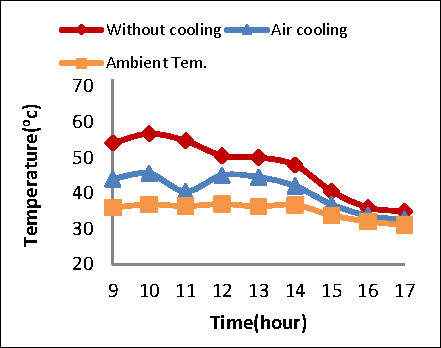
\includegraphics[width=\linewidth, trim=2 2 2 2, clip]{Figures/air_cooling_temperature_graph.pdf}
        \caption{Comparison of PV temperature when using air cooling over time \cite{Al-Masalha2024},}
        \label{fig:air_cooling_temperature_graph}
    \end{minipage}
    \hfill
    \begin{minipage}{0.45\linewidth}
        \centering
        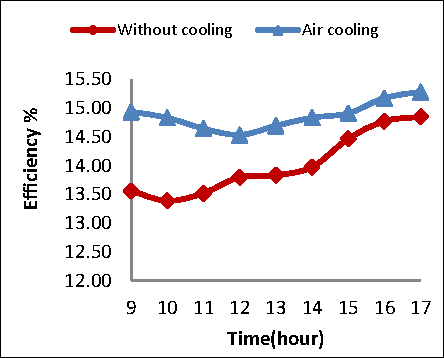
\includegraphics[width=\linewidth, trim=2 2 2 2, clip]{Figures/air_cooling_efficiency_graph.pdf}
        \caption{Comparison of efficiency when using air cooling over time \cite{Al-Masalha2024}.}
        \label{fig:air_cooling_efficiency_graph}
    \end{minipage}
\end{figure}

\textit{Water-Based Cooling Methods}\par
Al-Masalha et al.’s water cooling method involved spraying water directly onto the photovoltaic modules to dissipate heat. As illustrated in Figure \ref{fig:water_cooling_temperature_graph}, this technique resulted in a temperature reduction of the photovoltaic module ranging from 20.45\% to 35.44\%. Consequently, as shown in Figure \ref{fig:water_cooling_efficiency_graph}, this temperature reduction led to an efficiency improvement between 0.6\% and 1.8\% \cite{Al-Masalha2024}.

\begin{figure}[H]
    \centering
    \begin{minipage}{0.45\linewidth}
        \centering
        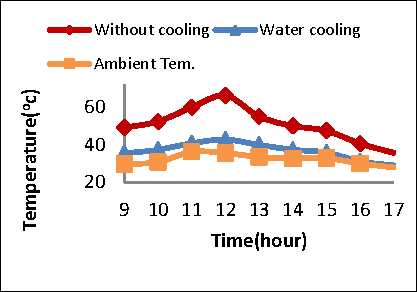
\includegraphics[width=\linewidth, trim=2 2 2 2, clip]{Figures/water_cooling_temperature_graph.pdf}
        \caption{Comparison of PV temperature when using water sprinklers over time \cite{Al-Masalha2024}.}
        \label{fig:water_cooling_temperature_graph}
        \vspace{-2em}
    \end{minipage}
    \hfill
    \begin{minipage}{0.45\linewidth}
        \centering
        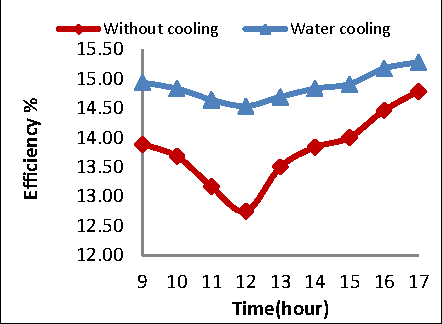
\includegraphics[width=\linewidth, trim=2 2 2 2, clip]{Figures/water_cooling_efficiency_graph.pdf}
        \caption{Comparison of efficiency when using water sprinklers over time \cite{Al-Masalha2024}.}
        \label{fig:water_cooling_efficiency_graph}
        \vspace{-2em}
    \end{minipage}
\end{figure}

\textit{Hybrid Cooling Methods}\par
In their final approach, Al-Masalha’s team developed a hybrid cooling system by combining water spraying and air-cooling techniques. This integrated method produced the most significant results in terms of both temperature reduction and efficiency improvement. The hybrid cooling system achieved a temperature reduction in the range of 30\% and 40\%, shown in Figure \ref{fig:hybrid_cooling_temperature_graph}. This substantial reduction in temperature led to an increase in photovoltaic module efficiency, ranging from 0.88\% to 2\%, as illustrated in Figure \ref{fig:hybrid_cooling_efficiency_graph} \cite{Al-Masalha2024}.\vspace{1em}

\begin{figure}[H]
    \centering
    \begin{minipage}{0.45\linewidth}
        \vspace{-1em}
        \centering
        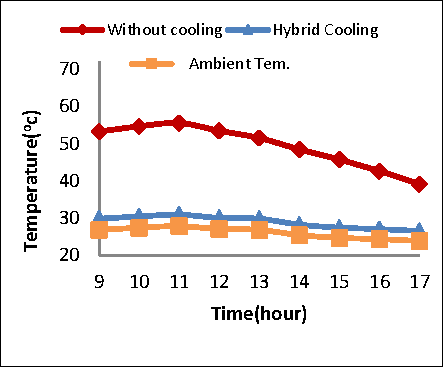
\includegraphics[width=\linewidth, trim=2 2 2 2, clip]{Figures/hybrid_cooling_temperature_graph.pdf}
        \vspace{-3.5em}
        \caption{Comparison of PV temperature when using hybrid cooling over time \cite{Al-Masalha2024}.}
        \label{fig:hybrid_cooling_temperature_graph}
    \end{minipage}
    \hfill
    \begin{minipage}{0.45\linewidth}
        \vspace{-0.5em}
        \centering
        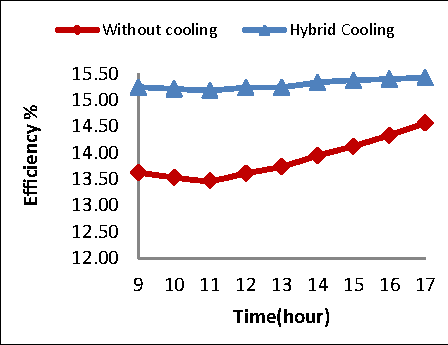
\includegraphics[width=\linewidth, trim=2 2 2 2, clip]{Figures/hybrid_cooling_efficiency_graph.pdf}
        \vspace{-2.5em}
        \caption{Comparison of efficiency when using hybrid cooling over time \cite{Al-Masalha2024}.}
        \label{fig:hybrid_cooling_efficiency_graph}
    \end{minipage}
\end{figure}\vspace{-1em}

\textit{Nano-fluid Based Cooling Methods}\par
In recent times, nanofluid-based cooling methods have emerged as a highly effective technique for enhancing the thermal management and overall efficiency of photovoltaic modules. In 2022, T.K. Murtadha et al. conducted an experimental investigation into the performance enhancement of photovoltaic modules using titanium dioxide nanofluids. Their findings indicated that higher nanoparticle concentrations correlated with improved heat dissipation, resulting in a maximum efficiency gain of 19.23\% under optimal nanofluid cooling conditions \cite{Murtadha2022}.

\textit{An Assessment and Conclusion on the Most Promising Cooling Method}\par
The studies conducted by Al-Masalha et al. \cite{Al-Masalha2024} and Murtadha et al. \cite{Murtadha2022} clearly demonstrate that water and nanofluid cooling methods outperform air-based cooling in terms of thermal regulation and efficiency improvement for photovoltaic modules. However, despite their superior performance, water and nanofluid cooling systems are significantly less prevalent than air cooling in photovoltaic applications. This disparity is primarily due to several practical limitations. Both water and nanofluid systems entail higher initial and operational costs, as well as increased system complexity \cite{Dwivedi2020, Suresh2018}. Additionally, they demand more frequent and intensive maintenance compared to air cooling systems, further escalating long-term expenses \cite{Samykano2023, Ponticorvo2022}. Moreover, the structural load associated with liquid- based cooling is greater due to the added weight of the coolant medium, which imposes additional design and material constraints \cite{Sakanova2016}. These factors collectively impact the cost-effectiveness of photovoltaic cooling strategies, rendering air cooling the most viable option for both commercial and residential implementations. Consequently, air cooling remains the most employed method for photovoltaic module thermal management \cite{Dwivedi2020}.\par

As was stated previously, Al-Masalha et al. implemented active cooling of photovoltaic modules using electric powered air fans to facilitate convective heat transfer \cite{Al-Masalha2024}. However, this approach incurs a parasitic energy cost, as external power is required to operate the fans. Vortex generators provide a passive cooling alternative that uses wind to induce localised turbulence and enhance convective heat transfer. Therefore, the following section explores the use of vortex generators to enhance the thermal management of photovoltaic modules.

\subsection{Vortex Generators}
Vortex generators are protrusions on a heat transfer surface that induce swirling flow around an axis, generating vortices that enhance convective heat transfer \cite{Awais2018}. Figure \ref{fig:vortex_generator} illustrates this phenomenon for a cylindrical vortex generator interacting with the surrounding fluid.
\vspace{-1em}
\begin{figure}[H]
    \centering
    \includegraphics[width=\linewidth]{Figures/vortex_generator.pdf}
    \vspace{-2em}
    \caption{Fluid flow over a cylinder. Adapted from \cite{VanTreuren2015}.}
    \label{fig:vortex_generator}
\end{figure}
\vspace{-1.5em}

Figure \ref{fig:vortex_generator} also draws attention to two key features associated with vortex generators: the forward stagnation point and the separation point. At the forward stagnation point, the fluid velocity, $u$, is zero, while the separation point marks the location where the airflow detaches from the surface of the object. At the separation point, vortices, referred to as Kármán vortices in the context of cylindrical bodies, are generated \cite{Wille1960}. These vortices promote mixing between the high-momentum outer fluid and the low-momentum near-wall fluid, enhancing momentum and energy exchange near the surface. This mixing thins the thermal boundary layer, thereby enhancing convective heat transfer as previously discussed. Section 2.4.1 presents the theoretical basis for the described flow behaviour.\par

\subsubsection{Vortex Generators: A Theoretical Confirmation}
The location of the separation point on a cylinder depends on the boundary layer’s transition from laminar to turbulent flow. This transition is primarily characterised by the Reynolds number, $\mathrm{Re}$, defined as the 
ratio of inertial to viscous forces in the fluid. For cylindrical shapes, the Reynolds number is found using Equation 14 \cite{engel2014ExternalForcedConvection}.
\begin{equation}
    \mathrm{Re_D} = \frac{\rho VD}{\mu} = \frac{VD}{\nu}
\end{equation}
The Reynolds number is closely related to the Nusselt number; however, for cylindrical vortex generators in cross flow, the relationship is not straightforward. To address this, Churchill and Bernstein (1977) proposed an empirical correlation to estimate the average Nusselt number for cross flow over a cylinder, $\mathrm{Nu_{cyl}}$, incorporating both the Reynolds and Prandtl numbers, as shown in Equation 15 \cite{engel2014ExternalForcedConvection}.
\begin{equation}
    \mathrm{Nu_{cyl}} = 0.3 + \frac{0.62 \mathrm{Re^{\frac{1}{2}}Pr^{\frac{1}{3}}}}{[1+(\frac{0.4}{\mathrm{Pr}})^{\frac{2}{3}}]^{\frac{1}{4}}}[1+(\frac{\mathrm{Re}}{282,000})^{\frac{5}{8}}]^{\frac{4}{5}}
\end{equation}
The average Nusselt number, $\mathrm{Nu_{cyl}}$, has a proportional relationship with the average convective heat transfer coefficient, $h$, shown in Equation 16 \cite{engel2014ExternalForcedConvection}.
\begin{equation}
    \mathrm{Nu_{cyl}} = \frac{hD}{k}
\end{equation}
Thus, the resulting convective heat transfer coefficient, $h$, can be used to determine the rate of convective heat transfer, as shown in Equation 9, thereby quantifying the effect of cylindrical vortex generators on heat transfer \cite{engel2014IntroductionAndBasicConcepts}.

\subsubsection{Vortex Generator-Based Cooling Methods}
A 2024 study led by Z. Zhou from the University of New South Wales investigated the effect of vortex 
generators on photovoltaic module cooling. Zhou et al. attached rectangular wing vortex generators, 
made from either aluminium sheet or 3D-printed thermally conductive polymer, to the rear side of the 
photovoltaic modules. Although the vortex generators were optimised for free convection, both designs 
successfully reduced the photovoltaic module temperature by 1.5 \textdegree C under low wind conditions and high irradiance. In scenarios with high module temperatures and windy conditions, the aluminium vortex generators achieved a greater cooling effect, reducing the module temperature by 2.5 \textdegree C \cite{ZiboZhou2024}. Zhou et al.’s observation of variations in results due to different vortex generator materials highlights the significant influence of vortex generator parameters on photovoltaic module cooling \cite{ZiboZhou2024}. As a result, several studies have investigated the influence of other vortex generator parameter modifications on the thermal performance of photovoltaic modules.

\textbf{Effect of Vortex Generator Orientation on Photovoltaic Module Temperature Reduction}\par
A 2023 study conducted by S. Schiffman from the University of New South Wales investigated the effect of vortex generator orientation on photovoltaic module temperature.
\begin{figure}[H]
    \centering
    \begin{minipage}{0.48\linewidth}
        \centering
        \includegraphics[width=\linewidth, trim=0 10 0 10, clip]{Figures/fwd_full_formation_page-0001.jpg}
        \vspace{-2em}
        \caption{Forward facing vortex generator arrangment. Adapted from \cite{Schiffmann2023}.}
        \label{fig:fwd_full_fomation}
    \end{minipage}
    \hfill
    \begin{minipage}{0.48\linewidth}
        \centering
        \includegraphics[width=\linewidth, trim=0 10 0 10, clip]{Figures/back_full_formation_page-0001.jpg}
        \vspace{-2em}
        \caption{Backward facing vortex generator arrangement. Adapted from \cite{Schiffmann2023}.}
        \label{fig:back_full_formation}
    \end{minipage}
    \vspace{-1em}
\end{figure}
Schiffman positioned 3D-printed vortex generators in two configurations: a forward-facing arrangement (Figure \ref{fig:fwd_full_fomation}) and a backward-facing arrangement (Figure \ref{fig:back_full_formation}). Schiffman's experiment revealed that although both configurations enhanced cooling of the photovoltaic module, the backward-facing arrangement consistently achieved greater temperature reductions across wind speeds of $1,\text{m/s}$, $2,\text{m/s}$, and $3,\text{m/s}$. Specifically, the backward-facing setup achieved mean temperature reductions of approximately $1.4\ ^\circ\text{C}$, $0.75\ ^\circ\text{C}$, and $0.7\ ^\circ\text{C}$, respectively \cite{Schiffmann2023}.

\textbf{Effect of Vortex Generator Shape on Photovoltaic Module Temperature Reduction}\par
Schiffman's results and experimental setup laid the foundation for further investigations into additional parameters influencing module cooling performance. Building on this work, I.R. Chaudhury examined the impact of vortex generator geometry on photovoltaic module cooling. Chaudhury tested several shapes, including cube, cylindrical, pyramid, inverted pyramid, and winglet configurations, shown in Figure \ref{fig:vortex_generator_shapes}. \par

\begin{wrapfigure}{r}{0.6\textwidth}
    \vspace{-2em}
    \centering
    \includegraphics[width=\linewidth, trim=0 0 0 0, clip]{Figures/vortex_generator_shapes.pdf}
    \vspace{-3em}
    \caption{VG Geometry Configurations. Adapted from \cite{Chaudhury2024}.}
    \label{fig:vortex_generator_shapes}
    \vspace{-2em}
\end{wrapfigure}

While winglet-shaped vortex generators reduced photovoltaic module temperature by $5\ ^\circ \text{C}$ at $1$ m/s, their free-convection based design meant that cooling effectiveness diminished at higher wind velocities. In contrast, cylindrical-shaped vortex generators demonstrated the most favourable trend, causing greater temperature reductions as the velocity increased. Thus, Chaudhury encouraged the selection of the cylindrical vortex generator for further experimentation, focusing on spacing configurations to promote turbulent flow in the stream-wise direction \cite{Chaudhury2024}.

\textbf{Effect of Vortex Generator Spacing on Photovoltaic Module Temperature Reduction}\par
\begin{wrapfigure}{r}{0.4\textwidth}
    \vspace{-2em}
    \centering
    \includegraphics[width=1\linewidth, trim=0 0 0 20, clip]{Figures/spacing_diagram.pdf}
    \vspace{-4em}
    \caption{Spacing direction of vortex generator array relative to the direction of airflow. Adapted from \cite{Zhou2024}.}
    \label{fig:spacing_diagram}
    \vspace{-4em}
\end{wrapfigure}

Consequently, in 2024, Z. Zhou investigated the effects of span-wise, $d_x$, and stream-wise, $d_y$, spacing of cylindrical vortex generators on photovoltaic module temperature reduction. The spacing direction of the vortex generator array relative to the direction of airflow is shown in Figure \ref{fig:spacing_diagram}.\par

For the span-wise spacing group, Zhou tested five values of horizontal spacing, $d_x$ ($26$ mm, $51$ mm, $102$ mm, $153$ mm, and $204$ mm), while maintaining a constant stream-wise spacing, $d_y$, of $79$ mm. Each configuration was subjected to forced convection wind speeds of $1.3$ m/s, $2.3$ m/s, and $3.3$ m/s.\par

Similarly, for the stream-wise spacing group, Zhou tested five values of vertical spacing, $d_y$ ($40$ mm, $79$ mm, $119$ mm, $158$ mm, and $198$ mm), with the span-wise spacing, $d_x$, fixed at $51$ mm. These configurations were subjected to forced convection wind speeds of $1$ m/s, $2$ m/s, and $3$ m/s.\par

The results indicated that $51$ mm span-wise spacing under a wind speed of $3.3$ m/s produced the greatest temperature reduction among the span-wise configurations, achieving a decrease of $2.15\ ^\circ\text{C}$. In the stream-wise group, a spacing of $79$ mm under a wind speed of $3$ m/s yielded the largest reduction, with a decrease of $2.51\ ^\circ\text{C}$ \cite{Zhou2024}.

\textbf{Effect of Vortex Generator Height on Heat Transfer}\par
\begin{wrapfigure}{r}{0.4\linewidth}
    \vspace{-2.1em}
    \centering
    \includegraphics[width=\linewidth]{Figures/huang_vg.png}
    \caption{Huang et. al's experimental setup diagram \cite{huang2023downstream}.}
    \label{fig:huang_vg}
    \vspace{-2em}
\end{wrapfigure}
In 2023, Y.X. Huang from National Cheng Kung University led a study investigating the downstream effects of turbulent flow past vortex generators. As illustrated in Figure \ref{fig:huang_vg}, the experimental setup employed rectangular-prism-shaped vortex generators, which were exposed to a constant wind speed, $M$, representing the Mach number.\par

Huang et al. employed pressure-sensitive paint to map the global surface patterns of flow over a flat plate in the presence of vortex generators. These patterns were examined at three different heights, defined as the ratio of the vortex generator height to the incoming boundary layer thickness: $h^* =\,$ 0.2, 0.5, and 1.0. As shown in Figure \ref{fig:huang_results_a}, Figure \ref{fig:huang_results_b}, and Figure \ref{fig:huang_results_c}, the downstream influence of the flow increased with the vortex generator height at a constant Mach number of $M = 0.83$ \cite{huang2023downstream}.\par

\begin{figure}[H]
    \centering
    \includegraphics[width=0.9\linewidth]{Figures/huang_results_a.png}
    \caption{Global surface pressure pattern for counter-rotating vane vortex generators at $M = 0.83$, $h^* = 1.0$ \cite{huang2023downstream}.}
    \label{fig:huang_results_a}
\end{figure}

\begin{figure}[H]
    \centering
    \includegraphics[width=0.9\linewidth]{Figures/huang_results_b.png}
    \caption{Global surface pressure pattern for counter-rotating vane vortex generators at $M = 0.83$, $h^* = 0.5$ \cite{huang2023downstream}.}
    \label{fig:huang_results_b}
\end{figure}

\begin{figure}[H]
    \centering
    \includegraphics[width=0.9\linewidth]{Figures/huang_results_c.png}
    \caption{Global surface pressure pattern for counter-rotating vane vortex generators at $M = 0.83$, $h^* = 0.2$ \cite{huang2023downstream}.}
    \label{fig:huang_results_c}
\end{figure}\vspace{-2em}

From these observations, Huang et al. concluded that taller vortex generators produced stronger device-induced vortices that extended further downstream. These stronger vortices intensify momentum exchange between the high- and low-momentum regions of the boundary layer, thereby reducing its thickness. A thinner boundary layer consequently enhances convective heat transfer, as discussed in Section 2.3.3.\par

\textit{The Impact of Vortex Generator Height on Convective Heat Transfer: A Theoretical Confirmation}\par
For a cylindrical vortex generator, the lateral area exposed to the airflow, $A_\mathrm{L}$ is proportional to its height, $H_\mathrm{VG}$, as shown in Equation 17.
\begin{equation}
    A_\mathrm{L} = \pi d H_\mathrm{VG}
\end{equation}
Consequently, increasing the vortex generator height, $H_\mathrm{VG}$, leads to a larger lateral area, $A_\mathrm{L}$. Substituting $A_\mathrm{L}$ for $A$ in Equation 9 shows that a larger exposed area enhances the overall convective heat transfer, $\dot{Q}_\mathrm{conv}$. Therefore, increasing the vortex generator height directly increases convective heat transfer.\par

Although both theoretical and experimental studies have examined the effect of vortex generator height on convective heat transfer, the research reviewed for this thesis did not conclusively determine how height influences the cooling of photovoltaic modules, highlighting a gap in the literature. Thus, to observe the height effects of vortex generators on the temperature reduction of photovoltaic modules, several experimental techniques should be considered during the experimental design process.

\subsection{Experimental Techniques}
\subsubsection{Infrared Technology}
Infrared thermography is a non-invasive technique that measures mid- to long-wave infrared radiation (IR) emitted by objects and translates it into spatially resolved temperature data \cite{Tattersall2016}. This technique is crucial to this thesis as it allows for the monitoring of temperature reductions in photovoltaic modules resulting from the application of cooling methods.\par

All bodies emit infrared radiation because of their temperature. The nature of this emission is governed by Planck’s law, which states that as the temperature of a body, $T_b$, increases, the intensity of radiation emitted, $E_{b\lambda}$, at all wavelengths also increases. This relation is expressed in Equation 18 \cite{engel2014FundamentalsofThermalRadiation}.
\begin{equation}
    E_{b\lambda}(\lambda,T_b)=\frac{C_1}{\lambda^5[\text{exp}(\frac{C_2}{\lambda T_b})-1]}
\end{equation}
Thermal imaging cameras capture the emitted radiation using an infrared detector. The infrared detector then converts the radiation into an electrical signal. The most common type of infrared detector is the micro-bolometer, consisting of a grid of tiny sensors that measure the infrared radiation from each pixel in the scene. Each sensor element changes its electrical resistance based on the amount of radiation it absorbs. The raw data is processed and transformed into a thermal image, which is displayed on a screen. A key advantage of infrared thermography is its non-contact nature which prevents any disturbance to the heat transfer process, ensuring that measurements remain accurate and reliable. This is particularly important in dynamic or sensitive environments where contact-based methods could alter the conditions being observed. Therefore, infrared thermography is a useful experimental technique that will play a key role in this 
thesis’ investigation of cooling methods for photovoltaic modules \cite{HistoryofSimpleThings2024}.

\subsubsection{Thermocouple Sensors}
A thermocouple can be defined as a sensor used to measure temperature. In a thermocouple, two wires made from different metals are joined together at both ends. One of the ends is then heated, creating a continuous current that flows in the thermoelectric circuit. If the circuit is broken at the centre, the voltage 
across the open ends, known as the Seebeck voltage, can be measured. Since the voltage changes with temperature, the Seebeck voltage can be used to determine the temperature \cite{OmegaEngineeringThermocouplesEngineering}.\par

Several types of thermocouples are available, each categorised by their specific temperature range. Among these, the K-type thermocouple is the most widely used, with a temperature range of -200 \textdegree C to 1260 \textdegree C \cite{TheEngineeringMindset2020}. The broad temperature range of the K-type thermocouple enhances its versatility across a wide variety of applications. Furthermore, its relatively low-cost materials like nickel-chromium and nickel-aluminium make it a more economical choice compared to other thermocouple types. Although the standard tolerance for a K-type thermocouple is $\pm$0.75\% within the temperature range of 0 \textdegree C to 200 \textdegree C, it remains well-suited for general-purpose temperature measurements \cite{ETWInternational2024}. Thus, the K-type thermocouple serves as an important experimental technique for measuring temperature reductions in photovoltaic modules.

\subsubsection{Particle Image Velocimetry}
\begin{wrapfigure}{r}{0.6\textwidth} % r=right, l=left; change width as needed
  \centering
  \vspace{-5.6em}
  \includegraphics[width=\linewidth]{Figures/piv_diagram.pdf}
  \vspace{-1.75em}
  \caption{Experimental arrangement for planar 2C-2D PIV in a wind tunnel. Adapted from \cite{Raffel2018}.}
  \label{fig:piv_diagram}
  \vspace{-3em}
\end{wrapfigure}
Particle Image Velocimetry (PIV) is an optical measurement technique where the velocity field of an entire region within the flow is measured simultaneously \cite{Atkins2016}. Figure 26 details a typical experimental set-up of a PIV system.\par

The process begins with the introduction of tracer particles into the flow, a procedure commonly referred to as seeding. These particles are then illuminated within a plane or volume of the flow at least twice, separated by a short and known time interval. During these illuminations, a high-speed camera captures the light scattered by the tracer particles. The captured images are divided into small regions, known as interrogation windows. Within each window, the displacement of the particle pattern between the first and second images is analysed using a cross-correlation algorithm. By calculating the particle displacement, the velocity vector at each point can be determined, resulting 
in a comprehensive velocity field \cite{Raffel2018}.\par

The use of PIV in investigating forced convection cooling methods for photovoltaic modules would be highly beneficial. PIV enables the visualisation of flow patterns, making it possible to identify stagnant regions where airflow is inadequate. This information can help optimise the experimental rig for better airflow performance. Furthermore, PIV reveals how objects within the wind tunnel, such as thermocouple probes and wind speed sensors, affect the flow patterns, offering insight into their effect on the photovoltaic system.

\subsubsection{Anemometry}
Anemometry, the measurement of airflow velocity, is a fundamental technique in experimental fluid dynamics \cite{sciencedirect_anemometry}. Wind speed can be determined using a range of physical principles, including thermal methods such as hot-wire anemometry and mechanical approaches like vane anemometry. In the context of photovoltaic systems, wind plays a critical role in heat dissipation, and variations in wind speed can influence the operating temperature of photovoltaic modules. Given the focus on the impact of vortex generators on photovoltaic module temperature, accurate measurement and control of wind conditions are therefore essential to ensure the validity of experimental results.

\textbf{Vane Anemometer}\par
Vane anemometry is a mechanical method for measuring airflow velocity. The device operates using a set of small blades mounted on an axis. As air flows through the device, the blades begin to spin, and the rotational speed is measured by a connected sensor, typically in revolutions per minute. This measurement is converted into an electrical signal and expressed in metres per second \cite{Chen_et_al_2003}. 

\textbf{Hot Wire Anemometer}\par
Hot-wire anemometry is a thermal-based approach to measuring airflow velocity. The device consists of a wire that is electrically heated above ambient temperature, creating a temperature difference between the sensor and surrounding air. As wind travels through the anemometer, forced convection heat transfer occurs, resulting in the cooling of the sensor element. The relationship between the cooling rate and air velocity is exploited through the appropriate calibration of the anemometer, allowing for the accurate measurement of wind speed \cite{Terndrup2006Available}.

\subsubsection{Computational Fluid Dynamics Modelling}
Computational Fluid Dynamics (CFD) is the process of using computers to predict liquid and gas flows based on the governing equations of conservation of mass, momentum, and energy. The CFD process requires setting up a physical problem in the form of geometrical parameters, fluid properties, and boundary conditions. The fluid domain is divided into a finite number of small elements, usually referred to as a mesh. Numerical methods are employed to solve the governing equations on the mesh. Following the setup of the governing equations, the initial conditions, boundary conditions, and solver parameters are specified. Iterative computation is then performed to calculate flow variables, and the procedure is followed iteratively until the convergence is achieved. Subsequently, the results can be analysed and significant data such as flow patterns, pressure distribution, and temperature fields can be visualised. CFD modelling thus forms a flexible instrument for the validation of experimental data and mathematical models, and hence forms an important technique to be considered while determining the impact of vortex generators on photovoltaic module temperature \cite{ansys_cfd_2025}.

\subsection{Literature Gap}
The literature review in this paper initially outlined the principles governing photovoltaic modules and subsequently addressed their performance limitations. In particular, the review explored the reduction in energy conversion efficiency of photovoltaic modules at elevated temperatures.\par

Several conductive, radiative, and convective heat transfer methods aimed at reducing the temperature of photovoltaic modules were discussed. Of these different modes of heat transfer, convection had the greatest impact on module temperature, as most of the heat dissipation occurred through convective mechanisms. Thus, an in-depth investigation into natural and forced convective cooling methods for photovoltaic modules was undertaken, with the literature review concluding that forced convection is more effective at reducing module temperature than natural convection.\par

In accordance with this conclusion, several air-, water- and nanofluid-based forced convection cooling methods were examined. While it was determined that water- and nanofluid-based cooling methods outperformed air-based cooling methods, the limitations of liquid-based cooling methods in the context of photovoltaic modules could not be overlooked. The higher initial and operational costs, increased system complexity, increased maintenance requirements and higher structural load associated with liquid-based cooling methods made air-based cooling the more realistic option for photovoltaic systems. Of the air-based cooling methods examined, vortex generators were particularly notable due to their passive cooling capability, eliminating the need for external power input as would be required with active methods such as air fans. Thus, an exploration into the effectiveness of vortex generators in cooling photovoltaic modules was conducted.\par

Prior to this thesis, students at the University of New South Wales investigated the effects of vortex generators on photovoltaic module temperature reduction, with each study focusing on a different parameter related to the vortex generator. Optimal orientation, shape and spacing of vortex generators were examined under forced convection conditions. Through extensive review of these papers, in addition to other investigations into vortex generator-based cooling methods, it was determined that a lack of understanding surrounding the optimal height of vortex generators in the context of photovoltaic module temperature reduction was evident. Therefore, this thesis will focus on investigating the relationship between vortex generator height and the reduction of photovoltaic module temperature under forced convection conditions.\par

The aims of this thesis are expressed as follows:
\begin{enumerate}
    \renewcommand{\labelenumi}{\Roman{enumi}.}
    \item Confirm existing results surrounding the ability of cylindrical vortex generators to reduce the temperature of photovoltaic modules.
    \item Identify the optimal vortex generator height required to induce the largest reduction in photovoltaic module temperature and consequently, the greatest increase in the electrical efficiency of the module.
    \item Further refine the experimental testing procedure to improve its overall accuracy, repeatability, and suitability for evaluating vortex-generator performance.
\end{enumerate}

\pagebreak
\section{Methodology}
\begin{comment}
In this section you are expected to present your methodology: the tools you have used and the way in which you have applied them, with proper reference to literature sources when required. This includes both theoretical and experimental methods included in your research. Highlight the main methodological novelty/challenges of your work and try to present your methodology in a clear way, possibly using graphical devices such as flowcharts or block diagrams.
    
This section should be indicatively \textbf{~10-15 pages}. Remember to reference properly any material that you obtain from literature or other sources.
\end{comment}
\subsection{Overview of Experimentation}
The aims of this thesis, as outlined in Section 2.6, were addressed using an experimental methodology that builds directly on the work of previous thesis students, whose contributions laid the foundation for this research: Z. Zhou \cite{Zhou2024}, I.R. Chaudhury \cite{Chaudhury2024}, and S. Schiffmann \cite{Schiffmann2023}. The following procedure outlines the approach taken to achieve these aims.
\begin{enumerate}
    \renewcommand{\labelenumi}{\Roman{enumi}.}
    \item Based on experimental testing conducted by Chaudhury et al., an optimal vortex generator shape was selected from five variations: winglet, cube, cylinder, pyramid, and inverted pyramid according to their geometric characteristics and cooling performance under forced convection conditions \cite{Chaudhury2024}. Then, based on the experimental campaign conducted by Zhou et al., an optimal vortex generator spacing configuration was selected from the following options: (25.5 × 79) mm, (51 × 79) mm, (102 × 79) mm, (153 × 79) mm, (204 × 79) mm, (51 × 39.5) mm, (51 × 118.5) mm, (51 × 158) mm, and (51 × 197) mm \cite{Zhou2024}. An explanation of both choices can be found in Section 2.4.2.
    \item Following the selection of the optimal vortex generator shape and spacing arrangement, the heights to be tested were determined. An explanation for choice of vortex generator heights can be found in Section 3.3.1. These heights, along with the selected shape and spacing, resulted in a configuration previously examined by Chaudhury et al. and Zhou et al. This allowed the replication of their experimental tests and provided a solid foundation for the present study.
    \item Once previous tests were replicated and any discrepancies between the experimental results of this study and those of past thesis students were explained, vortex generator arrays of varying heights were tested to identify the optimal height for reducing photovoltaic module temperature. The data collected from these tests was then processed using FLIR and MATLAB, to calculate the temperature difference between the vortex generator test case and the existent baseline model. These results were then plotted to show the temperature difference across different vortex generator heights at wind speeds of 1, 2, and 3 m/s.
\end{enumerate}

\pagebreak

\subsection{Experimental Equipment}
This section of the report outlines the equipment used in the experimental process and their application.\par
\textbf{Photovoltaic Module}\par
To observe the effects of vortex generators on photovoltaic module temperature reduction, a standard photovoltaic module was used during experimentation. The photovoltaic module that was used was the WINAICO Perc Series P6 WST-285P6 PV module \cite{winaico_wst_285p6}, whose properties can be found in Table \ref{tab:pv_module_properties}. Infrared images of the photovoltaic module were captured throughout the experimental testing process and compared to assess temperature variations resulting from the presence of vortex generators.
\begin{table}[H]
    \centering
    \caption{WINAICO Perc Series P6 WST-285P6 PV Module Properties \cite{winaico_wst_285p6}}
    \begin{tabularx}{\textwidth}{l X} % two columns: property + details
        \toprule
        \textbf{Properties} & \textbf{Details} \\
        \midrule
        Material & Polycrystalline silicon \\
        Frame material & Black anodised aluminium \\
        Dimensions & 1665 mm length, 999 mm width, 35 mm depth \\
        Cells & Total 60; 10 cells long, 6 cells wide \\
        Rated power & Total 285 W; 4.75 W per cell \\
        Open circuit voltage/current & 38.9 V / 9.57 A \\
        Maximum series fuse & 25 A \\
        Efficiency rating & 17.13 \% under STP; solar irradiation 1,000 W/m\textsuperscript{2}, light spectrum AM 1.5, operating temperature 25$^\circ$C \\
        Electricity output decline & Year 1: 3.0 \%, Years 2--25: 0.7 \% \\
        Temperature coefficient of $P_\text{max}$ & -0.43 \%/$^\circ$C \\
        Temperature coefficient of $V_\text{oc}$ & -0.33 \%/$^\circ$C \\
        \bottomrule
    \end{tabularx}
    \label{tab:pv_module_properties}
\end{table}

\textbf{Large Wind Tunnel}\par
\begin{wrapfigure}{r}{0.55\textwidth}
    \centering
    \vspace{-1.35em}
    \includegraphics[width=0.55\textwidth]{Figures/replace_unsw_LWT.png}
    \caption{UNSW Large Aerodynamics Wind Tunnel \cite{UNSWFlowNoiseGroup}.}
    \label{fig:large_wind_tunnel}
    \vspace{-1em}
\end{wrapfigure}

The UNSW large aerodynamic wind tunnel (LWT) is a low turbulence, closed return wind tunnel that supports aerodynamic and wind engineering research, shown in Figure \ref{fig:large_wind_tunnel}. The LWT has a small test section with a rectangular cross section measuring 1.22 m in width by 0.91 m in height. Furthermore, the small test section allows an operating flow velocity of 5 to 60 m/s and a low turbulence intensity of 0.1\%. The LWT also has a large test section with a regular octagon cross section. The cross section has a height of 3.05 m, a cross sectional area of 7.70 $\mathrm{m}^2$, and an operating flow velocity of 0.72 to 8.65 m/s. In addition, the large test section of the LWT accommodates hot-wire anemometry, allowing wind speed measurements to be monitored and, when necessary, corrected during testing, resulting in increased accuracy \cite{UNSWFlowNoiseGroup}. Moreover, the large test section of the LWT allows the photovoltaic module (detailed in Table \ref{tab:pv_module_properties}) to be fully enclosed within the wind tunnel during testing, ensuring that the results reflect real-world conditions without interference from tunnel edges, pressure gradients, or incomplete flow interactions. Thus, to simulate forced convection conditions, experimental testing was conducted in the large test section of the LWT.\par

\textbf{Junction Box and DC 1.2 kW Power Supply (QPX1200SP)}\par
\begin{wrapfigure}{r}{0.35\textwidth}
    \vspace{-1.25em}
    \centering
    \includegraphics[width=1\linewidth]{Figures/junction_box.jpg}
    \caption{Junction Box \cite{aimtti_qpx1200sp}}
    \vspace{-0.5em}
    \label{fig:junction_box}
\end{wrapfigure}

The junction box (Figure \ref{fig:junction_box}) and 1.2 kW DC power supply were used to heat the photovoltaic module, simulating its operating temperature under sunny outdoor conditions \cite{aimtti_qpx1200sp}. A 2023 study by Y.A. Rahman reported that photovoltaic modules typically reach around 45 \textdegree C in such conditions \cite{Rahman.2023}. To replicate this, the voltage of the DC power supply was initially set to 30 V, allowing current to flow through the junction box before increasing the output to 50 V. Prior error analysis conducted by Zhou et al. indicated that voltage and current delivery errors range from 0.1 to 0.3\% \cite{Zhou2024}. Once the power supply stabilised, the voltage was adjusted to approximately 44 V, which raised the photovoltaic module temperature to approximately 45 \textdegree C.\par

\textbf{Acrylic Sheets To Simulate Roofing}\par
In practice, photovoltaic modules are typically mounted on roofing. To replicate this configuration, acrylic sheets were positioned directly beneath the module to simulate the roofing structure. The acrylic roofing was divided into three sections to facilitate assembly and disassembly, which was necessary for installing vortex generators on the underside of the photovoltaic module.\par

\textbf{Acrylic Sheets To Facilitate Unidirectional Flow}\par
To replicate the conditions of a photovoltaic module installed on a household roof, unidirectional airflow was required such that air entering the space between the photovoltaic module and the acrylic roof passed through the vortex generator array before exiting. Allowing airflow to escape laterally from this space would have generated unwanted turbulence, which would compromise the validity of the tests. To prevent this, acrylic side panels were installed on either side of the photovoltaic module to enforce unidirectional flow. The panels incorporated magnetic tape, allowing for easy assembly and disassembly. Moreover, the use of acrylic ensures transparency, which was required for PIV-based experimentation.

\textbf{Support Frame}\par
The photovoltaic module and acrylic sheets were held in place by an aluminium support frame. The support frame, supplied by MayTec, was assembled to position the photovoltaic module at a 45\textdegree\, angle from the horizontal axis, in accordance with NOCT testing standards \cite{InternationalElectrotechnicalCommission2005}. The support frame was equipped with six wheels, providing enhanced manoeuvrability in the event that a critical component, such as the photovoltaic module, needed to be replaced.\par

\textbf{Hot Wire Anemometer}\par
\begin{wrapfigure}{r}{0.35\textwidth}
    \vspace{-5.15em}
    \centering
    \includegraphics[width=0.25\textwidth]{Figures/hot_wire_anemometer.png}
    \caption{Hot Wire Anemometer \cite{Testo_405_NTC}}
    \vspace{-2em}
    \label{fig:hot_wire_anemometer}
\end{wrapfigure}

A hot wire anemometer consists of a small wire heated by an electric current and positioned in the air or gas stream whose velocity is to be measured \cite{ScienceDirectHotWireAnemometer}. This instrument was the primary tool used to determine wind speed due to its accuracy, reliability, and proximity to the photovoltaic module. It was inserted in front of the module through a specially designed opening in the LWT (Figure \ref{fig:hot_wire_anemometer}) to minimise airflow obstruction, enabling wind speed measurements to be taken from outside the wind tunnel.\par

\textbf{Vane Anemometer}\par
\begin{wrapfigure}{r}{0.35\textwidth}
    \vspace{-2em}
    \centering
    \includegraphics[width=0.20\textwidth]{Figures/vane_anemometer.png}
    \caption{Vane Anemometer \cite{TSI_LCA501_Vane_Anemometer_TradeIndia}}
    \label{fig:vane_anemometer}
\end{wrapfigure}

A vane anemometer measures the average velocity of airflow using rotating vanes, with the rotation speed corresponding to the flow speed. Its accuracy depends on the vane angle relative to the airflow and requires a minimum threshold velocity for operation \cite{ScienceDirectVaneAnemometer}. During testing, it was positioned ahead of the photovoltaic module in a similar manner to the hot wire anemometer but on the opposite side (Figure \ref{fig:vane_anemometer}). The instrument served as a secondary wind speed sensor to prevent a single point of failure during wind speed adjustments.\par

\textbf{Tripod}\par
\begin{wrapfigure}{r}{0.35\textwidth}
    \vspace{-4.25em}
    \centering
    \includegraphics[width=0.15\textwidth]{Figures/tripod.png}
    \caption{Tripod \cite{TSI_LCA501_Vane_Anemometer_TradeIndia}}
    \vspace{-3em}
    \label{fig:tripod_image}
\end{wrapfigure}
A tripod was used to elevate the infrared camera to maintain a perpendicular distance of two metres from the photovoltaic module, as shown in Figure \ref{fig:tripod_image}. This setup followed previous experimental configurations and ensured that the entire photovoltaic module remained within the camera frame.

\textbf{FLIR E95 Thermal Imaging Camera \& Charging Cable}\par
\begin{wrapfigure}{r}{0.35\textwidth}
    \vspace{-2.5em}
    \centering
    \includegraphics[width=0.20\textwidth]{Figures/flir_e95.png}
    \caption{FLIR E95 \cite{FLIR_E95}}
    \label{fig:flir_e95}
\end{wrapfigure}
The FLIR E95 infrared camera (Figure \ref{fig:flir_e95}) was used to detect and capture the thermal energy emitted by the photovoltaic module during experimental testing, allowing assessment of the effect of vortex generators on module temperature reduction. The camera had a resolution of 348 × 464 pixels, capturing 161,472 temperature points per image. Thus, thermal images of the photovoltaic module, captured using the FLIR E95 infrared camera, were analysed to assess temperature variations caused by the presence of vortex generators.

\textbf{Zip Ties}\par
\begin{wrapfigure}{r}{0.35\textwidth}
  \vspace{-3.6em}
  \centering
  \includegraphics[trim=0 120 0 150,clip,width=0.175\textwidth]{Figures/ziptie_charger.png}
  \caption{Zip Ties}
  \label{fig:ziptie_charger}
\end{wrapfigure}

It was discovered through practical experimentation that the battery life of the FLIR infrared camera lasted approximately two hours. Due to the four hour duration of one experimental test, the infrared camera needed to be connected to its charging cable during testing. To prevent cable entanglement and minimise turbulence from the charging cable, zip ties were used to secure it to the tripod, as shown in Figure \ref{fig:ziptie_charger}.\par

\textbf{Masking Tape}\par
\begin{wrapfigure}{r}{0.35\textwidth}
  \vspace{-3.45em}
  \centering
    \includegraphics[trim=0 0 0 0,clip,width=0.25\textwidth,height=2cm]{Figures/masking_tape_tripod.png}
  \vspace{-0.5em}
  \caption{Tripod Placement}
  \label{fig:masking_tape_tripod}
\end{wrapfigure}

As detailed in Section 4.1, the tripod position was found to influence the experimental results. To ensure consistent placement across all tests and improve repeatability, masking tape was used to mark and secure the tripod position, as shown in Figure \ref{fig:masking_tape_tripod}.

\textbf{Vortex Generators}\par
The primary objective of this thesis was to evaluate the effect of vortex generator height on the reduction of photovoltaic module temperature. Thus, an array of vortex generators (Figure \ref{fig:spacing_config}) were positioned on the underside of the photovoltaic module during experimental testing.

\textbf{Blu Tack}\par
\begin{wrapfigure}{r}{0.35\textwidth}
  \vspace{-9.95em}
  \centering
  \includegraphics[trim=100 150 100 150,clip,width=0.35\textwidth]{Figures/bluetack.png}
  \vspace{-7.5em}
  \caption{Vortex generator with Blu Tack applied.}
  \label{fig:bluetack}
\end{wrapfigure}

Blu Tack was used to attach the vortex generators to the underside of the photovoltaic module, as shown in Figure \ref{fig:bluetack}. Blu Tack was used instead of permanent adhesives such as hot glue, as it allowed the vortex generators to be repositioned to test different heights on the same photovoltaic module. Blu Tack was also selected over more discreet alternatives, such as sticky tape, as previous thesis students reported adhesion issues with tape that led to vortex generators detaching from the underside of the photovoltaic module during testing.

\textbf{Thermocouples and Resistance-to-digital converter (MAX31865)}\par
\begin{wrapfigure}{r}{0.40\textwidth}
  \vspace{-1em}
  \centering
  \includegraphics[trim=0 30 0 435,clip,width=0.40\textwidth]{Figures/thermocouple_position.png}
  \caption{Thermocouple Positions}
  \label{fig:thermocouple_position}
\end{wrapfigure}
K-type thermocouples were used to record the ambient temperature of the LWT and the photovoltaic module during experimental testing, as shown in Figure \ref{fig:thermocouple_position}. The thermocouple used to measure ambient temperature was cross-referenced with the vane and hot-wire anemometer readings, thereby reducing the risk associated with a single point of failure. Similarly, the thermocouple measuring the photovoltaic module temperature was also cross-referenced with the infrared images obtained from the thermal camera to validate accuracy and detect potential sensor errors. The thermocouples were attached using Blu Tack and connected to wires leading to the resistance-to-digital converter (RTD), where the data was digitised and stored on the laptop.

\textbf{Laptop}\par
\begin{wrapfigure}{r}{0.4\textwidth}
  \vspace{-1em}
  \centering
  \includegraphics[trim=0 0 0 0,clip,width=0.40\textwidth,height=5.5cm]{Figures/coolterm_exe.png}
  \vspace{-1.8em}
  \caption{CoolTerm Application}
  \label{fig:coolterm_exe}
  \vspace{-2em}
\end{wrapfigure}

A laptop was used to record the ambient and photovoltaic module temperature readings measured by the thermocouples during the experimental process.

\textbf{CoolTerm}\par
CoolTerm is a simple serial port terminal application (no terminal emulation) to exchange data with hardware connected to serial ports such as servo controllers, robotic kits, GPS receivers, micro-controllers, etc \cite{CoolTermHelp}. In this experiment, CoolTerm, as shown in Figure \ref{fig:coolterm_exe}, was employed to record the thermocouple temperature readings in real time and to export the collected data as a text file for subsequent analysis and processing.

\textbf{FLIR}\par
FLIR Tools is a software suite developed by FLIR Systems for working with thermal imaging cameras (infrared cameras). It’s commonly used for analysing and reporting infrared images and videos. FLIR Tools was used to process the infrared images captured during the experiment and export the resulting data as a comma-separated values (CSV) file for MATLAB-based analysis.

\textbf{MATLAB}\par
MATLAB is a high-performance programming language, software platform, and an interactive environment designed for technical computing, integrating computation, visualisation, and programming \cite{MathWorksIntroMATLAB}. MATLAB was used to analyse the CSV files from FLIR Tools and determine the changes in photovoltaic module temperature caused by the vortex generators.

\subsection{Experimental Method}
The experimental equipment described in Section 3.2 is illustrated in the experimental rig diagram (Figure \ref{fig:experimental_rig_diagram}). Furthermore, the following subsections provide a detailed description of the experimental method employed in this thesis to fulfil its objectives.\vspace{2em}

\begin{figure}[H]
    \centering
    \vspace{-1em}
    \includegraphics[width=1\linewidth]{Figures/experimental_rig_diagram.pdf}
    \caption{Diagram of the experimental rig.}
    \label{fig:experimental_rig_diagram}
\end{figure}

\subsubsection{Experimental Set-up}
For each test configuration, the vortex generators must be attached to the underside of the photovoltaic module using Blu Tack. Following this, the three acrylic roof panels should be positioned directly below the photovoltaic module. Additionally, six acrylic side panels must be attached to the experimental rig to create a channel flow environment, with three panels on each side of the photovoltaic module.\par

The DC power supply must be activated to supply a regulated 44 V DC output to the photovoltaic module. Furthermore, both anemometers should be activated to ensure accurate wind speed measurements. Thermocouples should be positioned on both the acrylic roof structure and the photovoltaic module; the thermocouple on the roof records the ambient temperature, while the one on the photovoltaic module measures its temperature. To record thermocouple data to a text file, the CoolTerm.exe application must be properly configured. A complete instruction set to configure the CoolTerm.exe file can be found in Appendix C.1.\par

The tripod-mounted FLIR camera should be positioned to the side of the photovoltaic module, as shown in Figure \ref{fig:side_tripod}, to minimise airflow disruptions over the module surface caused by the tripod. The tripod height should then be adjusted so that it is two metres from the photovoltaic module (Figure \ref{fig:experimental_rig_diagram}) and the entire module is visible to the FLIR camera. The automatic image capture method, set to five-minute intervals, can then be started. This involves taking 60 photos over five hours. The five-hour duration was chosen to accommodate setup and shutdown time before and after the standard four-hour experimental test.\par

Finally, the wind tunnel must be turned on by activating the main switch, isolating switch, booster pump, and start button in that order. Once operational, the vertical wind speed switch should be turned on, and the directional flow dial set to ‘Forward’.

\textbf{Experimental Conditions and Assumptions}\par
Several assumptions were made during the experimental campaign, including uniform surface emissivity and the negligible influence of Blu Tack on flow and heat transfer characteristics.\par

A uniform emissivity value across the photovoltaic module surface was assumed to simplify radiative heat transfer analysis, as the module’s glass cover exhibits minimal spatial variation in emissivity. This assumption is common in similar experimental studies and has negligible influence on overall thermal performance compared to convective and conductive effects \cite{Chaudhury2024, Zhou2024}.\par

It was assumed that the Blu Tack used to secure the vortex generators to the underside of the panel had a negligible influence on the aerodynamic behaviour and heat transfer characteristics, as its size, placement, and material properties are unlikely to affect the dominant flow or thermal processes \cite{Zhou2024}.
\newpage

\textbf{Constant Configurations}\par
\textit{Vortex generator properties}\par
The vortex generators used in this study were cylindrical structures made from polylactic acid (PLA), each with a diameter of 20 mm, as shown in Figure \ref{fig:vg_heights_diagram}. Cylindrical vortex generators were selected over other geometries based on the experimental findings of Chaudhury et al., who evaluated the effectiveness of cube, cylindrical, pyramid, inverted pyramid, and winglet-shaped vortex generators in reducing photovoltaic module temperatures under forced convection conditions, as detailed in Section 2.4.2 \cite{Chaudhury2024}. As a result, cylindrical vortex generators identical in diameter and material to those used by Chaudhury et al. were adopted in this study. Chaudhury et al.'s results summary can be found in Appendix C.2.

\textit{Vortex generator array spacing configuration}\par
\begin{wrapfigure}{r}{0.5\textwidth}
    \vspace{-4.2em}
    \centering
\includegraphics[width=\linewidth, trim=0 15 0 17.5, clip]{Figures/spacing_config.pdf}
    \vspace{-1.5em}
    \caption{Vortex generator array spacing configuration. $d_x=51$ mm and $d_y = 79$ mm.}
    \label{fig:spacing_config}
    \vspace{-1em}
\end{wrapfigure}
The vortex generators were mounted on the underside of the photovoltaic module with a uniform span-wise spacing of 51 mm and a stream-wise spacing of 79 mm, as illustrated in Figure \ref{fig:spacing_config}. This spacing configuration was selected based on the experimental results of Zhou et al. As detailed in Section 2.4.2, Zhou et al. investigated the effects of span-wise and stream-wise spacing of cylindrical vortex generators on the reduction of photovoltaic module temperatures \cite{Zhou2024}. Zhou et al.’s results indicated that a vortex generator array with a span-wise spacing of 51 mm and a stream-wise spacing of 79 mm was the most effective in reducing module temperatures under forced convection conditions. Thus, the vortex generator array spacing was set to 51 mm by 79 mm during all experimental testing in this study. Zhou et al.'s results summary can be found in Appendix C.3.

\textit{Wind speed conditions}\par
Experimental testing was conducted in the large test section of the LWT at wind speeds of 1, 2, and 3 m/s. These speeds were chosen to align with the baseline data recorded by S. Schiffmann \cite{Schiffmann2023}, which allowed the reduction in photovoltaic module temperature to be calculated without the need to conduct additional baseline tests.

\textit{Photovoltaic module specifications}\par
The perpendicular distance between the photovoltaic module and the acrylic roofing (Figure \ref{fig:experimental_rig_diagram}) was maintained at 150 mm throughout experimental testing. Furthermore, the photovoltaic module's 45\textdegree\, angle of inclination and orientation relative to the direction of airflow was kept constant throughout the experimental campaign.

\textit{Thermal camera calibration parameters}\par
Calibration parameters, including the emissivity of the photovoltaic module surface, were kept consistent throughout the experimental campaign due to their direct relation to radiative heat transfer, as detailed in Section 2.3.2.

\textit{DC power supply}\par
Variations in the heating temperature of the photovoltaic module, induced by the DC power supply, between baseline and vortex generator test cases would render the observed temperature reductions attributable to the vortex generators unreliable. Thus, the DC power supply was operated at a constant output of 44.5 volts throughout all baseline and vortex generator experiments to ensure consistency.

\textit{Anemometer placements}\par
Consistent placement of the anemometers within the large test section of the wind tunnel was necessary to ensure that the photovoltaic module experienced uniform wind speeds across all experiments. Inconsistent placement would have influenced the measured wind speeds for two reasons: the velocity distribution within the wind tunnel is non-uniform, and the anemometers serve as reference instruments for adjusting the airflow velocity during testing.

\textit{Thermocouple placements}\par
Consistency in thermocouple placement was essential due to its proximity to the photovoltaic module. The elevated temperature of the module, relative to its surroundings as a result of DC power supply heating, can artificially increase the ambient temperature recorded when the thermocouple is positioned too close to the module. Therefore, the thermocouple used to measure ambient temperature was mounted on the acrylic roofing structure at a sufficient distance from the photovoltaic module to minimise thermal interference. To further reduce the risk of inflated ambient temperature readings, the temperature sensors integrated into both anemometers, located at substantial distances from the photovoltaic module while remaining within the wind tunnel, were employed as cross-references throughout all experiments.

\textit{Thermal camera and tripod placement}\par
As discussed in Section 4.1, variations in the position of the thermal camera and its tripod had a substantial impact on the experimental results. Specifically, when the tripod was placed directly in front of the photovoltaic module (Figure \ref{fig:centred_tripod}), it induced turbulence that lowered the module temperature and artificially increased the calculated temperature reduction. Consequently, the placement of the thermal camera and tripod affected test repeatability, as the measured temperature reductions were significantly smaller when the camera was positioned to the side (Figure \ref{fig:side_tripod}). To eliminate this source of error and ensure repeatability, the tripod and thermal camera were positioned to the side of the photovoltaic module for all experiments. In addition, the tripod leg positions were marked with duct tape to maintain consistent placement across tests, as shown in Figure \ref{fig:masking_tape_tripod}.


\textbf{Variable Configurations}\par
\textit{Vortex generator heights}\par
The main objective of this thesis was to evaluate the effect of vortex generator height on the temperature reduction of a photovoltaic module. As a result, three vortex generator heights were selected: 15 mm, 75 mm, and 150 mm. The three vortex generators can be observed in Figure \ref{fig:vg_heights_diagram}.\par

The 15 mm height was selected to enable replication of previous experimental test cases conducted by Zhou et al. and Chaudhury et al. during their respective theses. A confirmation of Zhou et al. and Chaudhury et al.'s results would establish confidence in the experimental setup and provide a validated foundation for subsequent testing of the 75 mm vortex generators and the 150 mm vortex generators. Any discrepancies between the current and previous findings would prompt an investigation to identify the source of variation. This process would, in turn, enhance the credibility of the results presented in this report. In addition, such an investigation may also reveal potential limitations in the experimental methodologies employed by Zhou et al. or Chaudhury et al.\par

\begin{wrapfigure}{r}{0.5\linewidth}
    \vspace{-2em}
    \centering
    \includegraphics[width=0.76\linewidth, trim={0 0 0 0.9cm}, clip]{Figures/vg_heights_diagram.pdf}
    \vspace{-1.60em}
    \caption{Independent variable for the study: vortex generator heights tested. All dimensions are in mm.}
    \label{fig:vg_heights_diagram}
    \vspace{-2em}
\end{wrapfigure}

The 75 mm and 150 mm vortex generator heights were selected based on the 150 mm perpendicular distance between the acrylic roofing structure and the photovoltaic module. Thus, the 75 mm vortex generators would take up 50\% of this perpendicular distance and the 150 mm vortex generators would take up 100\%. A linear relationship between vortex generator height and photovoltaic module temperature reduction could be adequately characterised using these heights alone. However, if unexpected results were observed, additional vortex generator heights within the 15–150 mm range could be tested to obtain a more comprehensive understanding of the relationship between height and temperature reduction. Thus, to discover a more optimal vortex generator height, additional heights could be tested between these limiting cases.\par

\subsubsection{Experimental Procedure}
Provided that the experimental setup described in Section 3.3.1 has been completed, the experimental test may proceed.

\textbf{Experimental Test}\par
For each test configuration, the wind speed dial must be adjusted to maintain an airflow velocity of 1 m/s across the surface of the photovoltaic module for 110 minutes to allow temperature and speed stabilisation. Between 110 and 120 minutes, three thermal images are captured at five-minute intervals using the fixed image capture method. Subsequently, the wind speed is increased to 2 m/s and maintained for 50 minutes, followed by the capture of three thermal images between 50 and 60 minutes. This procedure is then repeated a final time at 3 m/s, with a 50-minute stabilisation period and three thermal images captured during the final 10 minutes. These stabilisation periods were determined by a previous thesis student, S. Schiffmann et al., as shown in Figure \ref{fig:data_acquisition}.

\textbf{System Checks}\par
Throughout the experimental test, system checks should be conducted to verify the validity of the recorded data. The ambient temperature measured by the thermocouple can be cross-referenced with the ambient temperature readings from both anemometers to ensure validity. Additionally, adjustments made via the wind speed dial can be verified by comparing the wind speed measurements from the two anemometers.


\subsubsection{Experimental Shutdown}
After completing the experimental test phase, the wind tunnel airflow must be gradually reduced to a complete stop (0 m/s) by adjusting the wind speed dial. The directional flow dial should then be set to ‘Stop,’ and the vertical wind speed switch turned off. Following this, the wind tunnel should be powered down by pressing the stop button, then deactivating the booster pump, isolating switch, and main switch in that order. The DC power supply must be turned off to cease heating the photovoltaic module. Additionally, now that it is safe to enter the wind tunnel, the thermal camera’s automatic image capture and both anemometers should be switched off.
\begin{wrapfigure}{r}{0.5\linewidth}
    \vspace{0.65em}
    \centering
    \includegraphics[width=\linewidth, trim={0 15 0 15}, clip]{Figures/data_acquisition.png}
    \caption{The data acquisition process depending on temperature stabilisation \cite{Zhou2024}.}
    \label{fig:data_acquisition}
    \vspace{-3em}
\end{wrapfigure}
Finally, the CoolTerm.exe application can be disconnected, as all necessary data has been recorded and saved to a text file.\par

\subsubsection{Data Acquisition Process}
Due to the automatic image capture method, the nine thermal images required for data processing should be imported from the FLIR camera using the FLIR Tools mobile application once the experiment is complete. This method records thermal images of the photovoltaic module at five-minute intervals. Consequently, the nine images selected must correspond to the 10 minutes preceding each increase in wind speed, as detailed in Figure \ref{fig:data_acquisition}. Additionally, the CoolTerm text file containing thermocouple data (Figure \ref{fig:coolterm_exe}) is already available on the laptop used during the experimental test.

\subsection{Data Processing}
To detail the data processing steps observed in Figure \ref{fig:data_processing_overview}, this section uses experimental data from the 15 mm vortex generator experiment conducted on August 12, 2025.
\begin{figure}[H]
    \centering
    \includegraphics[width=1\linewidth]{Figures/data_processing_overview.pdf}
    \caption{An overview of the steps involved in processing experimental data.}
    \label{fig:data_processing_overview}
\end{figure}\vspace{-2em}
\subsubsection{FLIR Processing}
The nine infrared images captured during the experiment must be imported from the FLIR camera into FLIR Tools. The steps outlined in the following subsections should then be applied to each of these images.\par

\textbf{Emissivity Configuration}\par
In FLIR Tools, the default emissivity value is set at 0.98. The emissivity value must be changed to 0.89, a value that was obtained by integrating the simulated spectral reflectance curve at a
normal incident angle over the wavelength range of 7.5 - 14 micrometres (spectral range of the camera) \cite{ZiboZhou2024}, as shown in Table \ref{tab:thermal_image_metadata}.
\begin{figure}[H]
    \centering
    \begin{minipage}[t]{0.345\textwidth}
        \centering
        \includegraphics[width=\linewidth]{Figures/IR_12-08-2025_1ms1.jpg}
        \caption{Thermal Image: $\text{IR\_12-08-2025\_1ms1}$}
        \label{fig:IR_12-08-2025_1ms1}
    \end{minipage}
    \hfill
    \begin{minipage}[t]{0.55\textwidth}
        \centering
        \vspace{-23.375em}
        \captionof{table}{Thermal image metadata extracted from FLIR Tools: $\text{IR\_12-08-2025\_1ms1}$}
        \begin{tabular}{ll}
            \toprule
            \textbf{Parameters} & \\
            \midrule
            Emissivity & \sout{0.98} 0.89 \\
            Refl. temp. & \sout{25.0 \textdegree C} 19.8 \textdegree C\\
            \addlinespace

            \textbf{Text annotations} & \\
            \midrule
            Add row & \\
            \addlinespace

            \textbf{Image Information} & \\
            \midrule
            Camera model & FLIR E95 \\
            Camera serial & 78509326 \\
            Lens & FOL 10 mm \\
            IR resolution & 348 x 464 \\
            File size & 442.7 KB \\
            Date created & 12/08/2025 12:34:24 PM \\
            Last modified & 14/08/2025 9:19:26 AM \\
            \bottomrule
        \end{tabular}
        \label{tab:thermal_image_metadata}
    \end{minipage}
\end{figure}

\textbf{Reflective Temperature Configuration}\par
\begin{wraptable}{R}{0.55\textwidth}
\vspace{-1.7em}
\centering
\caption{Thermocouple Reflective Temperature Measurements at 2025-08-12 12:34}
\begin{tabular}{ll}
\toprule
\textbf{Timestamp} & \textbf{Refl. temp. (°C)} \\
\midrule
2025-08-12 12:34:01 & 19.89 \\
2025-08-12 12:34:07 & 19.85 \\
2025-08-12 12:34:13 & 19.82 \\
2025-08-12 12:34:18 & 19.82 \\
2025-08-12 12:34:24 & 19.85 \\
2025-08-12 12:34:30 & 19.85 \\
2025-08-12 12:34:36 & 19.82 \\
2025-08-12 12:34:41 & 19.82 \\
2025-08-12 12:34:47 & 19.85 \\
2025-08-12 12:34:53 & 19.89 \\
2025-08-12 12:34:59 & 19.82 \\
\bottomrule
\end{tabular}
\vspace{-2em}
\label{tab:timestamp_1234}
\end{wraptable}

Similar to the default emissivity value, the reflective temperature, which represents the ambient temperature, is arbitrarily set to 25\textdegree C in FLIR Tools, as shown in Table \ref{tab:thermal_image_metadata}. However, this is often not the case, as ambient temperature typically fluctuates throughout the day. Thus, the thermocouple responsible for measuring ambient temperature inside the wind tunnel is used to obtain a more accurate ambient temperature reading.

As observed in Table \ref{tab:timestamp_1234}, the thermocouple logs thermal temperature data at a rate of 10 data sets per minute using CoolTerm. Thus, the average ambient temperature over these 10 data sets can be calculated and used to update the ambient temperature value in FLIR tools.\par

The average ambient temperature was initially calculated manually; however, a MATLAB program was developed during this thesis to allow users to determine the average ambient temperature by entering the corresponding timestamp. This program is provided in Appendix C.4. Using the MATLAB program and the data presented in Table \ref{tab:timestamp_1234}, the average ambient temperature was determined to be 19.8 \textdegree C. The corresponding corrected reflective temperature value is listed in Table \ref{tab:thermal_image_metadata}.\par

\textbf{FLIR Infrared Image to CSV File Conversion}\par
Before performing the de-warping and photovoltaic module temperature change calculations in MATLAB, the FLIR infrared images must be converted to CSV format, as shown in Figure \ref{fig:export2csv_part1} and Figure \ref{fig:export2csv_part2}.

\begin{figure}[H]
    \centering
    \begin{minipage}[t]{0.48\textwidth}
        \centering
        \includegraphics[width=\linewidth, trim=0 70 0 60, clip]{Figures/export2csvPart1.png}
        \caption{The required parameters that must be checked prior to exporting the IR image as a CSV file.}
        \label{fig:export2csv_part1}
    \end{minipage}
    \hfill
    \begin{minipage}[t]{0.48\textwidth}
        \centering
        \includegraphics[width=\linewidth, trim=0 70 235 0, clip]{Figures/export2csvPart2.png}
        \caption{The resultant CSV file that is used in the MATLAB portion of the data processing.}
        \label{fig:export2csv_part2}
    \end{minipage}
\end{figure}

\subsubsection{MATLAB Processing}
The MATLAB-based processing procedure comprised two programs: \textit{Dewarping.mlx}, which corrected for variations in camera positioning and image distortion, and \textit{new\_deltaT\_multiple\_processing\_v2\_3.m}, which calculated the change in photovoltaic module temperature resulting from the presence of vortex generators.

\textbf{De-warping}\par
The position of the FLIR camera during thermal image acquisition varies slightly between tests due to the need for assembly and disassembly between trials. To maintain consistency, the tripod position was marked, and adjustments to the tripod gimbal were minimised. Nonetheless, small variations in camera placement were unavoidable. Furthermore, due to the visual perception of extent and the geometry of visual space \cite{Foley2003}, the thermal image of the photovoltaic module is distorted such that the bottom appears larger than the top, resulting in a warped image. Thus, the nine CSV files generated with FLIR Tools must be de-warped to ensure accurate calculation of the change in photovoltaic module temperature. The following steps, performed in the \textit{Dewarping.mlx} MATLAB program, should be applied to each CSV file. This program is provided in Appendix C.5.

\begin{wrapfigure}{r}{0.45\textwidth} 
  \vspace{-0.85em} % adjust vertical spacing as needed
  \centering
  \includegraphics[width=\linewidth]{Figures/dewarp_yellow_graph.png}
  \vspace{-2em}
  \caption{Binary image of the gradient graph.}
  \label{fig:dewarp_yellow_graph}
  \vspace{-5em}
\end{wrapfigure}

\textit{1) Read in the logbook in the format of a .mat file}\par
The appropriate logbook (e.g., vortex\_generator\_logbook.mat, etc.) is read into the MATLAB program to facilitate the storage of the de-warped image.

\textit{2) Load in the new infrared data to be added into the logbook}\par

Once the logbook has been read, the infrared data, now in CSV file format, is loaded into the MATLAB program.

\textit{3) Rotate the infrared image}\par 
The infrared image is then rotated by 90$^\circ$ to correct for the orientation in which the thermal image was taken during the experiment.\par

\textit{4) Find the edge and corners of the infrared image}\par
\begin{wrapfigure}{r}{0.45\textwidth} 
  \vspace{-7.6em} % adjust vertical spacing as needed
  \centering
  \includegraphics[width=\linewidth]{Figures/dewarp_thermal_graph.png}
  \vspace{-2em}
  \caption{Corner detection result.}
  \label{fig:dewarp_thermal_graph}
  \vspace{2em}
\end{wrapfigure}

After rotating the infrared image, the edges and corners are identified using a sensitivity value adjuster. The gradient of the infrared data is then computed, and noise is removed to provide a clear indication of the photovoltaic module boundary. A binary image of the gradient is subsequently generated, as shown in Figure \ref{fig:dewarp_yellow_graph}, in which the boundary is clearly defined, with any holes filled and small objects removed.

The MATLAB program then detects the corners of the infrared data before de-warping, with the results displayed as red crosses in Figure \ref{fig:dewarp_thermal_graph}. If these red crosses do not coincide with the four corners of the thermal graph, the sensitivity value can be adjusted accordingly.

\begin{wrapfigure}{r}{0.45\textwidth} 
  \centering
  \vspace{-8.3em}
  \includegraphics[width=\linewidth]{Figures/dewarp_data.png}
  \vspace{-1.7em}
  \caption{De-warped thermal image.}
  \label{fig:dewarp_data}
  \vspace{-6em}
\end{wrapfigure}

\textit{5) Correct the coordinates of the corners}\par
If the automatic process fails, the corner coordinates can be manually corrected. A new coordinate is only needed if the automatic process produces inaccurate results; otherwise, leaving the default values in the pop-up window unchanged is sufficient.\par

\textit{6) Create the transformation needed to perform de-warping}\par
The transformation model is then determined from the edge coordinates of the de-warped data to establish the image size after de-warping. Once obtained, the transformation model is applied to the original image.

\textit{7) De-warp the data}\par
The data can then be de-warped, as illustrated in Figure \ref{fig:dewarp_data}.\par

\textit{8) Update the data in the i-th row location}\par
Once the data is de-warped, the data in the i-th row can be updated to include the de-warped results. The entry properties VG\_cases, date, and speed are modified accordingly. The VG\_cases variable specifies which of the nine thermal images is being referenced and the corresponding vortex generator configuration (e.g., 1\_h15 denotes the first thermal image for a test with 15 mm vortex generators). The date variable is set to the date of the experimental test (e.g., 12/08/2025), while the speed variable records the wind speed at which the thermal image was acquired (e.g., 1 indicates 1 m/s).\par

\textit{9) Update the result into the logbook file}\par
Finally, the logbook that was initially imported is updated to incorporate the de-warped image data.

\textbf{Photovoltaic Module Temperature Change Calculation}\par
Once all nine CSV files have been de-warped, the MATLAB program \textit{new\_deltaT\_multiple\_processing\_v2\_3.m} can be run. The program is included in Appendix C.6, and the steps involved are outlined below:

\textit{1) Load in the appropriate vortex generator logbook}\par
\begin{comment}
\begin{wrapfigure}{r}{0.45\textwidth}
    \vspace{-4em}
    \centering
    \includegraphics[width=0.725\linewidth]{Figures/deltaT_logbook_rows.png}
    \caption{Start and end row input prompt.}
    \label{fig:deltaT_logbook_rows}
    \vspace{-5em}
\end{wrapfigure}
\end{comment}
To access the de-warped thermal images, the appropriate vortex generator logbook must be read into the program.\par

\textit{2) Choose the appropriate rows from the logbook that are to be evaluated}\par
From the logbook, the start and end rows are entered into the prompt (Figure \ref{fig:area_of_interest_start_end_row_popup}).

\textit{3) Select corners of the area of interest}\par
After selecting the appropriate rows from the logbook, the user specifies the corners of the area of interest.

\begin{figure}[H]
    \centering
    \begin{subfigure}[b]{0.20\linewidth}
        \centering
        \includegraphics[width=\linewidth]{Figures/area_of_interest_start_end_row_popup.png}
        \caption{MATLAB prompt for row and column input defining the area of interest.}
        \label{fig:area_of_interest_start_end_row_popup}
    \end{subfigure}
    \hfill
    \begin{subfigure}[b]{0.76\linewidth}
        \centering
        \includegraphics[width=\linewidth]{Figures/area_of_interest.pdf}
        \caption{Highlighted area shows the area of interest (r3–4, c5–7) defined by the program.}
        \label{fig:area_of_interest}
    \end{subfigure}
    \caption{User input and resulting area of interest as defined in the MATLAB program. Adapted from \cite{Zhou2024}.}
    \label{fig:area_of_interest_combined}
    \vspace{-1.5em}
\end{figure}

In this study, the area of interest is defined between rows 3–4 and columns 5–7 (Figure \ref{fig:area_of_interest}), as identified by PhD Candidate Matthew Deng et al., to account for the edge effect. The edge effect refers to the non-uniform thermal behaviour that occurs near the boundaries of the photovoltaic module, where airflow and heat transfer differ from the central region due to the formation of boundary layers. To ensure consistent analysis, only the middle cells, representative of the module’s bulk thermal response, were considered.

\textit{3) Load in the baseline logbook}\par
Once the area of interest is defined, the corresponding baseline logbook is read into the MATLAB program. The baseline logbook and ambient temperature parameter are processed using the \textit{correlation\_multiple\_processing\_v2.m} MATLAB program to compute cell temperatures within the area of interest. The result of these calculations is an approximate temperature for each of the six photovoltaic cells under identical ambient temperature conditions, but without the influence of vortex generators. These approximations were possible through the previous conduction of baseline measurements by previous thesis students across a range of ambient temperatures, as shown in Figure~\ref{fig:baseline_trendline}. The \textit{correlation\_multiple\_processing\_v2.m} MATLAB program can be found in Appendix C.7.

\begin{figure}[H]
    \centering
    \begin{minipage}{0.475\linewidth}
        \centering
        \includegraphics[width=\linewidth]{Figures/baseline_trendline.pdf}
        \caption{Baseline trend lines for photovoltaic temperature in the area of interest without vortex generators, for ambient temperatures of $20$--$32\ ^\circ$C at 1 m/s, 2 m/s, and 3 m/s wind speeds.}
        \label{fig:baseline_trendline}
    \end{minipage}\hfill
    \begin{minipage}{0.485\linewidth}
        \centering
        \includegraphics[width=\linewidth]{Figures/deltaT_graphic_illustration.pdf}
        \caption{A graphical representation of the temperature difference, $\Delta T$, between photovoltaic cells without vortex generators and those with vortex generators, under the same ambient temperature.}
        \label{fig:deltaT_graphic_illustration}
    \end{minipage}
    \vspace{-1em}
\end{figure}

\textit{4) Calculate Delta T}\par
For each photovoltaic cell within the area of interest, $\Delta T$ represents the temperature difference between the baseline case and the vortex generator case. A graphic illustration of this calculation is shown in Figure \ref{fig:deltaT_graphic_illustration}.\par

\begin{figure}[H]
    \vspace{-1em}
    \centering
    \includegraphics[width=1\linewidth]{Figures/pv_cell_calculations.pdf}
    \vspace{-2em}
    \caption{Illustration of the $2\times3$ cell arrays showing photovoltaic temperatures for the baseline, vortex generator, and resulting temperature difference ($\Delta T$) calculated using \textit{new\_deltaT\_multiple\_processing\_v2\_3.m}.}
    \label{fig:pv_cell_calculations}
    \vspace{-1em}
\end{figure}

The temperatures of the six photovoltaic cells within the area of interest for the baseline case are stored in a $2\times3$ array. Similarly, the temperatures of the same cells for the vortex generator case are stored in array. The MATLAB program \textit{new\_deltaT\_multiple\_processing\_v2\_3.m} then computes the temperature difference for each cell, resulting in a $2\times3$ array. These three $2 \times 3$ arrays can be observed in Figure \ref{fig:pv_cell_calculations}.

An average of this array is calculated to yield a single value representing the effect of vortex generators on the module's temperature. It is important to note that a positive $\Delta T$ indicates cooling by the vortex generators, while a negative $\Delta T$ indicates heating.

\begin{equation*}
    \Delta T=\frac{\sum (T_{mod,baseline}-T_{mod,vg})}{6}=\frac{-1.42-0.98-0.60-2.16-1.23-0.48}{6}=-1.145\ ^\circ \mathrm{C}
\end{equation*}
\pagebreak
\section{Results and discussion}

\begin{comment}
This section should include your main findings, properly presented with the aid of professional graphical devices (figures, graphs, tables, …). Results must be interpreted to ease the reader’s understanding of their significance and the findings should be linked to the research gaps and objectives identified in the first part of this document.

This section should be about \textbf{15-20 pages} long.
\end{comment}

\subsection{Impact of Thermal Camera/ Tripod Positioning on Vortex Generator Results}
As detailed in Section 3.3.1, this thesis involved the measurement of photovoltaic module temperature change for the following case: 15 mm cylindrical vortex generators placed on the underside of the photovoltaic module with a span-wise spacing of 51 mm and a stream-wise spacing of 79 mm. The cylindrical vortex generator was observed to be the most promising shape for optimal cooling performance according to a study by I.R. Chaudhury titled \textit{The cooling effects of vortex generators to increase efficiency on photovoltaic modules under forced convection} \cite{Chaudhury2024}. Furthermore, the 51 mm by 79 mm spacing configuration was also observed to be the most effective at cooling photovoltaic modules in a study by Z. Zhou titled \textit{Spacing Effect of Vortex Generator Array on PV Module Cooling in Forced Convection} \cite{Zhou2024}. Their findings are summarised in Table \ref{tab:past_experimental_findings}, with full details in Appendix~D.\par

\renewcommand{\arraystretch}{0.9}
\begin{table}[H]
    \centering
    \caption{Zhou et al. and Chaudhury et al.'s results for the following test case: 15 mm cylindrical vortex generators placed on the underside of the photovoltaic module with a span-wise spacing of 51 mm and a stream-wise spacing of 79 mm. Note: A positive value in the \textit{PV Module Temperature Change} column indicates cooling \cite{Chaudhury2024, Zhou2024}.}
    \resizebox{\textwidth}{!}{%
    \begin{tabular}{lcc}
        \toprule
        \textbf{Experimental Result Lead} & \textbf{Wind Speed (m/s)} & \textbf{PV Module Temperature Change ($^\circ$C)} \\
        \midrule
        \multirow{3}{*}{Z. Zhou} & 1 & 1.31 \\
                                & 2 & 2.15 \\
                                & 3 & 2.51 \\
        \midrule
        \multirow{3}{*}{I.R. Chaudhury} & 1 & 1.17 \\
                                & 2 & 2.10 \\
                                & 3 & 2.68 \\
        \bottomrule
    \end{tabular}%
    }
    \label{tab:past_experimental_findings}
    \vspace{-1em}
\end{table}
\renewcommand{\arraystretch}{1}

\begin{wrapfigure}{r}{0.5\linewidth}  % 'l' for left, adjust width as needed
    \vspace{-1em}
    \centering
    \includegraphics[width=\linewidth]{Figures/previous_results_vs_current_results.pdf}
    \vspace{-2.25em}
    \caption{Comparison of past photovoltaic module temperature change ($\Delta T$) and current with the results from this thesis, where the thermal camera was positioned to the side of the module.}
    \label{fig:previous_results_vs_current_results}
    \vspace{-2em}
\end{wrapfigure}

In addition to the performance-based justification for the selected vortex generator shape and spacing configuration, this experimental setup replicates that of Zhou et al. and Chaudhury et al., allowing for result confirmation. Thus, the first aim of this thesis was to confirm previous results surrounding the ability of cylindrical vortex generators to reduce the temperature of photovoltaic modules. However, during this thesis' experimental testing campaign, the previous results recorded by Zhou et al. and Chaudhury et al. could not be replicated when the thermal camera was positioned to the side of the photovoltaic module (Figure \ref{fig:side_tripod}). As shown in Figure \ref{fig:previous_results_vs_current_results}, while Chaudhury et al. and Zhou et al. observed the photovoltaic module to cool at a quasi-linear rate with increasing wind speed under the influence of 15 mm cylindrical vortex generators, the results from this thesis, when the thermal camera was positioned to the side, indicate that the module cooled at a rate that appears inversely proportional to wind speed. The results reported by Zhou et al. and Chaudhury et al. could only be closely replicated when the thermal camera was positioned directly in front of the photovoltaic module (Figure \ref{fig:centred_tripod}), also shown in Figure \ref{fig:previous_results_vs_current_results}.\par

\begin{figure}[H]
    \centering
    \begin{minipage}[b]{0.48\linewidth}
        \centering
        \includegraphics[height=8cm, width=\linewidth]{Figures/replace_side_tripod.jpg}
        \caption{Image of the thermal camera positioned to the side of the photovoltaic module.}
        \label{fig:side_tripod}
    \end{minipage}
    \hfill
    \begin{minipage}[b]{0.48\linewidth}
        \centering
        \includegraphics[height=8cm, width=\linewidth]{Figures/replace_centred_tripod.jpg}
        \caption{Image of the thermal camera and tripod positioned directly in front of the photovoltaic module.}
        \label{fig:centred_tripod}
    \end{minipage}
    \vspace{-1em}
\end{figure}
Therefore, it is believed that positioning the thermal camera directly in front of the photovoltaic module interferes with the approaching airflow, as the cylindrical tripod supporting the camera acts as a vortex generator. As shown in Figure \ref{fig:vortex_generator} of Section 2.4, positioning the tripod within the wind tunnel results in the formation of a forward stagnation point, boundary layer, and separation point along its surface, leading to the generation of Kármán vortices that induce turbulence and enhance mixing.

\begin{figure}[ht]
    \centering
    \begin{minipage}[t]{0.48\textwidth}
        \centering
        \includegraphics[width=\linewidth, height=3.4cm, trim=0 30 0 20, clip]{Figures/karman_vortex_street.png}
        \caption{A Kármán vortex street behind a cylinder at Re = 140. \cite{taneda_karman_1988}.}
        \label{fig:karman_vortex_street}
    \end{minipage}
    \hfill
    \begin{minipage}[t]{0.48\textwidth}
        \centering
        \includegraphics[width=\linewidth, trim=3 4 3 4, clip]{Figures/tripod_rig_distance.pdf}
        \caption{Perpendicular distance between the tripod and the experimental rig.}
        \label{fig:tripod_rig_distance}
    \end{minipage}
\end{figure}

Provided the Kármán vortex street (Figure \ref{fig:karman_vortex_street}) is sufficiently strong, the resulting turbulence would propagate across the 1.001 m perpendicular distance from the tripod’s position to the photovoltaic module (Figure \ref{fig:tripod_rig_distance}), thereby enhancing heat transfer primarily from the top surface of the module to the surrounding environment.

\subsubsection{Tripod Position Effect on Photovoltaic Module Temperature: A Theoretical Confirmation}
As shown in Equation 14, the Reynolds number for different wind speeds can be calculated using the wind speed, the tripod diameter, and the fluid's kinematic viscosity.
\begin{equation*}
\begin{tabular*}{\textwidth}{@{\extracolsep{\fill}} c c c @{}}
$\mathrm{Re_{D, 1\,m/s}} = \dfrac{1\,\mathrm{m/s} \times 0.032\,\mathrm{m}}{1.5 \times 10^{-5}\,\mathrm{m^2/s}} \approx 2133$ &
$\mathrm{Re_{D, 2\,m/s}} = \dfrac{2\,\mathrm{m/s} \times 0.032\,\mathrm{m}}{1.5 \times 10^{-5}\,\mathrm{m^2/s}} \approx 4267$ &
$\mathrm{Re_{D, 3\,m/s}} = \dfrac{3\,\mathrm{m/s} \times 0.032\,\mathrm{m}}{1.5 \times 10^{-5}\,\mathrm{m^2/s}} \approx 6400$
\end{tabular*}
\end{equation*}
All tested wind speeds produce subcritical Reynolds numbers, leading to Kármán vortex shedding in the wake. Based on empirical correlations, the laminar wake length behind a circular cylinder is approximately 5–10 times the cylinder diameter \cite{white1999fluid}. Consequently, the turbulent wake is expected to extend between 0.16 m and 0.32 m.
\begin{equation*}
    L_\mathrm{wake, laminar} \approx (5\ \mathrm{to}\ 10)\times D = (0.16\ \mathrm{to}\ 0.32)\ \mathrm{m}
\end{equation*}
Once the vortices are established, the turbulent wake can extend 10 to 50 times the diameter of the cylinder \cite{white1999fluid}.
\begin{equation*}
    L_\mathrm{wake, turbulent} \approx (10\ \mathrm{to}\ 50)\times D = (0.32\ \mathrm{to}\ 1.6)\ \mathrm{m}
\end{equation*}
Therefore, at a distance of 1.001 m from the tripod, the photovoltaic module resides within the cylinder’s wake, where it is expected to undergo increased mixing and convective cooling.

\subsubsection{Tripod Position Effect on Photovoltaic Module Temperature: An Experimental Confirmation}
To experimentally determine whether the tripod’s position affects module temperature, infrared images were examined with the tripod placed directly in front of the module and to its side.
\begin{figure}[H]
    \centering
    \begin{minipage}[b]{0.48\linewidth}
        \centering
        \includegraphics[height=9.7cm, width=\linewidth]{Figures/IR_image_side_tripod.jpg}
        \caption{Infrared image of the photovoltaic module taken to the side of the module.}
        \label{fig:IR_image_side_tripod}
    \end{minipage}
    \hfill
    \begin{minipage}[b]{0.48\linewidth}
        \centering
        \includegraphics[height=9.7cm, width=\linewidth]{Figures/IR_image_centred_tripod.jpg}
        \caption{Infrared image of the photovoltaic module taken directly in front of the module.}
        \label{fig:IR_image_centred_tripod}
    \end{minipage}
\end{figure}

The infrared image captured from the front-facing position (Figure \ref{fig:IR_image_centred_tripod}) displays a distinct yellow streak through the centre of the module, which is absent in the infrared image taken when the camera was positioned to the side of the module (Figure \ref{fig:IR_image_side_tripod}). Through an observation of the temperature gradient tool positioned to the right of the photovoltaic module in Figure \ref{fig:IR_image_side_tripod} and Figure \ref{fig:IR_image_centred_tripod}, it is evident that the yellow streak indicates localised cooling across the centre of the photovoltaic module. Furthermore, the position of this localised cooling aligns with the location of the thermal camera during testing, and is not present in the infrared image taken when the tripod and thermal camera were positioned to the side of the module. Thus, this observation indicates that the tripod disrupted airflow, creating turbulence and enhancing cooling of the module surface.

As a result of this analysis, the infrared camera and tripod were moved to the side of the photovoltaic module for all tests, preventing tripod-generated vortices from affecting the module temperature. Furthermore, the temperature measurements reported by Zhou et al. and Chaudhury et al. might need to be revised, as their experiments did not take into account the cooling effects caused by the centrally positioned tripod and thermal camera. However, since this setup was the same in all their trials, the optimal spacing and vortex-generator shape they identified are likely still valid and unaffected by this oversight.

\subsection{Impact of Ambient Temperature on Vortex Generator Results}
The main aim of this thesis was to determine the vortex generator height that maximises the reduction in photovoltaic module temperature and, consequently, the increase in its electrical efficiency. Unexpectedly, the 15 mm vortex generator array yielded inconsistent outcomes during the testing campaign, with certain cases exhibiting slight heating relative to the baseline and others exhibiting slight cooling under identical wind speed conditions.

\begin{wrapfigure}{r}{0.65\linewidth} % 'r' = right, '0.6\linewidth' = figure width
    \vspace{-1.25em}
    \centering
    \includegraphics[width=\linewidth, trim=0 0 0 0, clip]{Figures/h15_vs_baseline.pdf}
    \vspace{-1.95em}
    \caption{Photovoltaic module temperature as a function of ambient temperature at wind speeds of 1 m/s, 2 m/s, and 3 m/s, showing the effect of a 15 mm vortex generator array.}
    \label{fig:h15_vs_baseline}
    \vspace{-2em}
\end{wrapfigure}

To examine these variations in photovoltaic module temperature under identical wind speeds, the module temperature was plotted against ambient temperature on the baseline trend graph, as shown in Figure \ref{fig:h15_vs_baseline}. Figure \ref{fig:h15_vs_baseline} reveals a linear relationship between ambient temperature and the photovoltaic module temperature when subjected to the 15 mm vortex generator array. However, this linear relationship demonstrated a reduced gradient of approximately 0.9, compared to the baseline gradient values, which ranged from 1.2 to 1.3. This difference led to the vortex generator line of best fit intersecting the baseline line of best fit across all three wind speeds, resolving the initial confusion over the seemingly inconsistent results. Trend-line equations are provided in Appendix D.

\subsubsection{The Impact of Vortex Generators on Photovoltaic Module Temperature Changes under Varying Ambient Temperature Conditions: An Explanation}
The observed relationship between vortex generators and photovoltaic module temperature reduction, influenced by ambient temperature, was crucial in explaining the variability seen during repeated experimental tests. However, it is also essential to understand why vortex generators caused the module to heat up at lower ambient temperatures while cooling it at higher ambient temperatures.

% Overview of the energy balance equations
% Justification for why this case was chosen for the energy balance equation
To investigate the influence of vortex generators on photovoltaic module temperature under different ambient conditions, energy balance equations were developed for the 15~mm vortex generator configuration and its corresponding baseline case at ambient temperatures of 19.9~$^\circ$C and 25.5~$^\circ$C, both subjected to a forced-convection velocity of 1~m/s. These temperatures were selected because the vortex generators were observed to increase module temperature at 19.9~$^\circ$C but reduce it at 25.5~$^\circ$C. Furthermore, the 15~mm case was chosen over the 75~mm configuration due to the larger volume of experimental data available. Moreover, because the behaviour at 1~m/s closely matches that observed at 2~m/s and 3~m/s, the energy balance trends established for the 1~m/s condition are also applicable to the higher flow velocities.
\begin{table}[H]
    \centering
    \caption{Summary of the heat-loss components used in the energy-balance equations for the 15~mm vortex generator and baseline configurations at 19.9~$^\circ$C and 25.5~$^\circ$C. Full derivations are provided in Appendix~D.}
    \resizebox{\textwidth}{!}{%
    \begin{tabular}{ccccccc}\toprule
         \textbf{Case} &  $\dot{Q}_\mathrm{conv,top}\ (\mathrm{W})$ &  $\dot{Q}_\mathrm{conv,bottom}\ (\mathrm{W})$ &  $\dot{Q}_\mathrm{rad,top}\ (\mathrm{W})$ &  $\dot{Q}_\mathrm{rad,bottom}\ (\mathrm{W})$ &$\dot{Q}_\mathrm{cond,array}\ (\mathrm{W})$ &$\dot{Q}_\mathrm{loss}\ (\mathrm{W})$ \\\midrule
         Baseline (19.9 $^\circ$C) & 185.31& 185.31& 250.90&   242.35&-&863.86\\ 
         15 mm VG (19.9 $^\circ$C) & 194.45& 127.36& 262.53&  246.11&33.42&863.86\\
 Baseline (25.5 $^\circ$C) & 196.26& 196.26& 280.61& 271.04& -&944.16\\
         15 mm VG (25.5 $^\circ$C) & 193.35& 173.50& 276.69&  267.26&33.37&944.16\\ \bottomrule
    \end{tabular}
    }
    \label{tab:energy_balance_summary_table}
\end{table}
% Energy Balance Equation is in Agreement with Experimental Measurements (Lower Ambient Temperature)
As shown in Table~\ref{tab:energy_balance_summary_table}, at an ambient temperature of 19.9~$^\circ$C, all heat-transfer components are greater for the vortex generator case than for the baseline case, except for the convective heat transfer at the bottom surface of the photovoltaic module, $\dot{Q}_\mathrm{conv,bottom}$. Therefore, since the vortex generator array increases the photovoltaic module temperature at lower ambient temperatures, as shown in Figure~\ref{fig:h15_vs_baseline}, this rise in module temperature can be attributed to the substantial reduction in convective heat transfer at the bottom surface of the module, which decreases from 185.31~W for the baseline case to 127.36~W for the 15~mm vortex generator case. The convective heat transfer from the bottom surface of the photovoltaic module depends on the bottom-surface area, $A_\mathrm{s}$, the module and ambient temperatures, ($T_\mathrm{mod}$$-$ $T_\mathrm{amb}$), and the convective heat-transfer coefficient, $h_\mathrm{conv,bottom}$, as shown in Equation~9 \cite{engel2014IntroductionAndBasicConcepts}. The temperature difference, ($T_\mathrm{mod} - T_\mathrm{amb}$), was nearly identical for both the baseline and vortex-generator cases, and the bottom-surface area was the same for both configurations. Consequently, the reduction in convective heat transfer arises from a lower bottom-surface convective heat transfer coefficient, $h_\mathrm{conv,bottom}$. Appendix~D shows that the 15~mm array yields a coefficient of 2.23~$\mathrm{W\,m^{-2}\,K^{-1}}$, compared with 4.24~$\mathrm{W\,m^{-2}\,K^{-1}}$ for the baseline case.

As the ambient temperature increases from 19.9~$^\circ$C to 25.5~$^\circ$C, Figure~\ref{fig:h15_vs_baseline} shows a transition in which the 15~mm vortex generator array shifts from heating the module to cooling it. The energy-balance calculations for the 15~mm vortex generator and corresponding baseline cases at 25.5~$^\circ$C indicate that this cooling effect is driven primarily by an increase in convective heat-transfer from the bottom surface of the module. The conductive heat transferred from the module to the vortex generators changes only marginally with ambient temperature and therefore does not meaningfully contribute to the observed transition. Thus, the dominant factor is the increase in the bottom-surface convective heat transfer coefficient with rising ambient temperature, with $h_\mathrm{conv,bottom}$ increasing from 2.23~$\mathrm{W\,m^{-2}\,K^{-1}}$ at 19.9~$^\circ$C to 3.81~$\mathrm{W\,m^{-2}\,K^{-1}}$ at 25.5~$^\circ$C for the 15~mm array.

Therefore, to explain why the vortex generators increase photovoltaic module temperature at low ambient temperatures but reduce module temperature at higher ambient temperatures, it is necessary to identify why rising ambient temperature causes an increase in the bottom-surface convective heat transfer coefficient, $h_\mathrm{conv,bottom}$.
\begin{figure}[H]
    \centering
    \includegraphics[width=\linewidth, trim=0 200 0 0, clip]{Figures/cfd_h15_222.png}
    \caption{CFD analysis of the experimental rig for the 15~mm vortex-generator array under 1~m/s airflow at an ambient temperature of 22.2~$^\circ$C.}
    \label{fig:cfd_h15_222}
\end{figure}
\begin{figure}[H]
    \centering
    \includegraphics[width=\linewidth]{Figures/cfd_h15_261.png}
    \caption{CFD analysis of the experimental rig for the 15~mm vortex-generator array under 1~m/s airflow at an ambient temperature of 26.1~$^\circ$C.}
    \label{fig:cfd_h15_261}
    \vspace{-1em}
\end{figure}
As a means of validating the experimental results presented in Figure~\ref{fig:h15_vs_baseline}, CFD analyses of the experimental rig operating under 1~m/s airflow were performed for the 15~mm vortex-generator case at ambient temperatures of 22.2~$^\circ$C (Figure~\ref{fig:cfd_h15_222}) and 26.1~$^\circ$C (Figure~\ref{fig:cfd_h15_261}) by PhD candidate Matthew Deng. The simulations showed that the vortex generators installed on the underside of the panel produced recirculation wakes, which are zones of reversed or disturbed flow that form immediately downstream of each generator due to flow separation \cite{Taylor2011Recirculation}. As illustrated in Figure~\ref{fig:cfd_h15_222}, the wakes confine warmer air near the photovoltaic module, whereas the wakes in Figure~\ref{fig:cfd_h15_261} appear slightly weaker, suggesting marginally reduced heat retention at the higher ambient temperature. While this behaviour aligns with the observed increase in bottom-surface convection at higher ambient temperatures, the magnitude of the difference is small and the CFD results therefore serve as qualitative rather than definitive support for the experimental trends.

Recent baseline tests conducted at higher ambient temperatures produced photovoltaic module temperatures that were approximately 1.4~$^\circ$C lower than the expected baseline results across all wind speeds, as shown in Figure~\ref{fig:h15_vs_baseline_vs_new_data}.
\begin{wrapfigure}{r}{0.65\linewidth}
    \vspace{-0.5em}
    \centering
    \includegraphics[width=1\linewidth]{Figures/h15_vs_baseline_vs_new_data.pdf}
    \vspace{-2em}
    \caption{Comparison of original baseline trends, new baseline data, and 15~mm vortex-generator results across all wind speeds.}
    \label{fig:h15_vs_baseline_vs_new_data}
    \vspace{-2em}
\end{wrapfigure}
% the baseline is lower / what to do next
This difference may be attributed to variations in equipment positioning, as the earlier baseline tests were conducted before the influence of the thermal camera and tripod on the measured module temperature was understood. The relevance of this observation to the influence of ambient temperature on the vortex-generator results arises from the fact that the baseline cases were originally confirmed only at lower ambient temperatures due to environmental constraints. If the recently observed reduction in baseline photovoltaic module temperature at higher ambient temperatures (Figure~\ref{fig:h15_vs_baseline_vs_new_data}) is consistently reproduced, the gradients of the baseline trends at all wind speeds would decrease. This would shift the baseline trend lines toward being parallel with the vortex-generator trends and clarify the influence of ambient temperature on result interpretation, potentially removing the apparent transition from module heating to cooling.

The discovery of ambient temperature’s influence on photovoltaic module temperature changes led to a refinement in determining the optimal vortex generator height. Rather than simply comparing the temperature change, $\Delta T$, across different vortex generator heights, it became necessary to ensure consistent ambient temperatures to draw valid conclusions about which height most effectively reduces module temperature. As a result, experimental tests at varying ambient temperatures were conducted for all vortex generator heights to generate reliable trend lines.

\subsection{Experimental Vortex Generator Height Results}
Applying the refined method for determining the optimal vortex generator height, the 75~mm array was evaluated against the 15~mm array, as shown in Figure~\ref{fig:h15_vs_h75_vs_baseline}. Although the 150~mm vortex generator array was tested experimentally during this thesis campaign, its results could not be replicated or validated due to experimental rig limitations and time constraints, as discussed in the outliers section below. Thus, Figure \ref{fig:h15_vs_h75_vs_baseline} reveals the 15~mm vortex generator array to be the most effective at reducing photovoltaic module temperature at elevated ambient temperatures across all wind speeds. Furthermore, at lower ambient temperatures, the 15~mm vortex generator array produces the smallest increase in module temperature when compared with the 75~mm array. The numerical values corresponding to Figure~\ref{fig:h15_vs_h75_vs_baseline} are consolidated in Table~\ref{tab:results_summary}, located in Appendix~D.

\begin{figure}[H]
    \centering
    \includegraphics[width=\linewidth]{Figures/h15_vs_h75_vs_baseline.pdf}
    \vspace{-2em}
    \caption{Photovoltaic module temperature versus ambient temperature at wind speeds of 1~m/s, 2~m/s, and 3~m/s, comparing the temperature reduction effects of 15~mm, 75~mm, and 150~mm vortex generator arrays.}
    \label{fig:h15_vs_h75_vs_baseline}
    \vspace{-1.5em}
\end{figure}

% 1 m/s
At a wind speed of 1 m/s, the 15 mm vortex generator array increased the temperature of the photovoltaic module by 1.12 $^\circ$C when the ambient temperature was 19.87 $^\circ$C. As the ambient temperature rises, the heating effect of the vortex generator diminishes linearly until the ambient temperature reaches 24.38 $^\circ$C. Beyond this point, the photovoltaic module begins to cool under the influence of the 15 mm vortex generator array. This cooling continues at a linear rate, reaching a reduction of 0.36 $^\circ$C at an ambient temperature of 25.50 $^\circ$C. Similarly, at a wind speed of 1 m/s, the 75 mm vortex generator array increases the photovoltaic module temperature by 1.41 $^\circ$C when the ambient temperature is 22.27 $^\circ$C, approximately 0.75 $^\circ$C more than the heating caused by the 15 mm vortex generator array at the same ambient temperature. The heating effect of the 75 mm vortex generator array also decreases linearly until the ambient temperature reaches 25.90 $^\circ$C. Beyond this point, as the ambient temperature continues to rise, the photovoltaic module begins to cool at a linear rate, with a cooling of 0.98 $^\circ$C observed at an ambient temperature of 28.13 $^\circ$C. Thus, at 1 m/s, the 15~mm array heats the module less at low ambient temperatures and cools it more effectively at higher temperatures.

% 2 m/s
At a 2 m/s wind speed, the 15 mm vortex generator array raised the photovoltaic module temperature by 1.08 $^\circ$C at an ambient temperature of 20.60 $^\circ$C. As the ambient temperature increases to 23.47 $^\circ$C, the heating effect on the photovoltaic module gradually decreases at a linear rate. Beyond 23.47 $^\circ$C, the module begins to cool at an increasing linear rate, reaching 0.79 $^\circ$C of cooling at an ambient temperature of 25.80 $^\circ$C. The 75 mm vortex generator array exhibits a similar relationship, increasing the photovoltaic module temperature by 1.43 $^\circ$C at an ambient temperature of 23.10 $^\circ$C, approximately 1.40 $^\circ$C more than the heating caused by the 15 mm vortex generator array at the same ambient temperature. As the ambient temperature increases, the magnitude of heating caused by the 75 mm vortex generator array decreases at a linear rate until the ambient temperature reaches 26.47 $^\circ$C. As the ambient temperature increases past this point, the module transitions into a clear linear cooling trend, reaching a 1.19 $^\circ$C reduction at 28.9 $^\circ$C. Hence, at 2~m/s, the 15~mm array outperforms the 75~mm array by causing less heating at low ambient temperatures and delivering greater cooling at higher temperatures.

% 3 m/s
At a wind speed of 3 m/s, the trend lines for both the 15 mm and 75 mm vortex generator arrays exhibit similar characteristics to those observed at 1 m/s and 2 m/s. The 15 mm vortex generator array raises the photovoltaic module temperature by 0.88 $^\circ$C at an ambient temperature of 21.57 $^\circ$C. As the ambient temperature increases to 24.21 $^\circ$C, the heating effect of the 15 mm vortex generator array diminishes linearly. Beyond 24.21 $^\circ$C, the photovoltaic module begins to cool at an increasing linear rate, reaching a cooling of 0.99 $^\circ$C at an ambient temperature of 26.70 $^\circ$C. The 75 mm vortex generator array increases the photovoltaic module temperature by 1.30 $^\circ$C at an ambient temperature of 24.13 $^\circ$C, approximately 1.30 $^\circ$C higher than the heating caused by the 15 mm vortex generator array at the same ambient temperature. As the ambient temperature rises, the heating effect of the 75 mm vortex generator array decreases at a linear rate until the ambient temperature reaches 27.80 $^\circ$C. Once the ambient temperature exceeds past this point, the module enters a linear cooling trend, reaching a 1.05 $^\circ$C reduction at 30 $^\circ$C. Thus, at 3 m/s, the 15 mm vortex generator array heats the module less than the 75 mm vortex generator array at lower ambient temperatures and provides more effective cooling as the temperature increases.

\subsubsection{Experimental Vortex Generator Height Result Outliers}
At a wind speed of 1~m/s, the 75~mm vortex generator array tested on 17~September~2025 reduced the photovoltaic module temperature by 2.28~$^\circ$C, which exceeded the cooling achieved by the 15~mm vortex generator array. This behaviour was not observed at wind speeds of 2~m/s or 3~m/s. It is important to note that the 1~m/s result originates from a single experimental run at a specific ambient condition, and thus requires cautious interpretation. Given the established trends at 2~m/s and 3~m/s, this anomaly warranted further investigation. Consequently, additional experimental tests were performed at higher ambient temperatures for the vortex generator array, which demonstrated cooling of approximately 1~$^\circ$C across all wind speeds. Given its anomalous and non-repeatable behaviour, the data point was excluded from the 1~m/s vortex generator trend line shown in Figure \ref{fig:h15_vs_h75_vs_baseline}. Further testing of the 75~mm array at higher ambient temperatures is recommended to better validate its thermal performance.

A single experimental test was conducted using the 150~mm vortex generators. As shown in Figure~\ref{fig:h15_vs_h75_vs_baseline}, the recorded data indicated cooling of 2.52~$^\circ$C at 1~m/s, 1.56~$^\circ$C at 2~m/s, and 1.15~$^\circ$C at 3~m/s. However, due to constraints of the experimental rig, the 150~mm vortex generators were attached to the acrylic roofing rather than to the underside of the photovoltaic module, as was done for the other vortex generator heights. The roofing exhibited noticeable sagging towards the centre of the photovoltaic module under its own weight, resulting in a non-negligible gap of approximately 10~mm between the module and the tips of the 150~mm vortex generators. Although the data from this test have been included in Figure~\ref{fig:h15_vs_h75_vs_baseline} for completeness, the measurements obtained under these conditions are considered unreliable given the compromised geometric configuration. To obtain valid 150~mm results, the acrylic roofing near the module centre must be reinforced to maintain a consistent 150~mm separation before further testing.

\subsubsection{Optimal Vortex Generator Height for Maximising Photovoltaic Module Temperature Reduction: An Explanation}
The identification of the 15 mm vortex generator as the optimal height for maximising photovoltaic module temperature reduction warrants an in-depth explanation, particularly given its seemingly contradictory stance to the findings presented in the literature review of this document.

\begin{table}[H]
    \centering
    \caption{Summary of heat-loss components in the energy-balance equations for the 15~mm and 75~mm vortex-generator cases at 19.9~$^\circ$C. Full derivations are provided in Appendix~D.}
    \resizebox{\textwidth}{!}{%
    \begin{tabular}{ccccccc}\toprule
         \textbf{Case} &  $\dot{Q}_\mathrm{conv,top}\ (\mathrm{W})$ &  $\dot{Q}_\mathrm{conv,bottom}\ (\mathrm{W})$ &  $\dot{Q}_\mathrm{rad,top}\ (\mathrm{W})$ &  $\dot{Q}_\mathrm{rad,bottom}\ (\mathrm{W})$ &$\dot{Q}_\mathrm{cond,array}\ (\mathrm{W})$ &$\dot{Q}_\mathrm{loss}\ (\mathrm{W})$ \\\midrule 
         15 mm VG Array& 194.45& 127.36& 262.53&  246.12&33.42&863.86\\
         75 mm VG Array& 200.92& 104.05& 270.75&  253.81&34.34&863.86\\ \bottomrule
    \end{tabular}
    }
    \label{tab:energy_balance_heights_summary_table}
    \vspace{-1em}
\end{table}
As shown in Table~\ref{tab:energy_balance_heights_summary_table}, the convective heat transfer from the top surface of the photovoltaic module, the radiative heat transfer from both the top and bottom surfaces, and the conductive heat transfer from the module to the vortex generator array are all greater for the 75~mm vortex generator case than for the 15~mm case. However, even with larger values for all other heat-transfer components, the 75~mm case still results in a higher module temperature. The derivations in Appendix~D indicate that this behaviour is driven by a markedly lower convective heat transfer from the bottom surface of the module for the 75~mm case, decreasing from 127.36~W for the 15~mm vortex generator array to 104.05~W for the 75~mm vortex generator array. The convective heat transfer from the bottom surface of the photovoltaic module can be expressed using Newton’s law of cooling, as shown in Equation~9~\cite{engel2014FundamentalsOfConvection}. The underside surface area of the module remained constant across all experimental cases, and the temperature difference between the module and the ambient air was nearly identical for both the 15~mm and 75~mm vortex generator configurations. Consequently, with all other variables known, the convective heat-transfer coefficients for both cases were determined, as presented in Appendix~D. These calculations show that the convective heat-transfer coefficient for the 75~mm array is lower, at 2.23~$\mathrm{W\,m^{-2}\,K^{-1}}$, compared with 2.80~$\mathrm{W\,m^{-2}\,K^{-1}}$ for the 15~mm array.
\begin{figure}[H]
    \centering
    \begin{minipage}[b]{0.48\linewidth}
        \centering
        \includegraphics[width=\linewidth, trim=20pt 15pt 25pt 10pt, clip]{Figures/mass_flow_rate_h15.pdf}
        \caption{Inlet geometry of the 15~mm vortex-generator rig. The inlet area was computed as $A = 0.999 \times 0.15 - 13 \times 0.015 \times 0.02 = 0.15\ \mathrm{m^2}$.}
        \label{fig:mass_flow_rate_h15}
    \end{minipage}
    \hfill
    \begin{minipage}[b]{0.48\linewidth}
        \centering
        \includegraphics[width=\linewidth, trim=20pt 15pt 25pt 10pt, clip]{Figures/mass_flow_rate_h75.pdf}
        \caption{Inlet geometry of the 75~mm vortex-generator rig. The inlet area was computed as $A = 0.999 \times 0.15 - 13 \times 0.075 \times 0.02 = 0.13\ \mathrm{m^2}$.}
        \label{fig:mass_flow_rate_h75}
    \end{minipage}
    \vspace{-1.5em}
\end{figure}
The reduced convective heat-transfer coefficient observed for the 75~mm case arises from the smaller cross-sectional flow area between the photovoltaic module and the acrylic roofing introduced by the increased vortex-generator height, as shown in Figure~\ref{fig:mass_flow_rate_h15} and Figure~\ref{fig:mass_flow_rate_h75}. This reduction in cross-sectional area, \(A\), lowers the mass flow rate of the incoming air, \(\dot{m}\), a behaviour consistent with confined-flow literature; Ekong~(2020) reported a clear decrease in the mass flow rate, \(\dot{m}\), with diminishing orifice diameter in controlled duct-flow experiments~\cite{Ekong2020Effect}. The relationship governing this dependence is expressed in Equation~19~\cite{engel2014IntroductionAndBasicConcepts}.
\begin{equation}
    \dot{m} = \rho A V
\end{equation}
The expression for the mass flow rate, $\dot{m}$, can be substituted into the Reynolds number definition (Equation~14), showing that the Reynolds number, $\mathrm{Re}$, is directly proportional to the mass flow rate, $\dot{m}$, as presented in Equation~20~\cite{engel2014ExternalForcedConvection}. Ekong reported a similar relationship, observing that the Reynolds number, $\mathrm{Re}$, increased proportionally with the mass flow rate, $\dot{m}$, such that a reduction in the mass flow rate, $\dot{m}$, led directly to a corresponding decrease in Reynolds number, $\mathrm{Re}$~\cite{Ekong2020Effect}.
\begin{equation}
    \mathrm{Re}=\frac{\dot{m}L_c}{A\mu}
\end{equation}
The proportional relationship between the Reynolds number, $\mathrm{Re}$, and the Nusselt number, $\mathrm{Nu}$, is well documented in existing literature~\cite{engel2014ExternalForcedConvection}. Accordingly, as shown in the generalised Nusselt number expression in Equation~21, a reduction in the Reynolds number, $\mathrm{Re}$, leads to a corresponding decrease in the Nusselt number, $\mathrm{Nu}$.
\begin{equation}
    \mathrm{Nu}=\mathrm{Re^m}\mathrm{Pr^n}
\end{equation}
Finally, the proportional relationship between the Nusselt number and the convective heat transfer coefficient, shown in Equation~13, indicates that increasing the vortex generator height reduces the convective heat transfer coefficient and, consequently, the convective heat transfer. Therefore, the conclusion that the reduced bottom surface convective heat transfer in the 75~mm case arises from the smaller cross-sectional flow area between the photovoltaic module and the acrylic roofing is both mathematically consistent and supported by existing experimental studies.

% Conclusions should highlight the main points of your work, and stress their significance for the field and for future works to follow. 
% About \textbf{1 page} should be sufficient to concisely summarise the main conclusions.
\section{Conclusion}
This thesis investigated the influence of vortex generator height on photovoltaic module temperature reduction under forced convection. Building on the work of Schiffmann et al.~\cite{Schiffmann2023}, Chaudhury et al.~\cite{Chaudhury2024}, and Zhou et al.~\cite{Zhou2024}, this thesis revisited prior experimental observations and identified new trends that collectively advance the understanding of how vortex generators influence photovoltaic module temperatures. Through controlled wind-tunnel experiments conducted across three wind speeds and a range of ambient temperatures, the results produced a coherent set of temperature–height relationships that advance current knowledge on vortex generator assisted cooling of photovoltaic modules. During the experimental campaign, it was identified that the central positioning of the thermal camera and tripod produced unintended artificial cooling of the photovoltaic module. This observation prompted a modification to the experimental rig, wherein the thermal camera and tripod were repositioned from the central airflow region to the side of the wind tunnel. This modification ensured that tripod-induced turbulence no longer reached the module’s top surface, preventing any artificial cooling of the measured temperature. Furthermore, this finding suggests that the magnitudes of the results presented by Chaudhury et al. \cite{Chaudhury2024} and Zhou et al. \cite{Zhou2024} may require reconsideration, as their experimental setups did not account for the impact of the tripod placement.

This thesis also identified a previously unrecognised effect of ambient temperature on the photovoltaic module’s temperature behaviour when vortex generators were installed. Although ambient temperature variation had been accounted for in earlier studies, an underlying assumption persisted that the photovoltaic module’s temperature depended on ambient temperature with identical proportionality for both the vortex generator and baseline configurations, effectively treating their gradients as equal. This was not the case, revealing a notable behaviour: across all vortex‐generator heights, the array increased the module temperature at lower ambient temperatures and reduced it at higher ambient temperatures. A mathematical derivation of the energy-balance equations, supported by CFD analysis, indicates that increasing ambient temperature weakens the recirculation wakes beneath the module, enhancing bottom-surface convection. Recent baseline tests at higher ambient temperatures reveal, however, that there is a consistent ~1.4~°C reduction in baseline module temperature, suggesting that part of the apparent vortex-generator effect may reflect this shifted baseline. Interpreting the vortex-generator results therefore depends on confirming the revised baseline behaviour under higher ambient-temperature conditions.

Finally, of the vortex-generator heights tested comprehensively, the 15~mm array was found to be the most effective at reducing photovoltaic module temperature at high ambient temperatures and to cause the least heating at lower ambient temperatures. Similar to the approach used to explain the influence of ambient temperature on photovoltaic module temperature change, the energy balance equations for the 15~mm and 75~mm vortex generator arrays were derived and evaluated. This analysis identified the reduced convective heat transfer coefficient at the module’s underside as the primary mechanism behind the lower heat transfer performance of the 75~mm array relative to the 15~mm array. Further examination of the flow characteristics showed that the larger obstruction created by the 75~mm vortex generators decreased the effective inlet cross-sectional area, which in turn reduced the airflow velocity and the corresponding convective heat transfer coefficient at the bottom surface of the photovoltaic module.

This work contributes a re-evaluation of previous experimental results that informed refinements to the testing rig, an assessment of how ambient temperature affects photovoltaic module temperature under vortex-generator influence, and the identification of an optimal vortex-generator height to guide future studies. The findings advance efforts to lower module temperatures and improve solar-to-electric energy conversion, with direct relevance for rooftop systems and utility-scale solar farms. Overall, the research supports the broader transition toward cleaner and more efficient renewable-energy technologies.

Despite these contributions, several limitations should be acknowledged. Constraints inherent to the experimental rig prevented the reliable testing of the 150 mm vortex-generator array, restricting the completeness of the height-based comparison. Moreover, the limited range of vortex-generator heights examined constrained the ability to identify the configuration most effective at reducing photovoltaic module temperature. These limitations highlight the need for broader parametric testing in future work. To address these limitations, future work should incorporate upgrades to the experimental rig that enable secure mounting and reliable testing of the 150 mm vortex generator array, allowing repeated experiments for this configuration. Additionally, testing a broader range of intermediate vortex generator heights between 15 mm and 150 mm would support a more precise identification of the height that yields the greatest reduction in photovoltaic module temperature. In addition to the findings reported by Chaudhury et al.~\cite{Chaudhury2024} and Zhou et al.~\cite{Zhou2024}, the influence of the thermal camera and its associated tripod positioning raises concerns regarding the validity of the baseline test cases, as central tripod placement may have affected those measurements as well. Consequently, future work should include re-running the baseline experiments, particularly at higher ambient temperatures, to establish reliable reference data. Moreover, independent validation of the test cases conducted by Zhou et al. \cite{Zhou2024} and Chaudhury et al. \cite{Chaudhury2024} is recommended to ensure the robustness of their reported trends under corrected experimental conditions. Finally, future work should explore additional vortex-generator parameters, with one example being an assessment of roof versus underside placement, to refine optimal configurations for photovoltaic module temperature reduction.


% -----------------
% Back Matter
% -----------------
\clearpage
\pagenumbering{roman}
\setcounter{page}{\value{romanpages}}

\cleardoublepage
\addcontentsline{toc}{section}{References}
\bibliographystyle{ieeetr}
\bibliography{References}

\begin{comment}
The following are intended to provide examples of the different reference types. You are not required to indicate the type of reference; different types are shown here for illustrative purposes only. You are welcome to use slightly different referencing formats – whenever you are in google scholar and click on “cite”, you get the three most popular and standard referencing layouts. We don’t mind if you prefer to go alphabetical rather than numbers in this list and correspondingly in the text, or whatever your supervisor prefers. \textit{Just be consistent all the way through!} \\

Periodicals \\
$^1$Vatistas, G. H., Lin, S., and Kwok, C. K., “Reverse Flow Radius in Vortex Chambers,” \textit{AIAA Journal}, Vol. 24, No. 11, 1986, pp. 1872, 1873. \\
$^2$Dornheim, M. A., “Planetary Flight Surge Faces Budget Realities,” \textit{Aviation Week and Space Technology}, Vol. 145, No. 24, 9 Dec. 1996, pp. 44-46. \\
$^3$Terster, W., “NASA Considers Switch to Delta 2,” \textit{Space News}, Vol. 8, No. 2, 13-19 Jan. 1997, pp., 1, 18. \\

All of the preceding information is required. The journal issue number (“No. 11” in Ref. 1) is preferred, but the month (Nov.) can be substituted if the issue number is not available. Use the complete date for daily and weekly publications. Transactions follow the same style as other journals; if punctuation is necessary, use a colon to separate the transactions title from the journal title. \\

Books \\
$^4$Peyret, R., and Taylor, T. D., \textit{Computational Methods in Fluid Flow}, 2nd ed., Springer-Verlag, New York, 1983, Chaps. 7, 14. \\
$^5$Oates, G. C. (ed.), \textit{Aerothermodynamics of Gas Turbine and Rocket Propulsion}, AIAA Education Series, AIAA, New York, 1984, pp. 19, 136. \\
$^6$ Volpe, R., “Techniques for Collision Prevention, Impact Stability, and Force Control by Space Manipulators,” \textit{Teleoperation and Robotics in Space}, edited by S. B. Skaar and C. F. Ruoff, Progress in Astronautics and Aeronautics, AIAA, Washington, DC, 1994, pp. 175-212. \\

Publisher, place, and date of publication are required for all books. No state or country is required for major cities: New York, London, Moscow, etc. A differentiation must always be made between Cambridge, MA, and Cambridge, England, UK. Note that series titles are in roman type. \\

Proceedings \\
$^7$Thompson, C. M., “Spacecraft Thermal Control, Design, and Operation,” \textit{AIAA Guidance, Navigation, and Control Conference}, CP849, Vol. 1, AIAA, Washington, DC, 1989, pp. 103-115 \\
$^8$Chi, Y., (ed.), \textit{Fluid Mechanics Proceedings}, SP-255, NASA, 1993. \\
$^9$Morris, J. D. “Convective Heat Transfer in Radially Rotating Ducts,” \textit{Proceedings of the Annual Heat Transfer Conference}, edited by B. Corbell, Vol. 1, Inst. Of Mechanical Engineering, New York, 1992, pp. 227-234. \\

At a minimum, proceedings must have the same information as other book references: paper (chapter) and volume title, name and location of publisher, editor (if applicable), and pages or chapters cited. Do not include paper numbers in proceedings references, and delete the conference location so that it is not confused with the publisher’s location (which is mandatory, except for government agencies). Frequently, CP or SP numbers (Conference Proceedings or Symposium Proceedings numbers) are also given. These elements are not necessary, but when provided, their places should be as shown in the preceding examples. \\

Reports, Theses, and Individual Papers \\
$^{10}$Chapman, G. T., and Tobak, M., “Nonlinear Problems in Flight Dynamics,” NASA TM-85940, 1984. \\
$^{11}$Steger, J. L., Jr., Nietubicz, C. J., and Heavey, J. E., “A General Curvilinear Grid Generation Program for Projectile Configurations,” U.S. Army Ballistic Research Lab., Rept. ARBRL-MR03142, Aberdeen Proving Ground, MD, Oct. 1981. \\
$^{12}$Tseng, K., “Nonlinear Green’s Function Method for Transonic Potential Flow,” Ph.D. Dissertation, Aeronautics and Astronautics Dept., Boston Univ., Cambridge, MA, 1983. \\

Government agency reports do not require locations. For reports such as NASA TM-85940, neither insert nor delete dashes; leave them as provided by the author. Place of publication should be given, although it is not mandatory, for military and company reports. Always include a city and state for universities. Papers need only the name of the sponsor; neither the sponsor’s location nor the conference name and location are required. Do not confuse proceedings references with conference papers. \\

Electronic Publications \\
CD-ROM publications and regularly issued, dated electronic journals are permitted as references. Archived data sets also may be referenced as long as the material is openly accessible and the repository is committed to archiving the data indefinitely. References to electronic data available only from personal Web sites or commercial, academic, or government ones where there is no commitment to archiving the data are not permitted (see Private Communications and Web sites). \\

$^{13}$Richard, J. C., and Fralick, G. C., “Use of Drag Probe in Supersonic Flow,” \textit{AIAA Meeting Papers on Disc} [CD-ROM], Vol. 1, No. 2, AIAA, Reston, VA, 1996. \\
$^{14}$Atkins, C. P., and Scantelbury, J. D., “The Activity Coefficient of Sodium Chloride in a Simulated Pore Solution Environment,” \textit{Journal of Corrosion Science and Engineering} [online journal], Vol. 1, No. 1, Paper 2, URL: \underline{http://www.cp/umist.ac.uk/JCSE/vol1/vol1.html} [cited 13 April 1998]. \\
$^{15}$Vickers, A., “10-110 mm/hr Hypodermic Gravity Design A,” \textit{Rainfall Simulation Database} [online database], URL: \underline{http://www.geog.le.ac.uk/bgrg/lab.htm} [cited 15 March 1998]. \\

Always include the citation date for online references. Break Web site addresses after punctuation, and do not hyphenate at line breaks. \\

Computer Software \\
$^{16}$TAPP, Thermochemical and Physical Properties, Software Package, Ver. 1.0, E. S. Microware, Hamilton, OH, 1992. \\

Include a version number and the company name and location of software packages. \\

Patents \\
Patents appear infrequently. Be sure to include the patent number and date.
$^{17}$Scherrer, R., Overholster, D., and Watson, K., Lockheed Corp., Burbank, CA, U.S. Patent Application for a “Vehicle,” Docket No. P-01-1532, filed 11 Feb. 1979. \\

Private Communications and Web Sites
References to private communications and personal Web site addresses are generally not permitted. Private communications can be defined as privately held unpublished letters or notes or conversations between an author and one or more individuals. They may be cited as references in some case studies, but only with permission of the AIAA staff. Depending on the circumstances, private communications and Web site addresses may be incorporated into the main text of a manuscript or may appear in footnotes. \\

Unpublished Papers and Books
Unpublished works can be used as references as long as they are being considered for publication or can be located by the reader (such as papers that are part of an archival collection). If a journal paper or a book is being considered for publication choose the format that reflects the status of the work (depending upon whether it has been accepted for publication): \\

$^{18}$Doe, J., “Title of Paper,” Conference Name, Publisher’s name and location (submitted for publication) \\
$^{19}$Doe, J., “Title of Paper,” \textit{Name of Journal} (to be published). \\
$^{20}$Doe, J., “Title of Chapter,” \textit{Name of Book}, edited by… Publisher’s name and location (to be published). \\
$^{21}$Doe, J., “Title of Work,” Name of Archive, Univ. (or organization) Name, City, State, Year (unpublished). \\

Unpublished works in an archive must include the name of the archive and the name and location of the university or other organization where the archive is held. Also include any cataloging information that may be provided. Always query for an update if a work is about to be published.

\pagebreak
\end{comment}

\newpage
\section*{Appendix}

\addcontentsline{toc}{section}{Appendix}

% Add in the appendices any material which supports this document, but does not “fit” naturally in the flow of your report’s narrative.

\subsectiontoc{Appendix A: Thesis Timeline}
Tests involving 15 mm and 75 mm vortex-generator arrays arranged in a staggered configuration were also performed during this thesis campaign. However, these have been excluded from the Gantt charts below, as they form part of UNSW student Shubhneet Sodhi’s undergraduate thesis.
\begin{figure}[H]
    \centering
    \includegraphics[width=1\linewidth]{Figures/gantt_chart_1.pdf}
    \caption{Term 1, 2025 Gantt Chart}
    \label{fig:gantt_chart_1}
\end{figure}
\begin{figure}[H]
    \centering
    \includegraphics[width=1\linewidth]{Figures/gantt_chart_2.pdf}
    \caption{Term 1-2 Break, 2025 Gantt Chart}
    \label{fig:gantt_chart_2}
\end{figure}
\begin{figure}[H]
    \centering
    \includegraphics[width=1\linewidth]{Figures/gantt_chart_3.pdf}
    \caption{Term 2, 2025 Gantt Chart}
    \label{fig:gantt_chart_3}
\end{figure}
\begin{figure}[H]
    \centering
    \includegraphics[width=1\linewidth]{Figures/gantt_chart_4.pdf}
    \caption{Term 2-3 Break, 2025 Gantt Chart}
    \label{fig:gantt_chart_4}
\end{figure}
\begin{figure}[H]
    \centering
    \includegraphics[width=1\linewidth]{Figures/gantt_chart_5.pdf}
    \caption{Term 3, 2025 Gantt Chart}
    \label{fig:gantt_chart_5}
\end{figure}

\newpage
\subsectiontoc{Appendix B: Evidence of Training on Specific Equipment}
The Health, Safety, and Environmental (HSE) quiz, required online courses, and in-person laboratory induction were all mandatory prerequisites for commencing experimental testing. Documentation confirming their completion can be found below.\vspace{2em}

\begin{figure}[H]
    \centering
    \includegraphics[width=\linewidth]{Figures/Evidence of Aerodynamics Lab Induction.jpg}
    \caption{Evidence of Aerodynamics Lab Induction}
    \label{fig:aero_induction}
\end{figure}

\begin{figure}[H]
    \centering
    \includegraphics[width=\linewidth]{Figures/Evidence of MME HSE Orientation session and Quiz Completion.jpg}
    \caption{Evidence of MME HSE Orientation Session and Quiz Completion}
    \label{fig:mme_hse_completion}
\end{figure}

\begin{figure}[H]
    \centering
    \includegraphics[width=\linewidth]{Figures/Evidence of Hazardous Chemicals Course Completion.jpg}
    \caption{Evidence of Hazardous Chemicals Course Completion}
    \label{fig:hazchem_completion}
\end{figure}

\begin{figure}[H]
    \centering
    \includegraphics[width=\linewidth]{Figures/Evidence of Lab Health and Safety Course Completion.jpg}
    \caption{Evidence of Lab Health \& Safety Course Completion}
    \label{fig:lab_hs_completion}
\end{figure}

\begin{figure}[H]
    \centering
    \includegraphics[width=\linewidth]{Figures/Evidence of Safety@UNSW Course Completion.jpg}
    \caption{Evidence of Safety@UNSW Course Completion}
    \label{fig:safety_unsw_completion}
\end{figure}


\pagebreak
\subsectiontoc{Appendix C: Methodology}
\subsection*{Appendix C.1: CoolTerm Configuration Methodology}
\begin{enumerate}[leftmargin=*]
    \item Open \texttt{CoolTerm.exe}.
    \item Select the \textbf{Options} icon.
    \item Navigate to the \textbf{Serial Port} tab.
    \item Change the port setting from \texttt{COM5} to \texttt{COM4}.
    \item Open the \textbf{Receive} tab.
    \item Enable the following check boxes:
    \begin{enumerate}[leftmargin=*]
        \item Add timestamps to received data
        \item Wait for line ending
    \end{enumerate}
    \item Open the \textbf{File Capture} tab.
    \item Enable the following check boxes:
    \begin{enumerate}[leftmargin=*]
        \item Add timestamps to captured data
        \item Wait for termination string
        \item Retain termination string
    \end{enumerate}
    \item Click \textbf{OK} to confirm settings.
    \item Select the \textbf{Connect} icon to begin data acquisition. The temperature readings should now appear on the screen.
    \item From the \textbf{Connection} menu in the menu bar, select \textbf{Capture to Text/Binary File} to save the data.
    \item Choose a save location that is easily accessible to the user.
    \item Upon completion of the test, click the \textbf{Disconnect} icon to stop recording thermocouple data.
\end{enumerate}

\newpage

\subsection*{Appendix C.2: Effect of Vortex Generator Shape on Photovoltaic Module Temperature Reduction}
\begin{table*}[htbp]
\centering
\footnotesize
\caption{Mean $\Delta T$ values for each test case at 1, 2, and 3 m/s representing the different areas of interest on the photovoltaic module \cite{Chaudhury2024}.}
\label{tab:mean_deltaT_areas}
\resizebox{\textwidth}{!}{%
\begin{tabular}{cccccc}
\toprule
\multirow{2}{*}{\textbf{Test Case}} & \multirow{2}{*}{\textbf{Speed (m/s)}} & \multicolumn{3}{c}{\textbf{Area of Interest}} \\ 
\cmidrule(lr){3-5}
 &  & \textbf{Mean $\Delta T$ 2:7 (°C)} & \textbf{Mean $\Delta T$ 2:8 (°C)} & \textbf{Mean $\Delta T$ 2:9 (°C)} \\
\midrule
\multirow{3}{*}{Cube} & 1 & 1.176 & 1.409 & 1.593 \\
                      & 2 & 1.453 & 1.731 & 1.967 \\
                      & 3 & 1.592 & 1.882 & 2.073 \\
\midrule
\multirow{3}{*}{Cylindrical} & 1 & 0.944 & 1.174 & 1.392 \\
                             & 2 & 1.787 & 2.099 & 2.321 \\
                             & 3 & 2.364 & 2.680 & 2.886 \\
\midrule
\multirow{3}{*}{Pyramid} & 1 & 1.459 & 1.684 & 1.855 \\
                         & 2 & 1.523 & 1.813 & 2.001 \\
                         & 3 & 1.667 & 1.946 & 2.121 \\
\midrule
\multirow{3}{*}{Pyramid Inverted} & 1 & -2.856 & -2.569 & -2.344 \\
                                  & 2 & -0.441 & -0.144 & 0.033 \\
                                  & 3 & -0.196 & 0.051  & 0.172 \\
\midrule
\multirow{3}{*}{Winglet} & 1 & 4.796 & 5.123 & 5.340 \\
                         & 2 & 2.683 & 2.967 & 3.083 \\
                         & 3 & 1.842 & 2.076 & 2.208 \\
\bottomrule
\end{tabular}%
}
\end{table*}



\subsection*{Appendix C.3: Effect of Vortex Generator Spacing on Photovoltaic Module Temperature Reduction}
\begin{table}[H]
\centering
\caption{Summary of stream-wise VG spacing test group parameters and calculation of $\Delta T$ for each case under wind-speed of 1, 2 and 3 m/s. Note the average $T_\text{mod,baseline}$ is calculated using the baseline correlation equations provided in previous section, it predicts the equivalent temperature of a baseline case under the same ambient temperature as the corresponding vortex generator case \cite{Zhou2024}.}
\label{tab:streamwise_spacing_results}
\resizebox{\textwidth}{!}{%
\begin{tabular}{ccccccc}
\toprule
\textbf{$d_x$ (±1 mm)} & \textbf{$d_y$ (±1 mm)} & \textbf{Windspeed (±0.1 m/s)} & \textbf{Average $T_\text{mod,vg}$ (±2\% °C)} & \textbf{Average $T_\text{mod,baseline}$ (±2\% °C)} & \textbf{Mean $\Delta T$ (±2\% °C)} & \textbf{STD ($\sigma$)} \\
\midrule
\multirow{3}{*}{51} & \multirow{3}{*}{40}  & 1 & 50.29 & 50.11 & -0.18 & 0.11 \\
                    &                      & 2 & 43.59 & 44.85 & 1.26  & 0.04 \\
                    &                      & 3 & 40.76 & 42.84 & 2.09  & 0.10 \\ 
\midrule
\multirow{3}{*}{51} & \multirow{3}{*}{79}  & 1 & 48.67 & 49.98 & 1.31  & 0.10 \\
                    &                      & 2 & 42.68 & 44.83 & 2.15  & 0.20 \\
                    &                      & 3 & 39.97 & 42.48 & 2.51  & 0.10 \\ 
\midrule
\multirow{3}{*}{51} & \multirow{3}{*}{119} & 1 & 50.30 & 51.03 & 0.72  & 0.04 \\
                    &                      & 2 & 45.10 & 46.27 & 1.17  & 0.03 \\
                    &                      & 3 & 42.37 & 43.62 & 1.25  & 0.06 \\ 
\midrule
\multirow{3}{*}{51} & \multirow{3}{*}{158} & 1 & 52.04 & 51.46 & -0.58 & 0.04 \\
                    &                      & 2 & 45.98 & 46.11 & 0.13  & 0.08 \\
                    &                      & 3 & 43.32 & 43.79 & 0.47  & 0.04 \\ 
\midrule
\multirow{3}{*}{51} & \multirow{3}{*}{198} & 1 & 51.75 & 51.75 & 0.002 & 0.09 \\
                    &                      & 2 & 46.67 & 46.33 & -0.34 & 0.03 \\
                    &                      & 3 & 43.98 & 44.01 & 0.03  & 0.04 \\
\bottomrule
\end{tabular}
}
\end{table}

\newpage

\subsection*{Appendix C.4: Average Ambient Temperature Calculation MATLAB Program}
\lstinputlisting[language=Matlab, caption={MATLAB script to calculate average ambient temperature from CoolTerm data}]{MATLAB/average_ambient_temperature_function.m}

\newpage

\subsection*{Appendix C.5: Dewarping.mlx}
\lstinputlisting[language=Matlab, caption={Dewarping.mlx}]{MATLAB/dewarping.m}

\newpage

\subsection*{Appendix C.6: new\_deltaT\_multiple\_processing\_v2\_3.m}
\lstinputlisting[language=Matlab, caption={\texttt{new\_deltaT\_multiple\_processing\_v2\_3.m}}]{MATLAB/newdeltaTmultipleprocessingv23.m}

\newpage
\subsection*{Appendix C.7: correlation\_multiple\_processing\_v2.m}
\lstinputlisting[language=MATLAB, caption={\texttt{correlation\_multiple\_processing\_v2.m}}]{MATLAB/correlationmultipleprocessing.m}


\newpage
\subsectiontoc{Appendix D: Results and Discussion}
\subsubsection*{Appendix D.1: Slope-intercept form for the baseline and 15 mm vortex generator lines of best fit}
\begin{table}[H]
    \centering
    \caption{Slope-intercept form for the baseline and 15 mm vortex generator lines of best fit.}
    \begin{tabularx}{\textwidth}{X X X X}
        \toprule
        \textbf{Baseline Trend line} & \textbf{Slope Intercept Form} & \textbf{VG Trend line} & \textbf{Slope Intercept Form} \\
        \midrule
        1 m/s Baseline Fit & $1.2442 \, \mathrm{T_{amb}} + 21.4243$ & 1 m/s VG Fit & $0.9366 \, \mathrm{T_{amb}} + 28.9258$ \\
        2 m/s Baseline Fit & $1.3293 \, \mathrm{T_{amb}} + 13.4466$ & 2 m/s VG Fit & $0.90927 \, \mathrm{T_{amb}} + 23.3065$ \\
        3 m/s Baseline Fit & $1.3052 \, \mathrm{T_{amb}} + 10.381$ & 3 m/s VG Fit & $0.94497 \, \mathrm{T_{amb}} + 19.1036$ \\
        \bottomrule
    \end{tabularx}
    \label{tab:slope_intercept_form_baseline_h15_cases}
\end{table}

\subsubsection*{Appendix D.2: Experimental Results Summary}
\begin{table}[H]
    \centering
    \caption{Summary of the height-based vortex generator array parameters and the calculation of $\Delta T$ for each case at wind speeds of 1 m/s, 2 m/s, and 3 m/s. Note: A positive $\Delta T$ value indicates cooling.}
    \resizebox{\textwidth}{!}{
    \begin{tabular}{|c|c|c|c|c|c|}\hline
         \textbf{VG Height (mm)}& \textbf{Wind Speed ($\pm$ 0.1 m/s)} & \textbf{Average $T_{\text{mod,baseline}}$ ($^\circ \text{C}$)} & \textbf{Average $T_{\text{mod,vg}}$ ($^\circ \text{C}$)} & \textbf{$\Delta T$ ($^\circ \text{C}$)} & \textbf{$T_\mathrm{amb}$ ($^\circ \text{C}$)} \\\hline

\multirow{3}{*}{15} 
& 1 & 46.14 & 47.26 & -1.12 & 19.87 \\\cline{2-6}
& 2 & 40.83 & 41.91 & -1.08 & 20.60 \\\cline{2-6}
& 3 & 38.53 & 39.41 & -0.88 & 21.57 \\\hline

\multirow{3}{*}{15} 
& 1 & 48.09 & 49.16 & -1.07 & 21.43 \\\cline{2-6}
& 2 & 42.65 & 43.42 & -0.78 & 21.97 \\\cline{2-6}
& 3 & 39.96 & 40.66 & -0.69 & 22.67 \\\hline

\multirow{3}{*}{15} 
& 1 & 51.74 & 51.61 & 0.13 & 24.37 \\\cline{2-6}
& 2 & 47.21 & 46.14 & 1.07 & 25.40 \\\cline{2-6}
& 3 & 45.23 & 44.24 & 0.99 & 26.70 \\\hline

\multirow{3}{*}{15} 
& 1 & 53.15 & 52.79 & 0.36 & 25.50 \\\cline{2-6}
& 2 & 47.74 & 46.95 & 0.79 & 25.80 \\\cline{2-6}
& 3 & 44.53 & 43.93 & 0.60 & 26.17 \\\hline

\multirow{3}{*}{15} 
& 1 & 48.38 & 49.49 & -1.11 & 21.67 \\\cline{2-6}
& 2 & 42.96 & 43.56 & -0.60 & 22.20 \\\cline{2-6}
& 3 & 40.57 & 40.90 & -0.33 & 23.13 \\\hline

\multirow{3}{*}{75} 
& 1 & 49.13 & 50.54 & -1.41 & 22.27 \\\cline{2-6}
& 2 & 44.15 & 45.58 & -1.43 & 23.10 \\\cline{2-6}
& 3 & 41.88 & 43.18 & -1.30 & 24.13 \\\hline

\multirow{3}{*}{75} 
& 1 & 55.14 & 51.93 & 2.28 & 23.83 \\\cline{2-6}
& 2 & 48.10 & 47.09 & -0.22 & 24.47 \\\cline{2-6}
& 3 & 45.97 & 44.61 & -0.35 & 25.27 \\\hline

\multirow{3}{*}{75} 
& 1 & 52.45 & 52.86 & -0.86 & 27.10 \\\cline{2-6}
& 2 & 47.56 & 48.31 & -1.12 & 26.07 \\\cline{2-6}
& 3 & 45.06 & 46.32 & -1.26 & 27.27 \\\hline

\multirow{3}{*}{75} 
& 1 & 56.43 & 55.45 & 0.98 & 28.13 \\\cline{2-6}
& 2 & 51.82 & 50.63 & 1.19 & 28.87 \\\cline{2-6}
& 3 & 49.54 & 48.49 & 1.05 & 30.00 \\\hline

\multirow{3}{*}{150} 
& 1 & 51.55& 54.06& 2.52& 26.23\\\cline{2-6}
& 2 & 47.56& 49.12& 1.56& 26.83\\\cline{2-6}
& 3 & 45.42& 46.58& 1.15& 27.73\\\hline

    \end{tabular}
    }
    \label{tab:results_summary}
\end{table}


\newpage
\subsubsection*{Appendix D.3: Energy Balance Equation Derivation}
A generalised energy balance states that the energy entering a system, minus the energy leaving the system, plus any energy generated within the system, is equal to the rate at which energy accumulates inside the system~\cite{engel2014IntroductionAndBasicConcepts}.
\[
    \mathrm{Energy\ in - Energy\ out + Energy\ generated = Energy\ accumulation}
\]
\[
    \sum \dot{E}_\mathrm{in} - \sum \dot{E}_\mathrm{out} + \sum \dot{E}_\mathrm{gen} = \frac{dE_\mathrm{system}}{dt}
\]
For heat transfer, the primary form of energy entering or leaving a system is heat, $Q$, and it is generally assumed that there is no work done and no internal energy generation. Therefore, $E$ can be replaced by $Q$~\cite{engel2014IntroductionAndBasicConcepts}.
\[
    \sum \dot{Q}_\mathrm{in} - \sum \dot{Q}_\mathrm{out} = \frac{dE_\mathrm{system}}{dt}
\]
For a solid or fluid at rest, most of the energy in the system is internal energy, $U$. Therefore, kinetic and potential energies can be assumed negligible due to their small magnitudes. As a result, the total energy of the system, $E_\mathrm{system}$, can be represented by the internal energy, $U$~\cite{engel2014IntroductionAndBasicConcepts}.
\[
    \sum \dot{Q}_\mathrm{in} - \sum \dot{Q}_\mathrm{out} = \frac{dU}{dt}
\]
The net heat entering a system equals the rate of change of its internal energy. For a solid or lumped system, the change in internal energy can be expressed as the product of the system mass, $m$, the specific heat capacity at constant pressure, $c_p$, and the temperature change over the time interval. Therefore, the following energy balance can be expressed in terms of heat~\cite{engel2014IntroductionAndBasicConcepts}.
\[
    \sum \dot{Q}_\mathrm{in} - \sum \dot{Q}_\mathrm{out} = m c_p \frac{dT}{dt}
\]
As observed in the experimental rig (Figure \ref{fig:experimental_rig_diagram}), the photovoltaic module is heated by a power supply. Thus, the heat entering the system can be calculated by multiplying the solar irradiance simulated by the power supply by the surface area of the photovoltaic module. Heat leaves the system through convection from the top and bottom surfaces of the panel, radiation from the same surfaces, and conduction through the vortex generators that supports the solar panel and through the layers of the photovoltaic module itself ~\cite{engel2014IntroductionAndBasicConcepts}.
\[
    \mathrm{Solar\ Irradiance} \times A_s - \dot{Q}_\mathrm{conv,top} - \dot{Q}_\mathrm{conv,bottom} - \dot{Q}_\mathrm{rad,top} - 
    \dot{Q}_\mathrm{rad,bottom} - 
    \dot{Q}_\mathrm{cond,array} = m c_p \frac{dT}{dt}
\]
Substituting the convective and radiative heat-transfer expressions introduced in Section~2.3 yields the expanded governing heat-transfer equation~\cite{engel2014IntroductionAndBasicConcepts}. Under steady-state conditions, the transient (energy-storage) term on the right-hand side is equal to zero.
\begin{align*}
    \mathrm{Solar\ Irradiance} \times A_s 
    &- h_\mathrm{conv,top}A_s(T_\mathrm{mod}-T_\mathrm{amb}) 
    - h_\mathrm{conv,bottom}A_s(T_\mathrm{mod}-T_\mathrm{amb}) \nonumber\\
    &- \varepsilon_\mathrm{rad,top} \sigma A_s(T_\mathrm{mod}^4-T_\mathrm{amb}^4)
    - \varepsilon_\mathrm{rad,bottom} \sigma A_s(T_\mathrm{mod}^4-T_\mathrm{amb}^4) 
    - \dot{Q}_\mathrm{cond,array}
    = 0
\end{align*}

\newpage
\subsubsection*{Appendix D.4: Derivation of Total Heat Lost to the Environment for the Baseline Case (19.9 $^\circ$C) or (293.05 K)}
The relevant parameters for this calculation are the surface area of the photovoltaic module, $A_s = 1.6633~\mathrm{m^2}$, the module temperature, $T_{\mathrm{mod}} = 319.33~\mathrm{K}$, and the ambient temperature, $T_{\mathrm{amb}} = 293.05~\mathrm{K}$.

\textbf{Convective Heat Transfer Coefficient}\par
To determine the convective heat transfer from both the top and bottom surfaces of the photovoltaic module, the convective heat transfer coefficient, $h_\mathrm{conv}$, was first evaluated. Accordingly, the module was modelled as an inclined external flat plate, as shown in Figure~\ref{fig:inclined_plate}~\cite{engel2014NaturalConvection}. Based on the experimental rig, the characteristic length was taken as $L_\mathrm{c} = 1.665~\mathrm{m}$, and the module inclination angle was $\theta = 45^\circ$. Since the working fluid was air, the following thermophysical properties were used: the kinematic viscosity $\nu = 1.506\times10^{-5}\ \mathrm{m^2/s}$~\cite{OmniCalculator_KinematicViscosityAir}, Prandtl number $\mathrm{Pr} = 0.707$~\cite{EngineeringToolbox_AirPrandtlNumber_2018}, and thermal conductivity $k_\mathrm{air} = 0.0259\ \mathrm{W/mK}$~\cite{Neutrium_PropertiesOfAir_2012}. In addition, the gravitational acceleration was taken as $g = 9.81~\mathrm{m/s^2}$~\cite{NASA_GRC_WeightAndMass}, and the free-stream velocity was $V = 1~\mathrm{m/s}$.

Before computing $h_\mathrm{conv}$, it is necessary to establish the relative contributions of free and forced convection, as this dictates the appropriate Nusselt number formulation. The dominance of each mechanism can be assessed using the ratio
\[
    \frac{\mathrm{Gr_L}}{\mathrm{Re_L^2}},
\]
where $\mathrm{Gr_L}$ is the Grashof number and $\mathrm{Re_L}$ is the Reynolds number for the photovoltaic module. A value significantly greater than unity indicates free convection dominance, a value significantly less than unity indicates forced convection dominance, and values on the order of unity imply mixed convection~\cite{engel2014NaturalConvection}.

To compute the Grashof number, the thermal expansion coefficient of air, $\beta$, must first be obtained. For ideal gases, $\beta$ is approximated as the inverse of the film temperature, $T_f$, defined as the average of the photovoltaic module surface temperature, $T_\mathrm{mod}$, and the ambient air temperature, $T_\mathrm{amb}$~\cite{engel2014NaturalConvection}:
\[
    T_f = \frac{T_\mathrm{mod} + T_\mathrm{amb}}{2} = 306.19\ \mathrm{K}.
\]
Therefore,
\[
    \beta = \frac{1}{T_f} = 0.0033\ \mathrm{K^{-1}}.
\]
With the film temperature and fluid properties known, the Grashof number is calculated as~\cite{engel2014NaturalConvection}:
\[
    \mathrm{Gr_L} = \frac{g\beta \sin{\theta} (T_\mathrm{mod} - T_\mathrm{amb})L_\mathrm{c}^3}{\nu^2} = 1.21\times10^{10}.
\]
The Reynolds number is given by~\cite{engel2014FundamentalsOfConvection}:
\[
    \mathrm{Re_L} = \frac{V L_\mathrm{c}}{\nu} = 110,557.77.
\]

The resulting ratio is:
\[
    \frac{\mathrm{Gr_L}}{\mathrm{Re_L^2}} = 0.99 \approx 1,
\]
indicating that buoyancy and forced flow contribute comparably to the heat-transfer process. Consequently, a mixed-convection formulation is required~\cite{engel2014NaturalConvection}.

The free-convection contribution is represented using the Rayleigh number, $\mathrm{Ra_L}$, defined as ~\cite{engel2014NaturalConvection}:
\[
    \mathrm{Ra_L} = \mathrm{Gr_L}\,\mathrm{Pr} = 8.57 \times 10^{9}.
\]
For external flow over a flat plate, the forced-convection Nusselt number is expressed as~\cite{engel2014ExternalForcedConvection}:
\[
    \mathrm{Nu_{forced}} = 0.664\,\mathrm{Re_L}^{1/2}\mathrm{Pr}^{1/2} = 185.64.
\]
Similarly, the free-convection Nusselt number is given by~\cite{engel2014NaturalConvection}:
\[
    \mathrm{Nu_{free}} =
    \left(0.825 + \frac{0.387\,\mathrm{Ra_L}^{1/6}}{[1+(0.492/\mathrm{Pr})^{9/16}]^{8/27}}\right)^2
    = 240.10.
\]
The mixed-convection Nusselt number, $\mathrm{Nu_{mix}}$, combines both contributions using~\cite{engel2014NaturalConvection}:
\[
    \mathrm{Nu_{mix}} = (\mathrm{Nu_{forced}^3} + \mathrm{Nu_{free}^3})^{1/3} = 272.52.
\]
Finally, the mixed-convection Nusselt number, along with the previously stated fluid properties, is used to determine the convective heat transfer coefficient:
\[
    h_\mathrm{conv} = h_\mathrm{conv,top} = h_\mathrm{conv,bottom} =
    \frac{\mathrm{Nu_{mix}}\,k_\mathrm{air}}{L_\mathrm{c}} = 4.24\ \mathrm{W\ m^{-2}\ K^{-1}}.
\]
It is important to note that, for the baseline case, the top and bottom surfaces of the photovoltaic module share identical geometry. Consequently, the same convective heat transfer coefficient, $h_\mathrm{conv}$, can be applied to both surfaces. This is not the case for configurations involving vortex generators, as their presence on the underside of the module alters the geometry. As a result, the convective heat transfer coefficient for the top surface differs from that of the bottom surface in the vortex generator cases.

\textbf{Convective Heat Transfer at the Top Surface of the Photovoltaic Module}\par
The convective heat transfer rate from the top surface of the photovoltaic module is calculated using the convective heat transfer coefficient, the exposed surface area, and the temperature difference between the module and the ambient air~\cite{engel2014IntroductionAndBasicConcepts}:
\[
    \dot{Q}_\mathrm{conv,top}=h_\mathrm{conv,top}A_s(T_\mathrm{mod}-T_\mathrm{amb})=185.31\ \mathrm{W}
\]
\textbf{Convective Heat Transfer at the Bottom Surface of the Photovoltaic Module}\par
Similarly, the convective heat transfer rate from the underside of the module is determined using the variables~\cite{engel2014IntroductionAndBasicConcepts}:
\[
    \dot{Q}_\mathrm{conv,bottom}=h_\mathrm{conv,bottom}A_s(T_\mathrm{mod}-T_\mathrm{amb})=185.31\ \mathrm{W}
\]
\textbf{Radiative Heat Transfer at the Top Surface of the Photovoltaic Module}\par
The top surface of the photovoltaic module consists of a glass layer. Consequently, an emissivity of $\varepsilon_\mathrm{rad,top} = 0.88$ was applied, consistent with the value reported by Notton et al.\ (2014)~\cite{Notton_Motte_Cristofari_Canaletti_2014}. The radiative heat transfer rate from the top surface is then calculated~\cite{engel2014IntroductionAndBasicConcepts}:
\[
    \dot{Q}_\mathrm{rad,top} = \varepsilon_\mathrm{rad,top} \sigma A_s (T_\mathrm{mod}^4-T_\mathrm{amb}^4)=250.90\ \mathrm{W}
\]
\textbf{Radiative Heat Transfer at the Bottom Surface of the Photovoltaic Module}\par
The underside of the photovoltaic module is constructed from acrylic; therefore, an emissivity of $\varepsilon_\mathrm{rad,bottom} = 0.85$ was adopted, consistent with the value reported by Belliveau et al.\ (2019)~\cite{belliveau2019midinfrared}. The radiative heat transfer rate from the bottom surface is computed as~\cite{engel2014IntroductionAndBasicConcepts}:
\[
    \dot{Q}_\mathrm{rad,bottom} = \varepsilon_\mathrm{rad,bottom} \sigma A_s (T_\mathrm{mod}^4-T_\mathrm{amb}^4)=242.35\ \mathrm{W}
\]
\textbf{Conductive Heat Transfer via Vortex Generator Array}\par
The baseline case does not include a vortex generator attached to the underside of the panel. Consequently, the conductive heat-transfer term associated with the vortex generator array is zero for the baseline configuration.

\textbf{Total Heat Lost to the Environment}\par
The total heat loss from the photovoltaic module to the surrounding environment is obtained by summing the convective and radiative heat transfer contributions from both the top and bottom surfaces:
\[
    \therefore\ \dot{Q}_\mathrm{loss} = \dot{Q}_\mathrm{conv,top} + \dot{Q}_\mathrm{conv,bottom} + \dot{Q}_\mathrm{rad,top} + \dot{Q}_\mathrm{rad,bottom} = 863.86\ \mathrm{W}
\]


\newpage
\subsubsection*{Appendix D.5: Derivation of Total Heat Lost to the Environment for the 15 mm Vortex Generator Case (19.9 $^\circ$C) or (293.05 K)}\par
The relevant parameters for this calculation are the surface area of the photovoltaic module, $A_s = 1.6633~\mathrm{m^2}$, the module temperature, $T_{\mathrm{mod}} = 320.4~\mathrm{K}$, and the ambient temperature, $T_{\mathrm{amb}} = 293.05~\mathrm{K}$.

\textbf{Convective Heat Transfer at the Top Surface of the Photovoltaic Module}\par
To determine the convective heat transfer from the top surface of the photovoltaic module, the convective heat transfer coefficient, $h_\mathrm{conv,top}$, was first evaluated. Accordingly, the module was modelled as an inclined external flat plate, as shown in Figure~\ref{fig:inclined_plate}~\cite{engel2014NaturalConvection}. Based on the experimental rig, the characteristic length was taken as $L_\mathrm{c} = 1.665~\mathrm{m}$, and the module inclination angle was $\theta = 45^\circ$. Since the working fluid was air, the following thermophysical properties were used: the kinematic viscosity $\nu = 1.506\times10^{-5}\ \mathrm{m^2/s}$~\cite{OmniCalculator_KinematicViscosityAir}, Prandtl number $\mathrm{Pr} = 0.707$~\cite{EngineeringToolbox_AirPrandtlNumber_2018}, and thermal conductivity $k_\mathrm{air} = 0.0259\ \mathrm{W/mK}$~\cite{Neutrium_PropertiesOfAir_2012}. In addition, the gravitational acceleration was taken as $g = 9.81~\mathrm{m/s^2}$~\cite{NASA_GRC_WeightAndMass}, and the free-stream velocity was $V = 1~\mathrm{m/s}$.

Before computing $h_\mathrm{conv,top}$, it is necessary to establish the relative contributions of free and forced convection, as this dictates the appropriate Nusselt number formulation. The dominance of each mechanism can be assessed using the ratio
\[
    \frac{\mathrm{Gr_L}}{\mathrm{Re_L^2}},
\]
where $\mathrm{Gr_L}$ is the Grashof number and $\mathrm{Re_L}$ is the Reynolds number for the photovoltaic module. A value significantly greater than unity indicates free convection dominance, a value significantly less than unity indicates forced convection dominance, and values on the order of unity imply mixed convection~\cite{engel2014NaturalConvection}.

To compute the Grashof number, the thermal expansion coefficient of air, $\beta$, must first be obtained. For ideal gases, $\beta$ is approximated as the inverse of the film temperature, $T_f$, defined as the average of the photovoltaic module surface temperature, $T_\mathrm{mod}$, and the ambient air temperature, $T_\mathrm{amb}$~\cite{engel2014NaturalConvection}:
\[
    T_f = \frac{T_\mathrm{mod} + T_\mathrm{amb}}{2} = 306.73\ \mathrm{K}.
\]
Therefore,
\[
    \beta = \frac{1}{T_f} = 0.0033\ \mathrm{K^{-1}}.
\]
With the film temperature and fluid properties known, the Grashof number is calculated as~\cite{engel2014NaturalConvection}:
\[
    \mathrm{Gr_L} = \frac{g\beta \sin{\theta} (T_\mathrm{mod} - T_\mathrm{amb})L_\mathrm{c}^3}{\nu^2} = 1.26\times10^{10}.
\]
The Reynolds number is given by~\cite{engel2014FundamentalsOfConvection}:
\[
    \mathrm{Re_L} = \frac{V L_\mathrm{c}}{\nu} = 110,557.77.
\]
The resulting ratio is:
\[
    \frac{\mathrm{Gr_L}}{\mathrm{Re_L^2}} = 1.03 \approx 1,
\]
indicating that buoyancy and forced flow contribute comparably to the heat-transfer process. Consequently, a mixed-convection formulation is required~\cite{engel2014NaturalConvection}.

The free-convection contribution is represented using the Rayleigh number, $\mathrm{Ra_L}$, defined as ~\cite{engel2014NaturalConvection}:
\[
    \mathrm{Ra_L} = \mathrm{Gr_L}\,\mathrm{Pr} = 8.90 \times 10^{9}.
\]
For external flow over a flat plate, the forced-convection Nusselt number is expressed as~\cite{engel2014ExternalForcedConvection}:
\[
    \mathrm{Nu_{forced}} = 0.664\,\mathrm{Re_L}^{1/2}\mathrm{Pr}^{1/2} = 185.64.
\]
Similarly, the free-convection Nusselt number is given by~\cite{engel2014NaturalConvection}:
\[
    \mathrm{Nu_{free}} =
    \left(0.825 + \frac{0.387\,\mathrm{Ra_L}^{1/6}}{[1+(0.492/\mathrm{Pr})^{9/16}]^{8/27}}\right)^2
    = 243.01.
\]
The mixed-convection Nusselt number, $\mathrm{Nu_{mix}}$, combines both contributions using~\cite{engel2014NaturalConvection}:
\[
    \mathrm{Nu_{mix}} = (\mathrm{Nu_{forced}^3} + \mathrm{Nu_{free}^3})^{1/3} = 274.79.
\]
Finally, the mixed-convection Nusselt number, along with the previously stated fluid properties, is used to determine the convective heat transfer coefficient:
\[
    h_\mathrm{conv,top} =
    \frac{\mathrm{Nu_{mix}}\,k_\mathrm{air}}{L_\mathrm{c}} = 4.27\ \mathrm{W\ m^{-2}\ K^{-1}}.
\]
Thus, the convective heat transfer rate from the top surface of the photovoltaic module can be determined~\cite{engel2014IntroductionAndBasicConcepts}:
\[
    \dot{Q}_\mathrm{conv,top}=h_\mathrm{conv,top}A_s(T_\mathrm{mod}-T_\mathrm{amb})=194.46\ \mathrm{W}
\]
\textbf{Radiative Heat Transfer at the Top Surface of the Photovoltaic Module}\par
The top surface of the photovoltaic module consists of a glass layer. Consequently, an emissivity of $\varepsilon_\mathrm{rad,top} = 0.88$ was applied, consistent with the value reported by Notton et al.\ (2014) \cite{Notton_Motte_Cristofari_Canaletti_2014}.
\[
    \dot{Q}_\mathrm{rad,top} = \varepsilon_\mathrm{rad,top} \sigma A_s (T_\mathrm{mod}^4-T_\mathrm{amb}^4)=262.53\ \mathrm{W}
\]
\textbf{Radiative Heat Transfer at the Bottom Surface of the Photovoltaic Module}\par
The underside of the photovoltaic module is made of acrylic; therefore, an emissivity of $\varepsilon_\mathrm{rad,bottom} = 0.85$ was adopted, consistent with the value reported by Belliveau et al.\ (2019) \cite{belliveau2019midinfrared}.
\[
    \dot{Q}_\mathrm{rad,bottom} = \varepsilon_\mathrm{rad,bottom} \sigma A_s (T_\mathrm{mod}^4-T_\mathrm{amb}^4)=246.11\ \mathrm{W}
\]
\textbf{Conductive Heat Transfer via the Attached Vortex Generator Array}\par
Conductive heat transfer from the photovoltaic module to the attached vortex generator array is calculated by modelling the array as a finned heat sink \cite{engel2014SteadyHeatConduction}. Thus, in the following derivation, the terms fin and vortex generator are used interchangeably.

Furthermore, to determine whether the fin tip should be modelled as adiabatic or convective, the ratio of the tip area, $A_\mathrm{tip}$, to the lateral area, $A_\mathrm{lat}$, of the vortex generator should be assessed. If this ratio is sufficiently large, indicating that heat loss through the tip is non-negligible, a convective boundary condition at the tip should be applied rather than assuming an adiabatic tip \cite{incropera2011fundamentals}.
\[
    \frac{A_\mathrm{tip}}{A_\mathrm{lat}}=\frac{\pi r^2}{2\pi rL}=0.33
\]
Given that the tip area is approximately 33\% of the lateral area, heat loss through the tip is not negligible, and the tip cannot be treated as adiabatic.

The geometric properties of the fin, namely the cross-sectional area $A_c$ and perimeter, $P$, can be determined.
\[
    A_c=\pi r^2 = 0.00031\ \mathrm{m^2}
\]
\[
    P=2\pi r = 0.063\ \mathrm{m^2}
\]
In addition, the excess temperature at the fin base relative to the ambient air, $\theta_b$, is calculated using the experimentally obtained values \cite{deSilva2024conduction3}. It is noted that the fin-base temperature is taken to be the photovoltaic module temperature, as the vortex generator array is attached directly to the underside of the module.
\[
    \theta_b=T_\mathrm{base}-T_\mathrm{amb}=27.35\ \mathrm{K}
\]
To compute the fin parameter $m$, the convective heat-transfer coefficient for a single cylindrical vortex generator in cross-flow, $h_\mathrm{cyl}$, must first be determined. This requires evaluating the Reynolds number, $\mathrm{Re_D}$ \cite{engel2014ExternalForcedConvection}.
\[
    \mathrm{Re_D} = \frac{VD}{\nu}=1328.02
\]
 This value is then used to obtain the corresponding Nusselt number, $\mathrm{Nu_\mathrm{cyl}}$, using the Churchill–Bernstein correlation \cite{engel2014ExternalForcedConvection}.
\[
\mathrm{Nu}_{\mathrm{cyl}} = 0.3
+ \frac{0.62\,\mathrm{Re_D}^{\tfrac{1}{2}}\mathrm{Pr}^{\tfrac{1}{3}}}
       {\left(1 + \tfrac{0.4}{\mathrm{Pr}^{\tfrac{2}{3}}}\right)^{\tfrac{1}{4}}}
\left(1 + \left(\tfrac{\mathrm{Re_D}}{282{,}000}\right)^{\tfrac{5}{8}}\right)^{\tfrac{4}{5}}=18.46
\]
Finally, the Nusselt number can be related to the thermal conductivity, $k_\mathrm{air}$, to evaluate the convective heat transfer coefficient for a single cylindrical vortex generator in cross-flow, $h_\mathrm{cyl}$ \cite{engel2014ExternalForcedConvection}.
\[
    h_\mathrm{cyl}=\frac{\mathrm{Nu_{cyl}}k_\mathrm{air}}{L_\mathrm{c}}=23.91 \ \mathrm{W\ m^{-2}\ K^{-1}}
\]
Thus, together with the thermal conductivity of PLA, $k_\mathrm{PLA} = 0.13\ \mathrm{W/mK}$ \cite{ISLAM2023105979}, the fin parameter, $m_\mathrm{fin}$, can be evaluated \cite{deSilva2024conduction3}.
\[
    m_\mathrm{fin} = \sqrt{\frac{h_\mathrm{cyl} P}{k_\mathrm{PLA} A_c}} = 191.80.
\]
The fin conduction parameter $M_\mathrm{fin}$ can also be determined using the previously evaluated convective heat-transfer coefficient for a single vortex generator, $h_\mathrm{cyl}$, together with the experimentally determined properties and the relevant geometric characteristics of the vortex generator \cite{deSilva2024conduction3}.
\[
    M_\mathrm{fin}=\sqrt{h_\mathrm{cyl}Pk_\mathrm{PLA}A_c}\theta_b=0.21
\]
Finally, the convective-tip boundary condition is applied to obtain the total heat removed by a single fin \cite{deSilva2024conduction3}.
\[
    \dot{Q}_\mathrm{cond,vg}=M_\mathrm{fin}\frac{\sinh{m_\mathrm{fin}L}+(\frac{h_\mathrm{cyl}}{m_\mathrm{fin}k_\mathrm{PLA}})\cosh{m_\mathrm{fin}L}}{\cosh{m_\mathrm{fin}L}+(\frac{h_\mathrm{cyl}}{m_\mathrm{fin}k_\mathrm{PLA}})\sinh{m_\mathrm{fin}L}}=0.21\ \mathrm{W}
\]
The presence of the vortex generator array necessitates multiplying the heat removed by a single fin by $N = 156$, corresponding to the total number of vortex generators in the array.
\[
    \dot{Q}_\mathrm{cond,array}=N\dot{Q}_\mathrm{cond,vg}=33.42\ \mathrm{W}
\]
\textbf{Convective Heat Transfer at the Bottom Surface of the Photovoltaic Module}\par
The presence of the vortex generator array on the underside of the photovoltaic module complicates the formulation of the convective heat-transfer coefficient at the bottom surface, $h_\mathrm{conv,bottom}$. Consequently, the corresponding baseline energy balance equation was employed to determine both the convective heat transfer and the associated convective heat-transfer coefficient at the bottom surface of the module.

As determined in Appendix~D.4, the total heat lost to the environment for the baseline case at an ambient temperature of 19.9~$^\circ$C was calculated to be 863.86~W. Owing to the fundamental principle of the energy balance, the heat entering the system must therefore also be 863.86~W at steady state. Consequently, a heat input of 863.86~W is used for the corresponding vortex generator case in the energy balance equation, as shown below.
\[
    863.86\ \mathrm{W} = \dot{Q}_\mathrm{conv,top} + \dot{Q}_\mathrm{conv,bottom} +\dot{Q}_\mathrm{rad,top}+\dot{Q}_\mathrm{rad,bottom}+\dot{Q}_\mathrm{cond,array}
\]
Given that all other terms in the expression are known, the equation can be rearranged to solve for the convective heat transfer at the bottom surface of the photovoltaic module.
\[
    \dot{Q}_\mathrm{conv,bottom} = 863.86 - \dot{Q}_\mathrm{conv,top} - \dot{Q}_\mathrm{rad,top}-\dot{Q}_\mathrm{rad,bottom}-\dot{Q}_\mathrm{cond,array}=127.36\ \mathrm{W}
\]
Furthermore, the generalised expression for convective heat transfer, given by Newton's law of cooling~\cite{engel2014IntroductionAndBasicConcepts}, can be applied together with the recorded module and ambient temperatures and the specified bottom surface area to determine the convective heat transfer coefficient at the underside of the photovoltaic module.
\[
    h_\mathrm{conv,bottom}=\frac{T_\mathrm{mod}-T_\mathrm{amb}}{A_\mathrm{s}}=2.80\ \mathrm{W\ m^{-2}\ K^{-1}}
\]

\newpage
\subsubsection*{Appendix D.6: Derivation of Total Heat Lost to the Environment for the Baseline Case (25.5 $^\circ$C) or (298.65 K)}\par
The relevant parameters for this calculation are the surface area of the photovoltaic module, $A_s = 1.6633~\mathrm{m^2}$, the module temperature, $T_{\mathrm{mod}} = 326.3~\mathrm{K}$, and the ambient temperature, $T_{\mathrm{amb}} = 298.65~\mathrm{K}$.

\textbf{Convective Heat Transfer Coefficient}\par
To determine the convective heat transfer from both the top and bottom surfaces of the photovoltaic module, the convective heat transfer coefficient, $h_\mathrm{conv}$, was first evaluated. Accordingly, the module was modelled as an inclined external flat plate, as shown in Figure~\ref{fig:inclined_plate}~\cite{engel2014NaturalConvection}. Based on the experimental rig, the characteristic length was taken as $L_\mathrm{c} = 1.665~\mathrm{m}$, and the module inclination angle was $\theta = 45^\circ$. Since the working fluid was air, the following thermophysical properties were used: the kinematic viscosity $\nu = 1.506\times10^{-5}\ \mathrm{m^2/s}$~\cite{OmniCalculator_KinematicViscosityAir}, Prandtl number $\mathrm{Pr} = 0.707$~\cite{EngineeringToolbox_AirPrandtlNumber_2018}, and thermal conductivity $k_\mathrm{air} = 0.0259\ \mathrm{W/mK}$~\cite{Neutrium_PropertiesOfAir_2012}. In addition, the gravitational acceleration was taken as $g = 9.81~\mathrm{m/s^2}$~\cite{NASA_GRC_WeightAndMass}, and the free-stream velocity was $V = 1~\mathrm{m/s}$.

Before computing $h_\mathrm{conv}$, it is necessary to establish the relative contributions of free and forced convection, as this dictates the appropriate Nusselt number formulation. The dominance of each mechanism can be assessed using the ratio
\[
    \frac{\mathrm{Gr_L}}{\mathrm{Re_L^2}},
\]
where $\mathrm{Gr_L}$ is the Grashof number and $\mathrm{Re_L}$ is the Reynolds number for the photovoltaic module. A value significantly greater than unity indicates free convection dominance, a value significantly less than unity indicates forced convection dominance, and values on the order of unity imply mixed convection~\cite{engel2014NaturalConvection}.

To compute the Grashof number, the thermal expansion coefficient of air, $\beta$, must first be obtained. For ideal gases, $\beta$ is approximated as the inverse of the film temperature, $T_f$, defined as the average of the photovoltaic module surface temperature, $T_\mathrm{mod}$, and the ambient air temperature, $T_\mathrm{amb}$~\cite{engel2014NaturalConvection}:
\[
    T_f = \frac{T_\mathrm{mod} + T_\mathrm{amb}}{2} = 312.48\ \mathrm{K}.
\]
Therefore,
\[
    \beta = \frac{1}{T_f} = 0.0032\ \mathrm{K^{-1}}.
\]
With the film temperature and fluid properties known, the Grashof number is calculated as~\cite{engel2014NaturalConvection}:
\[
    \mathrm{Gr_L} = \frac{g\beta \sin{\theta} (T_\mathrm{mod} - T_\mathrm{amb})L_\mathrm{c}^3}{\nu^2} = 1.25\times10^{10}.
\]
The Reynolds number is given by~\cite{engel2014FundamentalsOfConvection}:
\[
    \mathrm{Re_L} = \frac{V L_\mathrm{c}}{\nu} = 110,557.77.
\]
The resulting ratio is:
\[
    \frac{\mathrm{Gr_L}}{\mathrm{Re_L^2}} = 1.02 \approx 1,
\]
indicating that buoyancy and forced flow contribute comparably to the heat-transfer process. Consequently, a mixed-convection formulation is required~\cite{engel2014NaturalConvection}.

The free-convection contribution is represented using the Rayleigh number, $\mathrm{Ra_L}$, defined as ~\cite{engel2014NaturalConvection}:
\[
    \mathrm{Ra_L} = \mathrm{Gr_L}\,\mathrm{Pr} = 8.83 \times 10^{9}.
\]
For external flow over a flat plate, the forced-convection Nusselt number is expressed as~\cite{engel2014ExternalForcedConvection}:
\[
    \mathrm{Nu_{forced}} = 0.664\,\mathrm{Re_L}^{1/2}\mathrm{Pr}^{1/2} = 185.64.
\]
Similarly, the free-convection Nusselt number is given by~\cite{engel2014NaturalConvection}:
\[
    \mathrm{Nu_{free}} =
    \left(0.825 + \frac{0.387\,\mathrm{Ra_L}^{1/6}}{[1+(0.492/\mathrm{Pr})^{9/16}]^{8/27}}\right)^2
    = 242.42.
\]
The mixed-convection Nusselt number, $\mathrm{Nu_{mix}}$, combines both contributions using~\cite{engel2014NaturalConvection}:
\[
    \mathrm{Nu_{mix}} = (\mathrm{Nu_{forced}^3} + \mathrm{Nu_{free}^3})^{1/3} = 274.33.
\]
Finally, the mixed-convection Nusselt number, along with the previously stated fluid properties, is used to determine the convective heat transfer coefficient:
\[
    h_\mathrm{conv} = h_\mathrm{conv,top} = h_\mathrm{conv,bottom} =
    \frac{\mathrm{Nu_{mix}}\,k_\mathrm{air}}{L_\mathrm{c}} = 4.27\ \mathrm{W\ m^{-2}\ K^{-1}}.
\]
It is important to note that, for the baseline case, the top and bottom surfaces of the photovoltaic module share identical geometry. Consequently, the same convective heat transfer coefficient, $h_\mathrm{conv}$, can be applied to both surfaces. This is not the case for configurations involving vortex generators, as their presence on the underside of the module alters the geometry. As a result, the convective heat transfer coefficient for the top surface differs from that of the bottom surface in the vortex generator cases.

\textbf{Convective Heat Transfer at the Top Surface of the Photovoltaic Module}\par
The convective heat transfer rate from the top surface of the photovoltaic module is calculated using the convective heat transfer coefficient, the exposed surface area, and the temperature difference between the module and the ambient air~\cite{engel2014IntroductionAndBasicConcepts}:
\[
    \dot{Q}_\mathrm{conv,top}=h_\mathrm{conv,top}A_s(T_\mathrm{mod}-T_\mathrm{amb})=196.26\ \mathrm{W}
\]
\textbf{Convective Heat Transfer at the Bottom Surface of the Photovoltaic Module}\par
Similarly, the convective heat transfer rate from the underside of the module is determined using the variables~\cite{engel2014IntroductionAndBasicConcepts}:
\[
    \dot{Q}_\mathrm{conv,bottom}=h_\mathrm{conv,bottom}A_s(T_\mathrm{mod}-T_\mathrm{amb})=196.26\ \mathrm{W}
\]
\textbf{Radiative Heat Transfer at the Top Surface of the Photovoltaic Module}\par
The top surface of the photovoltaic module consists of a glass layer. Consequently, an emissivity of $\varepsilon_\mathrm{rad,top} = 0.88$ was applied, consistent with the value reported by Notton et al.\ (2014)~\cite{Notton_Motte_Cristofari_Canaletti_2014}. The radiative heat transfer rate from the top surface is then calculated~\cite{engel2014IntroductionAndBasicConcepts}:
\[
    \dot{Q}_\mathrm{rad,top} = \varepsilon_\mathrm{rad,top} \sigma A_s (T_\mathrm{mod}^4-T_\mathrm{amb}^4)=280.61\ \mathrm{W}
\]
\textbf{Radiative Heat Transfer at the Bottom Surface of the Photovoltaic Module}\par
The underside of the photovoltaic module is constructed from acrylic; therefore, an emissivity of $\varepsilon_\mathrm{rad,bottom} = 0.85$ was adopted, consistent with the value reported by Belliveau et al.\ (2019)~\cite{belliveau2019midinfrared}. The radiative heat transfer rate from the bottom surface is computed as~\cite{engel2014IntroductionAndBasicConcepts}:
\[
    \dot{Q}_\mathrm{rad,bottom} = \varepsilon_\mathrm{rad,bottom} \sigma A_s (T_\mathrm{mod}^4-T_\mathrm{amb}^4)=271.04\ \mathrm{W}
\]
\textbf{Conductive Heat Transfer via Vortex Generator Array}\par
The baseline case does not include a vortex generator attached to the underside of the panel. Consequently, the conductive heat-transfer term associated with the vortex generator array is zero for the baseline configuration.

\textbf{Total Heat Lost to the Environment}\par
The total heat loss from the photovoltaic module to the surrounding environment is obtained by summing the convective and radiative heat transfer contributions from both the top and bottom surfaces:
\[
    \therefore\ \dot{Q}_\mathrm{loss} = \dot{Q}_\mathrm{conv,top} + \dot{Q}_\mathrm{conv,bottom} + \dot{Q}_\mathrm{rad,top} + \dot{Q}_\mathrm{rad,bottom} = 944.16\ \mathrm{W}
\]

\newpage
\subsubsection*{Appendix D.7: Derivation of Total Heat Lost to the Environment for the 15 mm Vortex Generator Case (25.5 $^\circ$C) or (298.65 K)}\par
The relevant parameters for this calculation are the surface area of the photovoltaic module, $A_s = 1.6633~\mathrm{m^2}$, the module temperature, $T_{\mathrm{mod}} = 320.4~\mathrm{K}$, and the ambient temperature, $T_{\mathrm{amb}} = 293.05~\mathrm{K}$.

\textbf{Convective Heat Transfer at the Top Surface of the Photovoltaic Module}\par
To determine the convective heat transfer from the top surface of the photovoltaic module, the convective heat transfer coefficient, $h_\mathrm{conv,top}$, was first evaluated. Accordingly, the module was modelled as an inclined external flat plate, as shown in Figure~\ref{fig:inclined_plate}~\cite{engel2014NaturalConvection}. Based on the experimental rig, the characteristic length was taken as $L_\mathrm{c} = 1.665~\mathrm{m}$, and the module inclination angle was $\theta = 45^\circ$. Since the working fluid was air, the following thermophysical properties were used: the kinematic viscosity $\nu = 1.506\times10^{-5}\ \mathrm{m^2/s}$~\cite{OmniCalculator_KinematicViscosityAir}, Prandtl number $\mathrm{Pr} = 0.707$~\cite{EngineeringToolbox_AirPrandtlNumber_2018}, and thermal conductivity $k_\mathrm{air} = 0.0259\ \mathrm{W/mK}$~\cite{Neutrium_PropertiesOfAir_2012}. In addition, the gravitational acceleration was taken as $g = 9.81~\mathrm{m/s^2}$~\cite{NASA_GRC_WeightAndMass}, and the free-stream velocity was $V = 1~\mathrm{m/s}$.

Before computing $h_\mathrm{conv,top}$, it is necessary to establish the relative contributions of free and forced convection, as this dictates the appropriate Nusselt number formulation. The dominance of each mechanism can be assessed using the ratio
\[
    \frac{\mathrm{Gr_L}}{\mathrm{Re_L^2}},
\]
where $\mathrm{Gr_L}$ is the Grashof number and $\mathrm{Re_L}$ is the Reynolds number for the photovoltaic module. A value significantly greater than unity indicates free convection dominance, a value significantly less than unity indicates forced convection dominance, and values on the order of unity imply mixed convection~\cite{engel2014NaturalConvection}.

To compute the Grashof number, the thermal expansion coefficient of air, $\beta$, must first be obtained. For ideal gases, $\beta$ is approximated as the inverse of the film temperature, $T_f$, defined as the average of the photovoltaic module surface temperature, $T_\mathrm{mod}$, and the ambient air temperature, $T_\mathrm{amb}$~\cite{engel2014NaturalConvection}:
\[
    T_f = \frac{T_\mathrm{mod} + T_\mathrm{amb}}{2} = 312.31\ \mathrm{K}.
\]
Therefore,
\[
    \beta = \frac{1}{T_f} = 0.0032\ \mathrm{K^{-1}}.
\]
With the film temperature and fluid properties known, the Grashof number is calculated as~\cite{engel2014NaturalConvection}:
\[
    \mathrm{Gr_L} = \frac{g\beta \sin{\theta} (T_\mathrm{mod} - T_\mathrm{amb})L_\mathrm{c}^3}{\nu^2} = 1.23\times10^{10}.
\]
The Reynolds number is given by~\cite{engel2014FundamentalsOfConvection}:
\[
    \mathrm{Re_L} = \frac{V L_\mathrm{c}}{\nu} = 110,557.77.
\]
The resulting ratio is:
\[
    \frac{\mathrm{Gr_L}}{\mathrm{Re_L^2}} = 1.01 \approx 1,
\]
indicating that buoyancy and forced flow contribute comparably to the heat-transfer process. Consequently, a mixed-convection formulation is required~\cite{engel2014NaturalConvection}.

The free-convection contribution is represented using the Rayleigh number, $\mathrm{Ra_L}$, defined as ~\cite{engel2014NaturalConvection}:
\[
    \mathrm{Ra_L} = \mathrm{Gr_L}\,\mathrm{Pr} = 8.72 \times 10^{9}.
\]
For external flow over a flat plate, the forced-convection Nusselt number is expressed as~\cite{engel2014ExternalForcedConvection}:
\[
    \mathrm{Nu_{forced}} = 0.664\,\mathrm{Re_L}^{1/2}\mathrm{Pr}^{1/2} = 185.64.
\]
Similarly, the free-convection Nusselt number is given by~\cite{engel2014NaturalConvection}:
\[
    \mathrm{Nu_{free}} =
    \left(0.825 + \frac{0.387\,\mathrm{Ra_L}^{1/6}}{[1+(0.492/\mathrm{Pr})^{9/16}]^{8/27}}\right)^2
    = 241.52.
\]
The mixed-convection Nusselt number, $\mathrm{Nu_{mix}}$, combines both contributions using~\cite{engel2014NaturalConvection}:
\[
    \mathrm{Nu_{mix}} = (\mathrm{Nu_{forced}^3} + \mathrm{Nu_{free}^3})^{1/3} = 273.62.
\]
Finally, the mixed-convection Nusselt number, along with the previously stated fluid properties, is used to determine the convective heat transfer coefficient:
\[
    h_\mathrm{conv,top} =
    \frac{\mathrm{Nu_{mix}}\,k_\mathrm{air}}{L_\mathrm{c}} = 4.26\ \mathrm{W\ m^{-2}\ K^{-1}}.
\]
Thus, the convective heat transfer rate from the top surface of the photovoltaic module can be determined~\cite{engel2014IntroductionAndBasicConcepts}:
\[
    \dot{Q}_\mathrm{conv,top}=h_\mathrm{conv,top}A_s(T_\mathrm{mod}-T_\mathrm{amb})=193.35\ \mathrm{W}
\]
\textbf{Radiative Heat Transfer at the Top Surface of the Photovoltaic Module}\par
The top surface of the photovoltaic module consists of a glass layer. Consequently, an emissivity of $\varepsilon_\mathrm{rad,top} = 0.88$ was applied, consistent with the value reported by Notton et al.\ (2014) \cite{Notton_Motte_Cristofari_Canaletti_2014}.
\[
    \dot{Q}_\mathrm{rad,top} = \varepsilon_\mathrm{rad,top} \sigma A_s (T_\mathrm{mod}^4-T_\mathrm{amb}^4)=276.69\ \mathrm{W}
\]
\textbf{Radiative Heat Transfer at the Bottom Surface of the Photovoltaic Module}\par
The underside of the photovoltaic module is made of acrylic; therefore, an emissivity of $\varepsilon_\mathrm{rad,bottom} = 0.85$ was adopted, consistent with the value reported by Belliveau et al.\ (2019) \cite{belliveau2019midinfrared}.
\[
    \dot{Q}_\mathrm{rad,bottom} = \varepsilon_\mathrm{rad,bottom} \sigma A_s (T_\mathrm{mod}^4-T_\mathrm{amb}^4)=267.26\ \mathrm{W}
\]
\textbf{Conductive Heat Transfer via the Attached Vortex Generator Array}\par
Conductive heat transfer from the photovoltaic module to the attached vortex generator array is calculated by modelling the array as a finned heat sink \cite{engel2014SteadyHeatConduction}. Thus, in the following derivation, the terms fin and vortex generator are used interchangeably.

Furthermore, to determine whether the fin tip should be modelled as adiabatic or convective, the ratio of the tip area, $A_\mathrm{tip}$, to the lateral area, $A_\mathrm{lat}$, of the vortex generator should be assessed. If this ratio is sufficiently large, indicating that heat loss through the tip is non-negligible, a convective boundary condition at the tip should be applied rather than assuming an adiabatic tip \cite{incropera2011fundamentals}.
\[
    \frac{A_\mathrm{tip}}{A_\mathrm{lat}}=\frac{\pi r^2}{2\pi rL}=0.33
\]
Given that the tip area is approximately 33\% of the lateral area, heat loss through the tip is not negligible, and the tip cannot be treated as adiabatic.

The geometric properties of the fin, namely the cross-sectional area $A_c$ and perimeter, $P$, can be determined.
\[
    A_c=\pi r^2 = 0.00031\ \mathrm{m^2}
\]
\[
    P=2\pi r = 0.063\ \mathrm{m^2}
\]
In addition, the excess temperature at the fin base relative to the ambient air, $\theta_b$, is calculated using the experimentally obtained values \cite{deSilva2024conduction3}. It is noted that the fin-base temperature is taken to be the photovoltaic module temperature, as the vortex generator array is attached directly to the underside of the module.
\[
    \theta_b=T_\mathrm{base}-T_\mathrm{amb}=27.31\ \mathrm{K}
\]
To compute the fin parameter $m$, the convective heat-transfer coefficient for a single cylindrical vortex generator in cross-flow, $h_\mathrm{cyl}$, must first be determined. This requires evaluating the Reynolds number, $\mathrm{Re_D}$ \cite{engel2014ExternalForcedConvection}.
\[
    \mathrm{Re_D} = \frac{VD}{\nu}=1328.02
\]
 This value is then used to obtain the corresponding Nusselt number, $\mathrm{Nu_\mathrm{cyl}}$, using the Churchill–Bernstein correlation \cite{engel2014ExternalForcedConvection}.
\[
\mathrm{Nu}_{\mathrm{cyl}} = 0.3
+ \frac{0.62\,\mathrm{Re_D}^{\tfrac{1}{2}}\mathrm{Pr}^{\tfrac{1}{3}}}
       {\left(1 + \tfrac{0.4}{\mathrm{Pr}^{\tfrac{2}{3}}}\right)^{\tfrac{1}{4}}}
\left(1 + \left(\tfrac{\mathrm{Re_D}}{282{,}000}\right)^{\tfrac{5}{8}}\right)^{\tfrac{4}{5}}=18.46
\]
Finally, the Nusselt number can be related to the thermal conductivity, $k_\mathrm{air}$, to evaluate the convective heat transfer coefficient for a single cylindrical vortex generator in cross-flow, $h_\mathrm{cyl}$ \cite{engel2014ExternalForcedConvection}.
\[
    h_\mathrm{cyl}=\frac{\mathrm{Nu_{cyl}}k_\mathrm{air}}{L_\mathrm{c}}=23.91 \ \mathrm{W\ m^{-2}\ K^{-1}}
\]
Thus, together with the thermal conductivity of PLA, $k_\mathrm{PLA} = 0.13\ \mathrm{W/mK}$ \cite{ISLAM2023105979}, the fin parameter, $m_\mathrm{fin}$, can be evaluated \cite{deSilva2024conduction3}.
\[
    m_\mathrm{fin} = \sqrt{\frac{h_\mathrm{cyl} P}{k_\mathrm{PLA} A_c}} = 191.80.
\]
The fin conduction parameter $M_\mathrm{fin}$ can also be determined using the previously evaluated convective heat-transfer coefficient for a single vortex generator, $h_\mathrm{cyl}$, together with the experimentally determined properties and the relevant geometric characteristics of the vortex generator \cite{deSilva2024conduction3}.
\[
    M_\mathrm{fin}=\sqrt{h_\mathrm{cyl}Pk_\mathrm{PLA}A_c}\theta_b=0.21
\]
Finally, the convective-tip boundary condition is applied to obtain the total heat removed by a single fin \cite{deSilva2024conduction3}.
\[
    \dot{Q}_\mathrm{cond,vg}=M_\mathrm{fin}\frac{\sinh{m_\mathrm{fin}L}+(\frac{h_\mathrm{cyl}}{m_\mathrm{fin}k_\mathrm{PLA}})\cosh{m_\mathrm{fin}L}}{\cosh{m_\mathrm{fin}L}+(\frac{h_\mathrm{cyl}}{m_\mathrm{fin}k_\mathrm{PLA}})\sinh{m_\mathrm{fin}L}}=0.21\ \mathrm{W}
\]
The presence of the vortex generator array necessitates multiplying the heat removed by a single fin by $N = 156$, corresponding to the total number of vortex generators in the array.
\[
    \dot{Q}_\mathrm{cond,array}=N\dot{Q}_\mathrm{cond,vg}=33.37\ \mathrm{W}
\]
\textbf{Convective Heat Transfer at the Bottom Surface of the Photovoltaic Module}\par
The presence of the vortex generator array on the underside of the photovoltaic module complicates the formulation of the convective heat-transfer coefficient at the bottom surface, $h_\mathrm{conv,bottom}$. Consequently, the corresponding baseline energy balance equation was employed to determine both the convective heat transfer and the associated convective heat-transfer coefficient at the bottom surface of the module.

As determined in Appendix~D.6, the total heat lost to the environment for the baseline case at an ambient temperature of 25.5~$^\circ$C was calculated to be 944.16~W. Owing to the fundamental principle of the energy balance, the heat entering the system must therefore also be 944.16~W at steady state. Consequently, a heat input of 944.16~W is used for the corresponding vortex generator case in the energy balance equation, as shown below.
\[
    944.16\ \mathrm{W} = \dot{Q}_\mathrm{conv,top} + \dot{Q}_\mathrm{conv,bottom} +\dot{Q}_\mathrm{rad,top}+\dot{Q}_\mathrm{rad,bottom}+\dot{Q}_\mathrm{cond,array}
\]
Given that all other terms in the expression are known, the equation can be rearranged to solve for the convective heat transfer at the bottom surface of the photovoltaic module.
\[
    \dot{Q}_\mathrm{conv,bottom} = 944.16 - \dot{Q}_\mathrm{conv,top} - \dot{Q}_\mathrm{rad,top}-\dot{Q}_\mathrm{rad,bottom}-\dot{Q}_\mathrm{cond,array}=173.50\ \mathrm{W}
\]
Furthermore, the generalised expression for convective heat transfer, given by Newton's law of cooling~\cite{engel2014IntroductionAndBasicConcepts}, can be applied together with the recorded module and ambient temperatures and the specified bottom surface area to determine the convective heat transfer coefficient at the underside of the photovoltaic module.
\[
    h_\mathrm{conv,bottom}=\frac{T_\mathrm{mod}-T_\mathrm{amb}}{A_\mathrm{s}}=3.81\ \mathrm{W\ m^{-2}\ K^{-1}}
\]
\newpage
\subsubsection*{Appendix D.8: Derivation of Total Heat Lost to the Environment for the 75 mm Vortex Generator Case (19.9 $^\circ$C) or (293.05 K)}\par
The relevant parameters for this calculation are the surface area of the photovoltaic module, $A_s = 1.6633~\mathrm{m^2}$, the module temperature, $T_{\mathrm{mod}} = 321.15~\mathrm{K}$, and the ambient temperature, $T_{\mathrm{amb}} = 293.05~\mathrm{K}$.

\textbf{Convective Heat Transfer at the Top Surface of the Photovoltaic Module}\par
To determine the convective heat transfer from the top surface of the photovoltaic module, the convective heat transfer coefficient, $h_\mathrm{conv,top}$, was first evaluated. Accordingly, the module was modelled as an inclined external flat plate, as shown in Figure~\ref{fig:inclined_plate}~\cite{engel2014NaturalConvection}. Based on the experimental rig, the characteristic length was taken as $L_\mathrm{c} = 1.665~\mathrm{m}$, and the module inclination angle was $\theta = 45^\circ$. Since the working fluid was air, the following thermophysical properties were used: the kinematic viscosity $\nu = 1.506\times10^{-5}\ \mathrm{m^2/s}$~\cite{OmniCalculator_KinematicViscosityAir}, Prandtl number $\mathrm{Pr} = 0.707$~\cite{EngineeringToolbox_AirPrandtlNumber_2018}, and thermal conductivity $k_\mathrm{air} = 0.0259\ \mathrm{W/mK}$~\cite{Neutrium_PropertiesOfAir_2012}. In addition, the gravitational acceleration was taken as $g = 9.81~\mathrm{m/s^2}$~\cite{NASA_GRC_WeightAndMass}, and the free-stream velocity was $V = 1~\mathrm{m/s}$.

Before computing $h_\mathrm{conv,top}$, it is necessary to establish the relative contributions of free and forced convection, as this dictates the appropriate Nusselt number formulation. The dominance of each mechanism can be assessed using the ratio
\[
    \frac{\mathrm{Gr_L}}{\mathrm{Re_L^2}},
\]
where $\mathrm{Gr_L}$ is the Grashof number and $\mathrm{Re_L}$ is the Reynolds number for the photovoltaic module. A value significantly greater than unity indicates free convection dominance, a value significantly less than unity indicates forced convection dominance, and values on the order of unity imply mixed convection~\cite{engel2014NaturalConvection}.

To compute the Grashof number, the thermal expansion coefficient of air, $\beta$, must first be obtained. For ideal gases, $\beta$ is approximated as the inverse of the film temperature, $T_f$, defined as the average of the photovoltaic module surface temperature, $T_\mathrm{mod}$, and the ambient air temperature, $T_\mathrm{amb}$~\cite{engel2014NaturalConvection}:
\[
    T_f = \frac{T_\mathrm{mod} + T_\mathrm{amb}}{2} = 307.10\ \mathrm{K}.
\]
Therefore,
\[
    \beta = \frac{1}{T_f} = 0.0033\ \mathrm{K^{-1}}.
\]
With the film temperature and fluid properties known, the Grashof number is calculated as~\cite{engel2014NaturalConvection}:
\[
    \mathrm{Gr_L} = \frac{g\beta \sin{\theta} (T_\mathrm{mod} - T_\mathrm{amb})L_\mathrm{c}^3}{\nu^2} = 1.29\times10^{10}.
\]
The Reynolds number is given by~\cite{engel2014FundamentalsOfConvection}:
\[
    \mathrm{Re_L} = \frac{V L_\mathrm{c}}{\nu} = 110,557.77.
\]
The resulting ratio is:
\[
    \frac{\mathrm{Gr_L}}{\mathrm{Re_L^2}} = 1.06 \approx 1,
\]
indicating that buoyancy and forced flow contribute comparably to the heat-transfer process. Consequently, a mixed-convection formulation is required~\cite{engel2014NaturalConvection}.

The free-convection contribution is represented using the Rayleigh number, $\mathrm{Ra_L}$, defined as ~\cite{engel2014NaturalConvection}:
\[
    \mathrm{Ra_L} = \mathrm{Gr_L}\,\mathrm{Pr} = 9.13 \times 10^{9}.
\]
For external flow over a flat plate, the forced-convection Nusselt number is expressed as~\cite{engel2014ExternalForcedConvection}:
\[
    \mathrm{Nu_{forced}} = 0.664\,\mathrm{Re_L}^{1/2}\mathrm{Pr}^{1/2} = 185.64.
\]
Similarly, the free-convection Nusselt number is given by~\cite{engel2014NaturalConvection}:
\[
    \mathrm{Nu_{free}} =
    \left(0.825 + \frac{0.387\,\mathrm{Ra_L}^{1/6}}{[1+(0.492/\mathrm{Pr})^{9/16}]^{8/27}}\right)^2
    = 245.00.
\]
The mixed-convection Nusselt number, $\mathrm{Nu_{mix}}$, combines both contributions using~\cite{engel2014NaturalConvection}:
\[
    \mathrm{Nu_{mix}} = (\mathrm{Nu_{forced}^3} + \mathrm{Nu_{free}^3})^{1/3} = 276.35.
\]
Finally, the mixed-convection Nusselt number, along with the previously stated fluid properties, is used to determine the convective heat transfer coefficient:
\[
    h_\mathrm{conv,top} =
    \frac{\mathrm{Nu_{mix}}\,k_\mathrm{air}}{L_\mathrm{c}} = 4.30\ \mathrm{W\ m^{-2}\ K^{-1}}.
\]
Thus, the convective heat transfer rate from the top surface of the photovoltaic module can be determined~\cite{engel2014IntroductionAndBasicConcepts}:
\[
    \dot{Q}_\mathrm{conv,top}=h_\mathrm{conv,top}A_s(T_\mathrm{mod}-T_\mathrm{amb})=200.92\ \mathrm{W}
\]
\textbf{Radiative Heat Transfer at the Top Surface of the Photovoltaic Module}\par
The top surface of the photovoltaic module consists of a glass layer. Consequently, an emissivity of $\varepsilon_\mathrm{rad,top} = 0.88$ was applied, consistent with the value reported by Notton et al.\ (2014) \cite{Notton_Motte_Cristofari_Canaletti_2014}.
\[
    \dot{Q}_\mathrm{rad,top} = \varepsilon_\mathrm{rad,top} \sigma A_s (T_\mathrm{mod}^4-T_\mathrm{amb}^4)=270.74\ \mathrm{W}
\]
\textbf{Radiative Heat Transfer at the Bottom Surface of the Photovoltaic Module}\par
The underside of the photovoltaic module is made of acrylic; therefore, an emissivity of $\varepsilon_\mathrm{rad,bottom} = 0.85$ was adopted, consistent with the value reported by Belliveau et al.\ (2019) \cite{belliveau2019midinfrared}.
\[
    \dot{Q}_\mathrm{rad,bottom} = \varepsilon_\mathrm{rad,bottom} \sigma A_s (T_\mathrm{mod}^4-T_\mathrm{amb}^4)=253.81\ \mathrm{W}
\]
\textbf{Conductive Heat Transfer via the Attached Vortex Generator Array}\par
Conductive heat transfer from the photovoltaic module to the attached vortex generator array is calculated by modelling the array as a finned heat sink \cite{engel2014SteadyHeatConduction}. Thus, in the following derivation, the terms fin and vortex generator are used interchangeably.

Furthermore, to determine whether the fin tip should be modelled as adiabatic or convective, the ratio of the tip area, $A_\mathrm{tip}$, to the lateral area, $A_\mathrm{lat}$, of the vortex generator should be assessed. If this ratio is sufficiently large, indicating that heat loss through the tip is non-negligible, a convective boundary condition at the tip should be applied rather than assuming an adiabatic tip \cite{incropera2011fundamentals}.
\[
    \frac{A_\mathrm{tip}}{A_\mathrm{lat}}=\frac{\pi r^2}{2\pi r L}=0.067
\]
Given that the tip area is approximately 7\% of the lateral area, heat loss through the tip is not negligible, and the tip cannot be treated as adiabatic.

The geometric properties of the fin, namely the cross-sectional area $A_c$ and perimeter, $P$, can be determined.
\[
    A_c=\pi r^2 = 0.00031\ \mathrm{m^2}
\]
\[
    P=2\pi r = 0.063\ \mathrm{m^2}
\]
In addition, the excess temperature at the fin base relative to the ambient air, $\theta_b$, is calculated using the experimentally obtained values \cite{deSilva2024conduction3}. It is noted that the fin-base temperature is taken to be the photovoltaic module temperature, as the vortex generator array is attached directly to the underside of the module.
\[
    \theta_b=T_\mathrm{base}-T_\mathrm{amb}=28.10\ \mathrm{K}
\]
To compute the fin parameter $m$, the convective heat-transfer coefficient for a single cylindrical vortex generator in cross-flow, $h_\mathrm{cyl}$, must first be determined. This requires evaluating the Reynolds number, $\mathrm{Re_D}$ \cite{engel2014ExternalForcedConvection}.
\[
    \mathrm{Re_D} = \frac{VD}{\nu}=1328.02
\]
 This value is then used to obtain the corresponding Nusselt number, $\mathrm{Nu_\mathrm{cyl}}$, using the Churchill–Bernstein correlation \cite{engel2014ExternalForcedConvection}.
\[
\mathrm{Nu}_{\mathrm{cyl}} = 0.3
+ \frac{0.62\,\mathrm{Re_D}^{\tfrac{1}{2}}\mathrm{Pr}^{\tfrac{1}{3}}}
       {\left(1 + \tfrac{0.4}{\mathrm{Pr}^{\tfrac{2}{3}}}\right)^{\tfrac{1}{4}}}
\left(1 + \left(\tfrac{\mathrm{Re_D}}{282{,}000}\right)^{\tfrac{5}{8}}\right)^{\tfrac{4}{5}}=18.46
\]
Finally, the Nusselt number can be related to the thermal conductivity, $k_\mathrm{air}$, to evaluate the convective heat transfer coefficient for a single cylindrical vortex generator in cross-flow, $h_\mathrm{cyl}$ \cite{engel2014ExternalForcedConvection}.
\[
    h_\mathrm{cyl}=\frac{\mathrm{Nu_{cyl}}k_\mathrm{air}}{L_\mathrm{c}}=23.91 \ \mathrm{W\ m^{-2}\ K^{-1}}
\]
Thus, together with the thermal conductivity of PLA, $k_\mathrm{PLA} = 0.13\ \mathrm{W/mK}$ \cite{ISLAM2023105979}, the fin parameter, $m_\mathrm{fin}$, can be evaluated \cite{deSilva2024conduction3}.
\[
    m_\mathrm{fin} = \sqrt{\frac{h_\mathrm{cyl} P}{k_\mathrm{PLA} A_c}} = 191.80.
\]
The fin conduction parameter $M_\mathrm{fin}$ can also be determined using the previously evaluated convective heat-transfer coefficient for a single vortex generator, $h_\mathrm{cyl}$, together with the experimentally determined properties and the relevant geometric characteristics of the vortex generator \cite{deSilva2024conduction3}.
\[
    M_\mathrm{fin}=\sqrt{h_\mathrm{cyl}Pk_\mathrm{PLA}A_c}\theta_b=0.22
\]
Finally, the convective-tip boundary condition is applied to obtain the total heat removed by a single fin \cite{deSilva2024conduction3}.
\[
    \dot{Q}_\mathrm{cond,vg}=M_\mathrm{fin}\frac{\sinh{m_\mathrm{fin}L}+(\frac{h_\mathrm{cyl}}{m_\mathrm{fin}k_\mathrm{PLA}})\cosh{m_\mathrm{fin}L}}{\cosh{m_\mathrm{fin}L}+(\frac{h_\mathrm{cyl}}{m_\mathrm{fin}k_\mathrm{PLA}})\sinh{m_\mathrm{fin}L}}=0.22\ \mathrm{W}
\]
The presence of the vortex generator array necessitates multiplying the heat removed by a single fin by $N = 156$, corresponding to the total number of vortex generators in the array.
\[
    \dot{Q}_\mathrm{cond,array}=N\dot{Q}_\mathrm{cond,vg}=34.34\ \mathrm{W}
\]
\textbf{Convective Heat Transfer at the Bottom Surface of the Photovoltaic Module}\par
The presence of the vortex generator array on the underside of the photovoltaic module complicates the formulation of the convective heat-transfer coefficient at the bottom surface, $h_\mathrm{conv,bottom}$. Consequently, the corresponding baseline energy balance equation was employed to determine both the convective heat transfer and the associated convective heat-transfer coefficient at the bottom surface of the module.

As determined in Appendix~D.4, the total heat lost to the environment for the baseline case at an ambient temperature of 19.9~$^\circ$C was calculated to be 863.86~W. Owing to the fundamental principle of the energy balance, the heat entering the system must therefore also be 863.86~W at steady state. Consequently, a heat input of 863.86~W is used for the corresponding vortex generator case in the energy balance equation, as shown below.
\[
    863.86\ \mathrm{W} = \dot{Q}_\mathrm{conv,top} + \dot{Q}_\mathrm{conv,bottom} +\dot{Q}_\mathrm{rad,top}+\dot{Q}_\mathrm{rad,bottom}+\dot{Q}_\mathrm{cond,array}
\]
Given that all other terms in the expression are known, the equation can be rearranged to solve for the convective heat transfer at the bottom surface of the photovoltaic module.
\[
    \dot{Q}_\mathrm{conv,bottom} = 863.86 - \dot{Q}_\mathrm{conv,top} - \dot{Q}_\mathrm{rad,top}-\dot{Q}_\mathrm{rad,bottom}-\dot{Q}_\mathrm{cond,array}=104.05\ \mathrm{W}
\]
Furthermore, the generalised expression for convective heat transfer, given by Newton's law of cooling~\cite{engel2014IntroductionAndBasicConcepts}, can be applied together with the recorded module and ambient temperatures and the specified bottom surface area to determine the convective heat transfer coefficient at the underside of the photovoltaic module.
\[
    h_\mathrm{conv,bottom}=\frac{T_\mathrm{mod}-T_\mathrm{amb}}{A_\mathrm{s}}=2.23\ \mathrm{W\ m^{-2}\ K^{-1}}
\]

\newpage
\subsectiontoc{Appendix E: Risk Assessment}
\subsubsection*{Appendix E.1: Identify Hazards and Control Risks}
\begin{figure}[H]
    \centering
    \includegraphics[width=1\linewidth]{Figures/identify_hazards_and_control_risks_1.pdf}
    \caption{Risk Assessment: Identify Hazards and Control the Risks (Part 1 of 3)}
    \label{fig:identify_hazards_and_control_risks_1}
\end{figure}
\begin{figure}[H]
    \centering
    \includegraphics[width=1\linewidth]{Figures/identify_hazards_and_control_risks_2.pdf}
    \caption{Risk Assessment: Identify Hazards and Control the Risks (Part 2 of 3)}
    \label{fig:identify_hazards_and_control_risks_2}
\end{figure}
\begin{figure}[H]
    \centering
    \includegraphics[width=1\linewidth]{Figures/identify_hazards_and_control_risks_3.pdf}
    \caption{Risk Assessment: Identify Hazards and Control the Risks (Part 3 of 3)}
    \label{fig:identify_hazards_and_control_risks_3}
\end{figure}

\newpage
\subsubsection*{Appendix E.2: Risk Rating Matrix}
\begin{figure}[H]
    \centering
    \includegraphics[width=1\linewidth]{Figures/risk_assessment_1.pdf}
    \caption{Risk Assessment: Risk Rating Methodology and Matrix}
    \label{fig:risk_assessment_1}
\end{figure}
\begin{figure}[H]
    \centering
    \includegraphics[width=1\linewidth]{Figures/risk_assessment_2.pdf}
    \caption{Risk Assessment: Risk Level and Required Action}
    \label{fig:risk_assessment_2}
\end{figure}

\begin{comment}
\newpage

\subsection*{Appendix E.1: Identify Hazards and Control the Risks}
\renewcommand{\arraystretch}{1.5} % Increase row height to 1.5x

\begin{longtable}{|>{\raggedright\arraybackslash}p{0.3\textwidth}|>{\raggedright\arraybackslash}p{0.65\textwidth}|}
\caption{Risk Assessment: Identify Hazards and Control the Risks.} \\
\hline
\textbf{Field} & \textbf{Details} \\
\hline
\endfirsthead

\hline
\textbf{Field} & \textbf{Details} \\
\hline
\endhead

\hline
\multicolumn{2}{|r|}{\textit{Continued on next page}} \\
\hline
\endfoot

\hline
\endlastfoot

\textbf{Task/Scenario} & Setting up the experimental rig \\
\textbf{Hazard} & Tripping over equipment both inside and outside the wind tunnel \\
\textbf{Associated Harm} & Slip/trip/fall injury \\
\textbf{Existing Controls} &
\begin{itemize}[leftmargin=*]
  \item Ensure a clean workspace
  \item Undergo extensive training in experimental setup
  \item Enclosed shoes are always worn
  \item Caution is taken when moving inside and outside the wind tunnel
\end{itemize} \\
\textbf{Any Additional Controls} & No \\
\textbf{Risk Rating} & C: 2,\quad L: C,\quad R: M \\
\textbf{Cost of Controls} & Time, Effort \\
\textbf{Reasonably Practicable?} & Yes \\
\hline

\textbf{Task/Scenario} & Setting up the experimental rig \\
\textbf{Hazard} & Jamming fingers during installation of vortex generators \\
\textbf{Associated Harm} & Physical injury \\
\textbf{Existing Controls} &
\begin{itemize}[leftmargin=*]
  \item Caution is taken when installing vortex generators
  \item Two people should install the roof sections to reduce injury
\end{itemize} \\
\textbf{Any Additional Controls} & No \\
\textbf{Risk Rating} & C: 2,\quad L: C,\quad R: M \\
\textbf{Cost of Controls} & Time, Effort \\
\textbf{Reasonably Practicable?} & Yes \\
\hline

\textbf{Task/Scenario} & Touching the photovoltaic module when turned on \\
\textbf{Hazard} & Touching the module \\
\textbf{Associated Harm} & Burn injury \\
\textbf{Existing Controls} &
\begin{itemize}[leftmargin=*]
  \item Do not turn it on unless necessary
  \item Practice extreme caution when the module is on
\end{itemize} \\
\textbf{Any Additional Controls} & No \\
\textbf{Risk Rating} & C: 2,\quad L: C,\quad R: M \\
\textbf{Cost of Controls} & Time, Effort \\
\textbf{Reasonably Practicable?} & Yes \\
\hline

\textbf{Task/Scenario} & Turning the wind tunnel on and off \\
\textbf{Hazard} & Exposure to extremely high current \\
\textbf{Associated Harm} & Physical injury / Fatal \\
\textbf{Existing Controls} &
\begin{itemize}[leftmargin=*]
  \item Follow procedure outlined by Matthew Deng
  \item Press emergency stop button if issues arise
  \item Do not attempt to fix internal components
\end{itemize} \\
\textbf{Any Additional Controls} & No \\
\textbf{Risk Rating} & C: 5,\quad L: E,\quad R: M \\
\textbf{Cost of Controls} & Time, Effort \\
\textbf{Reasonably Practicable?} & Yes \\
\hline

\textbf{Task/Scenario} & Operation of the wind tunnel \\
\textbf{Hazard} & Excessive noise \\
\textbf{Associated Harm} & Hearing loss \\
\textbf{Existing Controls} &
\begin{itemize}[leftmargin=*]
  \item Use ear plugs during wind tunnel operation
  \item Move away from the wind tunnel once it is operating
\end{itemize} \\
\textbf{Any Additional Controls} & No \\
\textbf{Risk Rating} & C: 2,\quad L: D,\quad R: L \\
\textbf{Cost of Controls} & Time, Effort, Money \\
\textbf{Reasonably Practicable?} & Yes \\
\hline

\textbf{Task/Scenario} & Presence in the lab \\
\textbf{Hazard} & Potential exposure to chemical spills \\
\textbf{Associated Harm} & Slip/trip/fall injury \\
\textbf{Existing Controls} &
\begin{itemize}[leftmargin=*]
  \item Do not bring food and drink into the laboratory.
  \item Exercise caution when walking through the laboratory.
  \item Exercise caution when walking through the laboratory.
  \item If a spill has been identified as harmless, clean it up to avoid potential injury.
  \item If the material is identified as harmful, alert the Lab Technical Officer immediately.
\end{itemize} \\
\textbf{Any Additional Controls} & No \\
\textbf{Risk Rating} & C: 2,\quad L: C,\quad R: M \\
\textbf{Cost of Controls} & Time, Effort \\
\textbf{Reasonably Practicable?} & Yes \\
\hline

\end{longtable}

\newpage
\end{comment}
\begin{comment}
\newpage
\subsection*{Appendix E.2: Risk Rating Matrix}
\begin{table}[ht]
    \centering
    \caption{Risk Assessment: Risk Level and Required Action}
    \resizebox{\textwidth}{!}{  % Resize to fit the width of the page
    \renewcommand{\arraystretch}{1.5}  % Increase row height (vertical padding)
    \begin{tabular}{|c|p{\textwidth}|} \hline
         \textbf{Risk Level} & \textbf{Required Action} \\\hline
         \textbf{Very High} & \underline{Act immediately}: The proposed task or process activity must not proceed. Steps must be taken to lower the risk level to as low as reasonably practicable using the hierarchy of risk controls. \\
         & \hspace{5mm} \textbf{I.} The risk level has been reduced to as low as reasonably practicable using the hierarchy of risk controls \\
         & \hspace{5mm} \textbf{II.} The risk controls must include those identified in legislation, Australian Standards, Codes of Practice etc. \\
         & \hspace{5mm} \textbf{III.} The document has been reviewed and approved by the Supervisor \\
         & \hspace{5mm} \textbf{IV.} A Safe Working Procedure or Safe Work Method has been prepared \\
         & \hspace{5mm} \textbf{V.} The supervisor must review and document the effectiveness of the implemented risk controls \\\hline
         \textbf{High} & \underline{Act today}: The proposed activity can only proceed, provided that: \\\hline
         \textbf{Medium} & \underline{Act this week}: The proposed task or process can proceed, provided that: \\
         & \hspace{5mm} \textbf{I.} The risk level has been reduced to as low as reasonably practicable using the hierarchy of controls  \\
         & \hspace{5mm} \textbf{II.} The document has been reviewed and approved by the Supervisor \\
         & \hspace{5mm} \textbf{III.} A Safe Working Procedure or Safe Work Method has been prepared \\\hline
         \textbf{Low} & \underline{Act this month}: Managed by local documented routine procedures which must include application of the hierarchy of controls.\\ \hline
    \end{tabular}
    }
    \label{tab:risk_level_and_required_action}
\end{table}

\newpage
\begin{table}[ht]
    \centering
    \caption{Risk Assessment: Risk Rating Methodology and Matrix}
    \renewcommand{\arraystretch}{1.5}  % 1.5x row height
    \resizebox{\textwidth}{!}{
    \begin{tabular}{|>{\centering\arraybackslash}m{7cm}|>{\raggedright\arraybackslash}m{7cm}|}
        \hline
        \multicolumn{2}{|c|}{\textbf{Consider the Consequences}} \\
        \hline
        Consider: What type of harm could occur (minor, serious, death)? Is there anything that will influence the severity (e.g. proximity to hazard, person involved in task etc.). How many people are exposed to the hazard? Could one failure lead to other failures? Could a small event escalate? 
        &
        \textbf{5. Severe}: death or permanent disability to one or more persons \newline
        \textbf{4. Major}: hospital admission required \newline
        \textbf{3. Moderate}: medical treatment required \newline
        \textbf{2. Minor}: first aid required \newline
        \textbf{1. Insignificant}: injuries not requiring first aid \\
        \hline

        \multicolumn{2}{|c|}{\textbf{Consider the Likelihood}} \\
        \hline
        Consider: How often is the task done? Has an accident happened before (here or at another workplace)? How long are people exposed? How effective are the control measures? Does the environment affect it (e.g. lighting/temperature/pace)? What are people’s behaviours (e.g. stress, panic, deadlines)? What people are exposed (e.g. disabled, young workers etc.)?
        &
        \vspace{-1.15em}
        \textbf{A. Almost certain}: expected to occur in most circumstances \newline
        \textbf{B. Likely}: will probably occur in most circumstances \newline
        \textbf{C. Possible}: might occur occasionally \newline
        \textbf{D. Unlikely}: could happen at some time \newline
        \textbf{E. Rare}: may happen only in exceptional circumstances \\
        \hline

        \multicolumn{2}{|c|}{\textbf{Calculate the Risk}} \\
        \hline
        \vspace{-5em}
        1. Take the consequences rating and select the correct column. \newline
        2. Take the likelihood rating and select the correct row. \newline
        3. Select the risk rating where the two ratings cross on the matrix below. \newline
        \vspace{1em}
        
        \textbf{VH = Very high, H = High, M = Medium, L = Low}
        &
        % Right cell with horizontally and vertically centered content
        \vspace{-4em}
        \begin{minipage}[c][7cm][c]{\linewidth} 
            \centering % Horizontally centers content inside minipage
            \vfill % Vertically centers content inside minipage
            \setlength{\extrarowheight}{2pt}
            \begin{tabular}{|c|c|c|c|c|c|c|}
                \hline
                \rowcolor{white} & \multicolumn{5}{c|}{\textbf{Consequences}} & \\ \cline{2-6}
                \rowcolor{white} & \textbf{1} & \textbf{2} & \textbf{3} & \textbf{4} & \textbf{5} & \\ \hline
                \multirow{5}{*}{\rotatebox{90}{\textbf{Likelihood}}} 
                & \cellcolor{green!50} M & \cellcolor{yellow} H & \cellcolor{yellow} H & \cellcolor{red} VH & \cellcolor{red} VH & \textbf{A} \\ \cline{2-7}
                & \cellcolor{green!50} M & \cellcolor{green!50} M & \cellcolor{yellow} H & \cellcolor{yellow} H & \cellcolor{red} VH & \textbf{B} \\ \cline{2-7}
                & \cellcolor{blue!40} L & \cellcolor{green!50} M & \cellcolor{yellow} H & \cellcolor{yellow} H & \cellcolor{red} VH & \textbf{C} \\ \cline{2-7}
                & \cellcolor{blue!40} L & \cellcolor{blue!40} L & \cellcolor{green!50} M & \cellcolor{green!50} M & \cellcolor{yellow} H & \textbf{D} \\ \cline{2-7}
                & \cellcolor{blue!40} L & \cellcolor{blue!40} L & \cellcolor{green!50} M & \cellcolor{green!50} M & \cellcolor{green!50} M & \textbf{E} \\ \hline
        \end{tabular}
        \vfill % Vertically centers content inside minipage
    \end{minipage}
    \vspace{0.5em}
    \\
    \hline
    \end{tabular}
    }
    \renewcommand{\arraystretch}{1.0}  % Reset for safety
    \label{tab:risk_assessment:_risk_rating_methodology_and_matrix}
\end{table}
\end{comment}

\end{document}
